\documentclass[12pt,twoside,a4paper]{report}
\usepackage{etex}
% Select encoding of your inputs.
\usepackage[utf8]{inputenc}
\usepackage{imakeidx}

% Make latex understand and use the typographic
% rules of the language used in the document.
\usepackage[danish, english]{babel}

% Use the vector font Latin Modern which is going
% to be the default font in latex in the future.
\usepackage{lmodern}
% Use vector arrows in mathmode
\usepackage{esvect}

% Choose the font encoding
\usepackage[T1]{fontenc}

% load a colour package
\usepackage[table]{xcolor}
\definecolor{aaublue}{RGB}{33,26,82}% dark blue

% The standard graphics inclusion package
\definecolor{white}{RGB}{255,255,255} % define color white
\usepackage{graphicx}

% Set up how figure and table captions are displayed
\usepackage{caption}
\captionsetup{%
  font=footnotesize,% set font size to footnotesize
  labelfont=bf % bold label (e.g., Figure 3.2) font
}

% Enable row combination in tables
\usepackage{multirow}

% Make space between table lines and text
\renewcommand{\arraystretch}{1.5}

% Make the standard latex tables look so much better
\usepackage{array,booktabs}

% Enable the use of frames around, e.g., theorems
% The framed package is used in the example environment
\usepackage{framed}
\usepackage{colortbl}
\usepackage{longtable}

\usepackage{textcomp}

%%%%%%%%%%%%%%%%%%%%%%%%%%%%%%%%%%%%%%%%%%%%%%%%
% Mathematics
%%%%%%%%%%%%%%%%%%%%%%%%%%%%%%%%%%%%%%%%%%%%%%%%
% Defines new environments such as equation,
% align and split 
\usepackage{amsmath}
\usepackage{relsize}
% Adds new math symbols
\usepackage{amssymb}
% Use theorems in your document
% The ntheorem package is also used for the example environment
% When using thmmarks, amsmath must be an option as well. Otherwise \eqref doesn't work anymore.
\usepackage[framed,amsmath,thmmarks]{ntheorem}

%%%%%%%%%%%%%%%%%%%%%%%%%%%%%%%%%%%%%%%%%%%%%%%%
% Page Layout
%%%%%%%%%%%%%%%%%%%%%%%%%%%%%%%%%%%%%%%%%%%%%%%%
% Change margins, papersize, etc of the document
\usepackage[
  left=25mm,% left margin on an odd page %tidligere 25mm for baade right og left
  right=25mm,% right margin on an odd page
  top=35mm,
  ]{geometry}
  
% Modify how \chapter, \section, etc. look
% The titlesec package is very configureable
\usepackage{titlesec}
\makeatletter
\def\ttl@mkchap@i#1#2#3#4#5#6#7{%
    \ttl@assign\@tempskipa#3\relax\beforetitleunit
    \vspace{\@tempskipa}%<<<<<< REMOVE THE * AFTER \vspace
    \global\@afterindenttrue
    \ifcase#5 \global\@afterindentfalse\fi
    \ttl@assign\@tempskipb#4\relax\aftertitleunit
    \ttl@topmode{\@tempskipb}{%
        \ttl@select{#6}{#1}{#2}{#7}}%
    \ttl@finmarks  % Outside the box!
    \@ifundefined{ttlp@#6}{}{\ttlp@write{#6}}}
\makeatother

\titlespacing{\chapter}{0pt}{0pt}{10pt}
\titlespacing{\section}{0pt}{0pt}{-5pt}
\titlespacing{\subsection}{0pt}{8pt}{-5pt}
\titlespacing{\subsubsection}{0pt}{6pt}{-10pt}

\titleformat*{\section}{\normalfont\Large\bfseries}%\color{aaublue}}
\titleformat*{\subsection}{\normalfont\large\bfseries}%\color{aaublue}}
\titleformat*{\subsubsection}{\normalfont\normalsize\bfseries}%\color{aaublue}}
%\titleformat*{\paragraph}{\normalfont\normalsize\bfseries\color{aaublue}}
%\titleformat*{\subparagraph}{\normalfont\normalsize\bfseries\color{aaublue}}

%Formatting chapter headers. Predefined styles that can be used as option to the package: Sonny, Lenny, Glenn, Conny, Rejne, Bjarne, PetersLenny and Bjornstrup

%\usepackage[Sonny]{fncychap}

\usepackage{titlesec, blindtext, color}
%\definecolor{gray75}{gray}{0.75}
\newcommand{\hsp}{\hspace{20pt}}
\titleformat{\chapter}[hang]{\Huge\bfseries}{\thechapter\hsp{|}\hsp}{0pt}{\Huge\bfseries}


% Change the headers and footers
\usepackage{fancyhdr}
\setlength{\headheight}{15pt}
\pagestyle{fancy}
\fancyhf{} %delete everything
\renewcommand{\headrulewidth}{0pt} %remove the horizontal line in the header
\fancyhead[RO,LE]{\small\nouppercase\leftmark} %even page - chapter title

\fancyhead[LO]{}
\fancyhead[RE]{} 
\fancyhead[CE]{}
\fancyhead[CO]{}

\fancyfoot[RE,LO]{\thepage}
\fancyfoot[LE,RO]{B205} %page number on all pages
\fancyfoot[CE,CO]{}



% change first page of all chapters header and footer to fancy style
\makeatletter
\let\ps@plain\ps@fancy
\makeatother

% Do not stretch the content of a page. Instead,
% insert white space at the bottom of the page
\raggedbottom

% Enable arithmetics with length. Useful when typesetting the layout.
\usepackage{calc}

%%%%%%%%%%%%%%%%%%%%%%%%%%%%%%%%%%%%%%%%%%%%%%%%
% Bibliography
%%%%%%%%%%%%%%%%%%%%%%%%%%%%%%%%%%%%%%%%%%%%%%%%
% Add the \citep{key} command which display a
% reference as [author, year]

\usepackage[square]{natbib}

%\usepackage{natbib}
% Appearance of the bibliography
\bibliographystyle{setup/apalike}
%\bibliographystyle{dinat}

%%%%%%%%%%%%%%%%%%%%%%%%%%%%%%%%%%%%%%%%%%%%%%%%
% Misc
%%%%%%%%%%%%%%%%%%%%%%%%%%%%%%%%%%%%%%%%%%%%%%%%

% Add bibliography and index to the table of
% contents
\usepackage[nottoc, notlof, notlot]{tocbibind}
\usepackage{tocloft}
\renewcommand{\contentsname}{Table of contents}
\renewcommand{\cftchapfont}{\normalfont\bfseries}% titles in bold
\renewcommand{\cftchappagefont}{\normalfont\bfseries}% page numbers in bold
\renewcommand{\cftdotsep}{1}
\renewcommand{\cftchapleader}{\bfseries\cftdotfill{\cftsecdotsep}}% dot leaders in bold
% Add the command \pageref{LastPage} which refers to the
% page number of the last page
\setlength{\cftbeforetoctitleskip}{0 cm}

\usepackage[
  %disable, %turn off todonotes
  colorinlistoftodos, %enable a coloured square in the list of todos
  %inline,
  textwidth=20mm, %set the width of the todonotes
  textsize=scriptsize, %size of the text in the todonotes
  ]{todonotes}
\setlength{\marginparwidth}{2cm}
\newcommand{\todocheck}[1]{\todo[color=green!40, author=Check]{#1}}
\newcommand{\todojens}[1]{\todo[color=red!40, author=Jens, inline]{#1}}
%Command for inserting green todo notes as Ole's corrections.
%\renewcommand{\todo}[1]{\todo[noline]{#1}}  
    
\usepackage{wrapfig}
\usepackage{amssymb}
\usepackage{pifont}
% Enables figures with text wrapped tightly around it 

%%% Table of contents %%%%%  
\setcounter{tocdepth}{1}

\renewcommand{\cftpartpresnum}{Part~}
\let\cftoldpartfont\cftpartfont
\renewcommand{\cftpartfont}{\cftoldpartfont\cftpartpresnum}

%%%%%%%%%%%%%%%%%%%%%%%%%%%%%%%%%%%%%%%%%%%%%%%%
% Hyperlinks
%%%%%%%%%%%%%%%%%%%%%%%%%%%%%%%%%%%%%%%%%%%%%%%%

% Enable hyperlinks and insert info into the pdf
% file. Hypperref should be loaded as one of the 
% last packages
\usepackage{nameref}
\usepackage{hyperref}
\hypersetup{%
	%pdfpagelabels=true,%
	plainpages=false,%
	pdfauthor={Author(s)},%
	pdftitle={Title},%
	pdfsubject={Subject},%
	bookmarksnumbered=true,%
	colorlinks,%
	citecolor=black,%
	filecolor=black,%
	linkcolor=black,% you should probably change this to black before printing
	urlcolor=black,%
	pdfstartview=FitH%
}
\urlstyle{same}
% remove all indentations
\setlength\parindent{0pt}
\parskip 5mm
\usepackage{verbatim}


\definecolor{Gra}{RGB}{230,230,230}

%creates a nice-looking C#-text
\newcommand{\CC}{C\nolinebreak\hspace{-.05em}\raisebox{.3ex}{\scriptsize\text \#} }

%enables multi column lists
\usepackage{multicol}

%enables code-examples
\usepackage{listings}



%%%%%%%%%%%%%%%%%%%%%%%%%%%%%%%%%%%%%%%%%%%%%%%%
% Define colors
%%%%%%%%%%%%%%%%%%%%%%%%%%%%%%%%%%%%%%%%%%%%%%%%
\definecolor{coolblue}{RGB}{32,95,128}
\definecolor{mygreen}{rgb}{0,0.6,0}
\definecolor{mygray}{rgb}{0.5,0.5,0.5}
\definecolor{mymauve}{rgb}{0.58,0,0.82}
\usepackage{textcomp}
\definecolor{listinggray}{gray}{0.9}
\definecolor{lbcolor}{rgb}{0.9,0.9,0.9}
\definecolor{tikzblue}{RGB}{65,144,179}




%%%%%%%%%%%%%%%%%%%%%%%%%%%%%%%%%%%%%%%%%%%%%%%%
% Listing
%%%%%%%%%%%%%%%%%%%%%%%%%%%%%%%%%%%%%%%%%%%%%%%%

\usepackage{xcolor}
\colorlet{keyword}{blue!90!black!100}
\colorlet{keyword2}{red!40!blue!85}
\colorlet{comment}{green!60!black!100}
\definecolor{backcolour}{rgb}{0,0,0}
\usepackage{beramono}% monospaced font with bold variant
\definecolor{backcolourlst}{rgb}{0.97,0.97,0.96}
%\definecolor{backcolourlst}{rgb}{1,0.75,0.80}

\lstset{
%  backgroundcolor=\color{white},   % choose the background color; you must add \usepackage{color} or \usepackage{xcolor}
%  basicstyle=\footnotesize,        % the size of the fonts that are used for the code
%  breakatwhitespace=false,         % sets if automatic breaks should only happen at whitespace
%  breaklines=true,                 % sets automatic line breaking
%  captionpos=t,                    % sets the caption-position to bottom
%  commentstyle=\color{mygreen},    % comment style
%  deletekeywords={...},            % if you want to delete keywords from the given language
%  escapeinside={\%*}{*)},          % if you want to add LaTeX within your code
%  extendedchars=true,              % lets you use non-ASCII characters; for 8-bits encodings only, does not work with UTF-8
%  frame=single,                    % adds a frame around the code
%  keepspaces=true,                 % keeps spaces in text, useful for keeping indentation of code (possibly needs columns=flexible)
%  keywordstyle=\color{blue},       % keyword style
%  language=C++,                 % the language of the code
%  morekeywords={*,...},            % if you want to add more keywords to the set
%  numbers=left,                    % where to put the line-numbers; possible values are (none, left, right)
%  numbersep=5pt,                   % how far the line-numbers are from the code
%  numberstyle=\tiny\color{mygray}, % the style that is used for the line-numbers
%  rulecolor=\color{black},         % if not set, the frame-color may be changed on line-breaks within not-black text (e.g. comments (green here))
%  showspaces=false,                % show spaces everywhere adding particular underscores; it overrides 'showstringspaces'
%  showstringspaces=false,          % underline spaces within strings only
%  showtabs=false,                  % show tabs within strings adding particular underscores
%  stepnumber=1,                    % the step between two line-numbers. If it's 1, each line will be numbered
%  stringstyle=\color{mymauve},     % string literal style
%  tabsize=2,                       % sets default tabsize to 2 spaces
%  title=\lstname                   % show the filename of files included with \lstinputlisting; also try caption instead of title
	backgroundcolor=\color{lbcolor},
	tabsize=4,
	rulecolor=\color{black},
	language=C,
  	basicstyle   = \linespread{1.2} \ttfamily \scriptsize,
  	keywordstyle = \color{keyword}\bfseries,	
  	commentstyle = \color{comment}\bfseries,
  	numbers=left,                   
	numberstyle=\scriptsize,      
	stepnumber=1,                   
	numbersep=8pt,                  
	backgroundcolor=\color{white},  
	showspaces=false,               
	showstringspaces=false,         
	showtabs=false,                 
	backgroundcolor=\color{backcolourlst},
	%frame=single,
	frame=single,                   
	captionpos=b,           
	breaklines=true,        
	breakatwhitespace=false,    
	escapeinside={\%*}{*)}
}
\lstset{
	emph={uint8_t, int8_t, uint16_t, int16_t, uint32_t, int32_t,}, emphstyle={\color{keyword}\bfseries},
    emph={[2]ISR, TCE1, CNT, TCC1, TCD1_OVF_vect},emphstyle={[2]\color{keyword2}\bfseries}%
}



\usepackage{float}
\usepackage{caption}
\usepackage[font=footnotesize,  labelfont=bf] {subcaption}
\usepackage{siunitx}
\sisetup{decimalsymbol=comma}
\sisetup{detect-weight}

\usepackage{enumitem}
%\usepackage[citestyle=authoryear,natbib=true]{biblatex}

% Figures - TIKZ
\usepackage{tikz}
\usepackage[americanresistors,americaninductors,americancurrents, americanvoltages]{circuitikz}
\usetikzlibrary{patterns,decorations.pathreplacing}

% Wall of text logo

\newcommand{\walloftextalert}[0]{\includegraphics[width=\textwidth]{walloftext.png}}


% Citation aliasses for nicer references in text
\defcitealias{ARRL}{\scshape ARRL, 2014}
\defcitealias{radio_standard}{\scshape IEC 61305-2, 1997}
\defcitealias{tysk}{\scshape EN 60315-4, 1998}
\defcitealias{REC}{\scshape Rec. ITU-R BS.704, 1990}
\defcitealias{std581}{\scshape IEC 581-6, 1979}
\defcitealias{std1305}{\scshape IEC 1305-3, 1995}
\defcitealias{std268-3}{\scshape IEC 60268-3, 2000}
\defcitealias{DS61938}{\scshape DS/EN 61938, 1997}
\defcitealias{std581-8}{\scshape IEC 581-8, 1987}


% URL break fix nede i bibfil

\def\UrlBreaks{\do\/\do-}


\usepackage{pdfpages}

\definecolor{blockcolor}{RGB}{131,187,253}

\tikzstyle{blockbig} = [draw, fill=blockcolor, rectangle, 
    minimum height=3em, minimum width=6em]
\tikzstyle{block} = [draw, fill=blockcolor, rectangle, 
    minimum height=2em, minimum width=2em]
    
\tikzstyle{blockbigclear} = [draw, fill=white, rectangle, 
    minimum height=3em, minimum width=6em]
\tikzstyle{blockclear} = [draw, fill=white, rectangle, 
    minimum height=2em, minimum width=2em]
    
\tikzstyle{sum} = [draw, fill=blockcolor, circle, node distance=1.5cm, minimum size=0.6cm]
\tikzstyle{sumclear} = [draw, fill=white, circle, node distance=1.5cm, minimum size=0.6cm]
\tikzstyle{input} = [coordinate]
\tikzstyle{output} = [coordinate]
\tikzstyle{pinstyle} = [pin edge={to-,thin,black}]

%% Centering columns of custom width
\newcolumntype{P}[1]{>{\centering\arraybackslash}p{#1}}
\newcolumntype{M}[1]{>{\centering\arraybackslash}m{#1}}

\usepackage{empheq}
\newcommand*\widefbox[1]{\fbox{\hspace{2em}#1\hspace{2em}}}


\usepackage{pgfplots}
\pgfplotsset{filter discard warning = true, unbounded coords=discard}
\pgfplotsset{compat = newest}
% package inclusion and set up of the document
%Creates the aau titlepage
\newcommand{\aautitlepage}[3]{%
  {
    %set up various length
    \ifx\titlepageleftcolumnwidth\undefined
      \newlength{\titlepageleftcolumnwidth}
      \newlength{\titlepagerightcolumnwidth}
    \fi
    \setlength{\titlepageleftcolumnwidth}{0.5\textwidth-\tabcolsep}
    \setlength{\titlepagerightcolumnwidth}{\textwidth-2\tabcolsep-\titlepageleftcolumnwidth}
    %create title page
    \thispagestyle{empty}
    \noindent%
    \begin{tabular}{@{}ll@{}}
      \parbox{\titlepageleftcolumnwidth}{
        \iflanguage{danish}{%
          
\includegraphics[width=\titlepageleftcolumnwidth]{setup/aau_logo_da.pdf}
        }{%
          
\includegraphics[width=\titlepageleftcolumnwidth]{setup/aau_logo_en.pdf}
        }
      } &
      \parbox{\titlepagerightcolumnwidth}{\raggedleft\sf\small
        #2
      }\bigskip\\
       #1 &
      \parbox[t]{\titlepagerightcolumnwidth}{%
      \textbf{Abstract:}\smallskip\par
        \fbox{\parbox{\titlepagerightcolumnwidth-2\fboxsep-2\fboxrule}{%
          #3
        }}
      }\\
    \end{tabular}
    \vfill
    \vspace{-0.5cm}
    \iflanguage{danish}{%
      \noindent{\footnotesize\emph{Rapportens indhold er frit tilgængeligt, men offentliggørelse (med kildeangivelse) må kun ske efter aftale med forfatterne.}}
    }{%
      \noindent{\footnotesize\emph{The content of this report is freely available, but publication (with reference) may only be pursued due to agreement with the author.}}
    }
    \clearpage
  }
}

%Create english project info
\newcommand{\englishprojectinfo}[8]{%
  \parbox[t]{\titlepageleftcolumnwidth}{
    \textbf{Title:}\\ #1\bigskip\par
    \textbf{Theme:}\\ #2\bigskip\par
    \textbf{Project Period:}\\ #3\bigskip\par
    \textbf{Project Group:}\\ #4\bigskip\par
    \textbf{Participant(s):}\\ #5\bigskip\par
    \textbf{Supervisor(s):}\\ #6\bigskip\par
    \textbf{Copies:} #7\bigskip\par
    \textbf{Page Numbers:} Fucking mange!\bigskip\par
    \textbf{Date of Completion:}\\ #8
  }
}

%Create danish project info
\newcommand{\danishprojectinfo}[9]{%
  \parbox[t]{\titlepageleftcolumnwidth}{
    \textbf{Title:}\\ #1\bigskip\par
    \textbf{Theme:}\\ #2\bigskip\par
    \textbf{Project Period:}\\ #3\bigskip\par
    \textbf{Project Group:}\\ #4\bigskip\par
    \textbf{Participants:}\\ #5\bigskip\par
    \textbf{Supervisor:}\\ #6\bigskip\par
    \textbf{Co-supervisor:}\\ #7\bigskip\par
    \textbf{Copies:} #8\bigskip\par
    \textbf{Page Numbers:} 144\bigskip\par
    \textbf{Date of Completion:}\\ #9
  }
}

%Nice-looking reference to other chapters
\newcommand{\chapref}[1]{Chapter \ref{#1}: \nameref{#1}}
\newcommand{\secref}[1]{Section \ref{#1}: \nameref{#1}}
\newcommand{\figref}[1]{\emph{Figure: \ref{#1}}}
\newcommand{\appref}[1]{Appendix \ref{#1}}
\newcommand{\tabref}[1]{\emph{Table: \ref{#1}}}
\newcommand{\coderef}[1]{\emph{Listings: \ref{#1}}}
\renewcommand{\eqref}[1]{\emph{Equation: (\ref{#1})}}

\newcommand{\iic}[0]{I²C }

%%%%%%%%%%%%%%%%%%%%%%%%%%%%%%%%%%%%%%%%%%%%%%%%
% An example environment
%%%%%%%%%%%%%%%%%%%%%%%%%%%%%%%%%%%%%%%%%%%%%%%%
\theoremheaderfont{\normalfont\bfseries}
\theorembodyfont{\normalfont}
\theoremstyle{break}
\def\theoremframecommand{{\color{aaublue!50}\vrule width 5pt \hspace{5pt}}}
\newshadedtheorem{exa}{Example}[chapter]
\newenvironment{example}[1]{%
		\begin{exa}[#1]
}{%
		\end{exa}
}

\makeatletter
\newcommand{\ChapterOutsidePart}{%
   \def\toclevel@chapter{-1}\def\toclevel@section{0}\def\toclevel@subsection{1}}
\newcommand{\ChapterInsidePart}{%
   \def\toclevel@chapter{0}\def\toclevel@section{1}\def\toclevel@subsection{2}}
\makeatother

\usepackage{bookmark}

\usepackage{mathtools}
\DeclarePairedDelimiter{\ceil}{\lceil}{\rceil}

%\newenvironment{where}{Where:\\}{\\}

\newcommand{\nomunit}[1]{\renewcommand{\nomentryend}{\hspace*{\fill}#1}}
% \usepackage{array} is required
% \usepackage{array} is required

\newcommand{\new}[3]{\begin{tabular}{p{10pt} p{40pt} p{230pt} l} 
&{#1} & {#2} & {$\left[\text{#3}\right]$}
\end{tabular} \vspace{3pt} \nomenclature{#1}{#2}{#3}{}}

\newcommand{\newpar}{\par \vspace{0.4cm}}



\newenvironment{where}{\hspace{6mm}Where:\\}{}
\newcommand{\va}[3]{\begin{tabular}{p{40pt} p{50pt} p{250pt} l} 
&{#1} & {#2} & {$\left[\text{#3}\right]$}
\end{tabular}}


% easy differential operators
\newcommand*\diff{\mathop{}\!\mathrm{d}}
\newcommand*\Diff[1]{\mathop{}\!\mathrm{d^#1}}
% my new macros
\usepackage[automake]{glossaries}
%\GlsSetQuote{+}
\makeglossaries


%\newacronym{<label>}{<abbrv>}{<full>}
%\newacronym{•}{•}{•}

%%%%%%%%%%%%%%%%%%%%%%%%%%%%%%%%%%%%%%%%%%%%%%%%%%%%%%%%%%%%%%%%
%%%%%%%%%%%%%%%%%%%% General Terms Acronyms %%%%%%%%%%%%%%%%%%%%
%%%%%%%%%%%%%%%%%%%%%%%%%%%%%%%%%%%%%%%%%%%%%%%%%%%%%%%%%%%%%%%%

\newacronym{3GPP}{3GPP}{3rd Generation Partnership Project}
\newacronym{ARQ}{ARQ}{Automatic Repeat Request}
\newacronym{BER}{BER}{Bit Error Rate}
\newacronym{BS}{BS}{Base Station}
\newacronym{CFO}{CFO}{Carrier Frequency Offset}
\newacronym{DHCP}{DHCP}{Dynamic Host Configuration Protocol}
\newacronym{DL}{DL}{Downlink}
\newacronym{GSM}{GSM}{Global System for Mobile Communications}
\newacronym{IoT}{IoT}{Internet of Things}
\newacronym{IP}{IP}{Internet Protocol}
\newacronym{LoRa}{LoRa}{Long Range}
\newacronym{LPWA}{LPWA}{Low Power Wide-Area}
\newacronym{LTE}{LTE}{Long Term Evolution}
\newacronym{LTE-M}{LTE-M}{\gls{LTE} Category M}
\newacronym{MCL}{MCL}{Maximum Coupling Loss}
\newacronym{MCS}{MCS}{Modulation and Coding Scheme}
\newacronym{NB-IoT}{NB-IoT}{Narrow Band Internet of Things}
\newacronym{OFDM}{OFDM}{Orthogonal Frequency Division Multiplexing}
\newacronym{QoS}{QoS}{Quality of Service}
\newacronym{SNR}{SNR}{Signal to Noise Ratio}
\newacronym{UE}{UE}{User Equipment}
\newacronym{UL}{UL}{Uplink}
\newacronym{USIM}{USIM}{Universal Subscriber Identity Module}
\newacronym{HARQ}{HARQ}{Hybrid Automatic Repeat Request}
\newacronym{SRS}{SRS}{Software Radio System}

\newacronym{TBCC}{TBCC}{Tail-Biting Convolution Coding}
\newacronym{SISO}{SISO}{Single Input Single Output}
\newacronym{GPRS}{GPRS}{General Packet Radio Service}
\newacronym{CE}{CE}{Coverage Enhancement}
\newacronym{cDRX}{cDRX}{Connected Discontinuous Transmission}
\newacronym{eDRX}{eDRX}{Extended Discontinuous Transmission}
\newacronym{MTCH}{MTCH}{Multicast Traffic Channel}
\newacronym{MCCH}{MCCH}{Multicast Control Channel}
\newacronym{SINR}{SINR}{Signal to Interference and Noise Ratio}
\newacronym{RAP}{RAP}{Random Access Procedure}
\newacronym{SDR}{SDR}{Software Defined Radios}
\newacronym{OAI}{OAI}{OpenAirInterface}
\newacronym{PL}{PL}{Path Loss}
\newacronym{UEE}{UEE}{\gls{UE} emulator}
\newacronym{BSE}{BSE}{\gls{BS} emulator}
\newacronym{MTC}{MTC}{Machine Type Communication}
\newacronym{MITE}{MITE}{Massive \gls{IoT} Emulator}
\newacronym{TAP}{TAP}{Test Automation Platform}
\newacronym{LAN}{LAN}{Local Area Network}
\newacronym{PSU}{PSU}{Power Supply Unit}
\newacronym{DUT}{DUT}{Device Under Test}


%%%%%%%%%%%%%%%%%%%%%%%%%%%%%%%%%%%%%%%%%%%%%%%%%%%%%%%%%%%%%%%%
%%%%%%%%%%%%%%%%%%%%%%% Channel Acronyms %%%%%%%%%%%%%%%%%%%%%%%
%%%%%%%%%%%%%%%%%%%%%%%%%%%%%%%%%%%%%%%%%%%%%%%%%%%%%%%%%%%%%%%%

\newacronym{AS}{AS}{Access stratum}
\newacronym{CCCH}{CCCH}{Common Control Channel}
\newacronym{DCCH}{DCCH}{Dedicated Control Channel}
\newacronym{MBSFN}{MBSFN}{Multicast-Broadcast Single-Frequency Network}
\newacronym{MIB-NB}{MIB-NB}{Master Information Block Narrow-band}
\newacronym{NAS}{NAS}{Non-Access stratum}
\newacronym{NB-PCID}{NB-PCID}{Narrow-band Physical Cell-specific Identity}
\newacronym{NB-SIB}{NB-SIB}{Narrow-band System Information Block}
\newacronym{NMIB}{NMIB}{Narrow-band Master Information Block}
\newacronym{NPBCH}{NPBCH}{Narrow-band Physical Broadcast Channel}
\newacronym{NPDCCH}{NPDCCH}{Narrow-band Physical Downlink Control Channel}
\newacronym{NPDSCH}{NPDSCH}{Narrow-band Physical Downlink Shared Channel}
\newacronym{NPSS}{NPSS}{Narrow-band Primary Synchronization Signal}
\newacronym{NRAP}{NRAP}{Narrow-band Random Access Procedure}
\newacronym{NRS}{NRS}{Narrow-band Reference Signal}
\newacronym{NSSS}{NSSS}{Narrow-band Secondary Synchronization Signal}
\newacronym{PDCCH}{PDCCH}{Physical Downlink Control Channel}
\newacronym{PRB}{PRB}{Physical Resource Block}
\newacronym{RE}{RE}{Resource Element}
\newacronym{RRC}{RRC}{Radio Resource Control}
\newacronym{RS}{RS}{Reference Signal}
\newacronym{SFN}{SFN}{Subframe Number}
\newacronym{SIB}{SIB}{System Information Block}
\newacronym{SRB}{SRB}{Signaling Radio Bearer}

\newacronym{DTCH}{DTCH}{Dedicated Traffic Channel}
\newacronym{PCCH}{PCCH}{Paging Control Channel}
\newacronym{PCH}{PCH}{Paging Channel}
\newacronym{BCH}{BCH}{Broadcast Channel}
\newacronym{DL-SCH}{DL-SCH}{Downlink Shared Channel}
\newacronym{UL-SCH}{UL-SCH}{Uplink Shared Channel}
\newacronym{BCCH}{BCCH}{Broadcast Control Channel}
\newacronym{RACH}{RACH}{Random Access Channel}



%%%%%%%%%%%%%%%%%%%%%%%%%%%%%%%%%%%%%%%%%%%%%%%%%%%%%%%%%%%%%%%%
%%%%%%%%%%%%%%%%%%%%%%% Other NB Acronyms %%%%%%%%%%%%%%%%%%%%%%
%%%%%%%%%%%%%%%%%%%%%%%%%%%%%%%%%%%%%%%%%%%%%%%%%%%%%%%%%%%%%%%%

\newacronym{AM}{AM}{Acknowledged Mode}
\newacronym{AMD}{AMD}{Acknowledged Mode Data}
\newacronym{CIoT}{CIoT}{Cellular Internet of Things}
%\newacronym{eDX}{eDX}{Extended Discontinuous Transmission}
\newacronym{EMM}{EMM}{EPS Mobility Management}
\newacronym{eNB}{eNB}{eNodeB}
\newacronym{EPC}{EPC}{Evolved Packet Core}
\newacronym{EPS}{EPS}{Evolved Packet System}
\newacronym{ESM}{ESM}{EPS Session Management}
\newacronym{HSS}{HSS}{Home Subscriber Server}
\newacronym{MME}{MME}{Mobility Management Entity}
\newacronym{NIDD}{NIDD}{non-IP Data Delivery}
\newacronym{PCRF}{PCRF}{Policy and Charging Resource Function}
\newacronym{PDCP}{PDCP}{Packet Data Convergence Protocol}
\newacronym{PDN}{PDN}{Packet Data Network}
\newacronym{PDU}{PDU}{Packet Data Unit}
\newacronym{PGW}{PGW}{Packet Data Network Gateway}
\newacronym{PLMN}{PLMN}{Public Land Mobile Network}
\newacronym{PSM}{PSM}{Power Saving Mode}
\newacronym{RAN}{RAN}{Radio Access Network}
\newacronym{RAR}{RAR}{Random Access Response}
\newacronym{RLC}{RLC}{Radio Link Control}
\newacronym{RRM}{RRM}{Radio Resource Management}
\newacronym{S-TMSI}{S-TMSI}{S-Temporary Mobile Subscriber Identity}
\newacronym{SAP}{SAP}{Service Access Point}
\newacronym{SCEF}{SCEF}{Service Capability Exposure Function}
\newacronym{SDU}{SDU}{Service Data Unit}
\newacronym{SGW}{SGW}{Serving Gateway}
\newacronym{TM}{TM}{Transparent Mode}
\newacronym{UM}{UM}{Unacknowledged Mode}
\newacronym{UMD}{UMD}{Unacknowledged Mode Data}

\newacronym{MAC}{MAC}{Medium Access Control}
\newacronym{AL}{AL}{Aggregation Level}
\newacronym{TB}{TB}{Transport Block}
\newacronym{C-RNTI}{C-RNTI}{Cell-specific Radio Network Temporary Identifier}


%%%%%%%%%%%%%%%%%%%%%%%%%%%%%%%%%%%%%%%%%%%%%%%%%%%%%%%%%%%%%%%%




%%%%%%%%%%%%%%%%%%%%%%%%%%%%%%%%%%%%%%%%%%%%%%%%%%%%%%%%%%%%%%%%%%%%%%%%%%%%%%%%%%%%%%%%%
%%%%%%%%%%%%%%%%%%%%%%%%%%%%%%%%%%%%%%%%%%%%%%%%%%%%%%%%%%%%%%%%%%%%%%%%%%%%%%%%%%%%%%%%%
%%%%%%%%%%%%%%%%%%%%%%%%%%       GLOSSARIES FROM P6     %%%%%%%%%%%%%%%%%%%%%%%%%%%%%%%%%
%%%%%%%%%%%%%%%%%%%%%%%%%%%%%%%%%%%%%%%%%%%%%%%%%%%%%%%%%%%%%%%%%%%%%%%%%%%%%%%%%%%%%%%%%
%%%%%%%%%%%%%%%%%%%%%%%%%%%%%%%%%%%%%%%%%%%%%%%%%%%%%%%%%%%%%%%%%%%%%%%%%%%%%%%%%%%%%%%%%


\newacronym{AAU}{AAU}{Aalborg University}
\newacronym{AIS}{AIS}{automatic identification system}
%\newacronym{EPS}{EPS}{electronic power system}
\newacronym{COM}{COM}{communication}
\newacronym{CSP}{CSP}{cubesat space protocol}
\newacronym{ADCS}{ADCS}{attitude determination and control system}
\newacronym{LOG}{LOG}{system log}
\newacronym{FP}{FP}{flight planner}
\newacronym{PCB}{PCB}{printed circuit board}
\newacronym{CAN}{CAN}{controlled area network}
\newacronym{SPI}{SPI}{serial peripheral interface bus}
\newacronym{I2C}{I$^2$C}{inter-integrated circuit}
\newacronym{RTR}{RTR}{remote transmission request}
\newacronym{DLC}{DLC}{data length code}	
\newacronym{CRC}{CRC}{Cyclic Redundancy Check}
\newacronym{ACK}{ACK}{acknowledge}
\newacronym{MSB}{MSB}{most significant bit}
\newacronym{LSB}{LSB}{least significant bit}
\newacronym{REC}{REC}{receive error count}
\newacronym{TEC}{TEC}{transmit error count}
\newacronym{TCP}{TCP/IP}{transmission control protocol/internet protocol}
\newacronym{UDP}{UDP}{user datagram protocol}
\newacronym{RDP}{RDP}{reliable data protocol}
\newacronym{FOV}{FOV}{field of view}
\newacronym{CMOS}{CMOS}{complementary metal-oxide-semiconductor}
\newacronym{CCD}{CCD}{charge-coupled device}
\newacronym{ADC}{ADC}{analog to digital converter}
\newacronym{DAC}{DAC}{digital to analog converter}
\newacronym{BMP}{BMP}{bitmap}
\newacronym{JPEG}{JPEG}{joint photographic experts group}
\newacronym{DCT}{DCT}{discrete cosine transform}
\newacronym{RAM}{RAM}{random access memory}
\newacronym{FPGA}{FPGA}{field programmable gate array}
\newacronym{TIFF}{TIFF}{tagged image file format}
\newacronym{MIPI}{MIPI}{mobile industry processor interface}
\newacronym{RF}{RF}{radio frequency}
\newacronym{CSI}{CSI}{camera serial interface}
\newacronym{PHY}{PHY}{physical layer}
\newacronym{DPHY}{D-PHY}{physical layer type D}
\newacronym{CSI2}{CSI-2}{camera serial interface 2}
\newacronym{LP}{LP}{low power}
\newacronym{HS}{HS}{high state}
\newacronym{DDR}{DDR}{double data rate}
\newacronym{UART}{UART}{universal asynchronous receive/transmitter}
\newacronym{MOSI}{MOSI}{master out slave in}
\newacronym{MISO}{MISO}{master in slave out}
\newacronym{SCK}{SCK}{serial clock}
\newacronym{CS}{CS}{chip select}
\newacronym{TWI}{TWI}{two-wire interface}
\newacronym{SCL}{SCL}{serial clock}
\newacronym{SDA}{SDA}{serial data}
\newacronym{MCU}{MCU}{microcontroller unit}
\newacronym{SRAM}{SRAM}{Static random access memory}
\newacronym{DRAM}{DRAM}{Dynamic random access memory}
\newacronym{SDRAM}{SDRAM}{Synchronous Dynamic random access memory}
\newacronym{FIFO}{FIFO}{First in first out queue}
\newacronym{DDRSDRAM}{DDR SDRAM}{Double Data Rate Synchronous Dynamic random access memory}
\newacronym{SCCB}{SCCB}{serial camera control bus}
\newacronym{CCI}{CCI}{camera control interface}
\newacronym{SD}{SD}{secure digital}
\newacronym{SDHC}{SDHC}{secure digital high capacity}
\newacronym{.csv}{CSV}{Comma Separated Values}
\newacronym{SDK}{SDK}{Software Development Kit}
\newacronym{RTOS}{RTOS}{Real Time Operating System}
\newacronym{CPU}{CPU}{Central Processing Unit}
\newacronym{ISR}{ISR}{Interrupt Service Routine}
\newacronym{IDE}{IDE}{Integrated Development Environment}
\newacronym{HAL}{HAL}{Hardware Abstraction Layer}
\newacronym{RC}{RC}{Remote Controller}






 % glossaries stuff
\usepackage{lastpage}
\usepackage{epstopdf}
\usepackage{graphicx} %Matlab figures
%\usepackage[table]{xcolor}
\setlength{\headheight}{21pt}
\hfuzz=\maxdimen
\tolerance=10000
\hbadness=10000
%
\usepackage{siunitx}



\defcitealias{3GPP_MME_spec}{3GPP, 2016}
\defcitealias{3GPP_SCEF_primer}{Definition Networks, 2017}
\defcitealias{CAT_comp}{Digi Internationals Inc, 2017}


\graphicspath{{./figures/}}


\hypersetup{pdfinfo={
Title={Massive Communication NB-Iot}
}}

\begin{document}
%% prærapport %%
\setlength\cftaftertoctitleskip{2pt}
\setlength\cftafterloftitleskip{6pt}
\setlength\cftafterlottitleskip{6pt}
\captionsetup{belowskip=-1.5em}


%\newpage
%\include{chapter/structure}
%\newpage

%\selectlanguage{english}
%\title{Embedded Massive User Equipment Simulator using Software Defined Radios}

\pagestyle{empty} %disable headers and footers
\pagenumbering{roman} %use roman page numbering in the frontmatter I II...
\fancyfoot[RE,LO]{17gr950} %page number on all pages
\fancyfoot[LE,RO]{\thepage}
\fancyhead[LE,LO,RE,RO]{}
%\fancyhead[RO,LE]{\includegraphics[height=16pt]{logo_only.pdf}}
%% indledende formalia %%

\listoftodos
\newgeometry{left = 0 cm, right = 0 cm, bottom=1cm}
\pdfbookmark[0]{Forside}{label:forside}%
\begin{titlepage}
  \addtolength{\hoffset}{0.5\evensidemargin-0.5\oddsidemargin} %set equal margins on the frontpage - remove this line if you want default margins
  \noindent%
  \centering
  \begin{tabular}{@{}p{0.8\textwidth}@{}}
    \toprule[2pt]
    \midrule
    \vspace{0.2cm}
    \begin{center}
    \fontsize{32}{10}\selectfont{\textbf{
      Practical investigation of Rayleigh fading model in URC conditions  % insert your title here
    }}
    \end{center}
%    \begin{center}
%      \LARGE{
%      
%      }
%    \end{center}
    \vspace{0.2cm}\\
    \midrule
    \toprule[2pt]
  \end{tabular}  
  
  \centering

   %\vspace{0.55 cm}
\begin{figure}[H]
\centering
%\includegraphics[width=0.95\paperwidth]{figures/forside-cropped.pdf}
%\label{fig:forside}
\end{figure}
%\vfill
%  \vspace{-0.35 cm}
%  \begin{center}
%    {\large
%      P5 project report %Insert document type (e.g., Project Report)
%    }\\
%    \vspace{0.2cm}
%    {\Large
%      Group 514%Insert your group name or real names here
%    }
%  \end{center}
%  \begin{center}
%  Aalborg University\\
%  Electronic Engineering \& IT\\
%  Frederiks Bajersvej 7\\
%  DK-9220 Aalborg
%  \end{center}
\end{titlepage}

\clearpage
%\includepdf{chapter/frontpage3.pdf}
\restoregeometry

\pagestyle{fancy}
{\small
\strut\vfill % push the content to the bottom of the page
\noindent Copyright \copyright{} Aalborg University 2017\par
\vspace{0.2cm}

\noindent This report is compiled in \LaTeX, originally developed by Leslie Lamport, based on Donald Knuth's \TeX. The main text is written in \emph{Computer Modern} pt 11, designed by Donald Knuth. 
%The document is compiled via the website \url{www.overleaf.com}, an online collaborative based \LaTeX-editor with instant preview, which enables multiple persons to edit the document simultaneously.
\clearpage

\newgeometry{left = 2.5 cm, right = 2.5 cm, bottom=1cm}
%\newgeometry{bottom=2.5cm}
%pagestyle{fancy} %enable headers and footers again

\begin{comment}
\pdfbookmark[0]{Danish title page}{label:titlepage_en}
\aautitlepage{%
  \englishprojectinfo{
    Project Title %title
  }{%
    Analoge kredsløb og systemer %theme
  }{%
    P3: 2. September 2014 - 17. December 2014 %project period
  }{%
    14gr313 % project group
  }{%
    %list of group members
    Amalie Vistoft Petersen\\
    Mikkel Krogh Simonsen\\
    Rasmus Gundorff Sæderup\\
    Simon Bjerre Krogh\\
    Thomas Kær Juel Jørgensen\\
    Thomas 'Godlike' Rasmussen
  }{%
    %list of supervisors
    Tom S. Pedersen

  }{%
    9 % number of printed copies
  }{%
    \today % date of completion
  }%
}{%department and address
  \textbf{Institut for Elektroniske Systemer}\\
  Fredrik Bajers Vej 7\\
  DK-9220 Aalborg Ø\\
  }{% the abstract
  Here is the abstract
}

\cleardoublepage

\end{comment}

\selectlanguage{english}
\pdfbookmark[0]{Title page}{label:titlepage_en}
\aautitlepage{%
  \englishprojectinfo{
    Experimental Investigation of Battery Lifetime and Massive Access in NB-IoT %title
  }{%
    MSc Project (Wireless Communication Systems)  %theme
  }{%
    9-10. Semester %project period
  }{%
    17gr950 % project group
  }{%
    %list of group members
    Mads Røgeskov Gotthardsen\\
    Thomas Kær Juel Jørgensen
  }{%
    %list of supervisors
    Petar Popovski\\
    Dong Min Kim
    }{
    Germán Corrales Madueño
    }{%
    2 % number of printed copies
  }
  {%
    \today % date of completion
  }%
}{%department and address
  \textrm{\textbf{Connectivity \\Department of Electronic Systems  }\\
  Fredrik Bajers Vej 7\\
  DK-9220 Aalborg Ø\\}
 }{
%In this project, a communication link between a cubesat and a ground station is designed. This includes an investigation of available frequencies as well as performance characteristics of different antenna- and modulation types. From the investigation, it is chosen to use a 10.5 GHz link with a patch antenna and to use both OQPSK as well as 8-PSK modulation. A link budget is constructed, showing an SNR of 2.8 dB at the receiver, yielding a feasible bitrate of 1.3 Mbps in LEO (1000 km) and 900 bps in lunar orbit (384000 km). This link is simulated in MATLAB showing a plausible bit-error rate (BER) of $0.0251 \pm 0.5 \cdot 10^{-4}$  for the lunar link, and $0.0235 \pm 0.5 \cdot 10^{-4}$ for the LEO link, without forward error coding (FEC). Based on this, an Software Defined Radio (SDR) prototype is implemented on two USRP's using LabVIEW. The prototype has various reconfigurable parameters including modulation type, bitrate and carrier frequency.
%Synchronization issues are seen at low SNRs, and the BER is up to 18.5 times bigger than what the simulation shows. 
%%The prototype is tested and 4/8 requirements set is fulfilled leaving the strictest performance requirements unfulfilled. 
%The end result is a reconfigurable SDR that can transmit and decode data using OQPSK and 8-PSK with a bitrate of up to 500 kbps, with a BER of 0.0239 (without FEC) at an SNR of 5 to 6 dB.
}
\restoregeometry

%\restoregeometry

\pdfbookmark[0]{Table of Content}{label:Indhold}
\tableofcontents

\addcontentsline{toc}{section}{List of Terms}
\printglossary[title=List of Terms,toctitle=Terms and abbreviations,type=\acronymtype , nonumberlist]




\cleardoublepage

\addcontentsline{toc}{section}{Preface}
\chapter*{Preface}\label{ch:forord}%\addcontentsline{toc}{chapter}{Forord} 
The report is part of the 2nd semester master curriculum for Wireless Communication Systems at \gls{AAU}. A general knowledge of electronic engineering and more specifically communication systems is needed to read the report.

The report uses hyperlink for reference to figures, tables, sections and sources (warning does not work for printed version!). References to sources are of the APA-style, i.e. of the type [\emph{source name/author's surname, year, optional page number}]. Sources are listed in a bibliography at the end of the report. Figures without a source are made by the project group.

During the project the participants spend most of their time in a group room at \gls{AAU} doing research and writing the report together. The High Frequency (HF) lab at \gls{AAU}s new wireless building (NOVI 9) at was used for the measurement campaign. We would like to thank the personal at wireless department at \gls{AAU} for help with measurement setup, equipment and theoretical questions.


%This bachelor project in Communication Systems has been carried out during the spring of 2016, by a group of three students from Electronics and IT at Aalborg University.
%
%The project regards the development of a communication link between a satellite in space and a ground station, as well as  the development of a prototype implementation of a software defined radio to be used in the link.
%%This report and the prototype described in the following is made by a group of three students on sixth semester "Electronics and IT" at Aalborg University.
%
%A general knowledge of electronic engineering and more specifically communication systems is needed to read the report.  
%
%References to sources are of the APA-style, i.e. of the type [\emph{source name/author's surname, year, optional page number}]. Sources are listed in a bibliography at the end of the report, and PDFs, datasheets etc. can be found in the attached ZIP-file. Figures without a source are made by the project group.% Appendices are listed after the bibliography.
%
%This report is organized in three parts. The first part is a technical analysis that goes in depth with antennas, a link budget of the communication link between a satellite and a ground station at AAU, different suitable modulation types and, finally, a requirements for a prototype of the radio to be used in the communication link is established. \\ In part two, the theory, simulation and implementation of the prototype is described. \\ Part three contains the test of the prototype related to the requirements set up for it in part 1. %Finally, part four contains descriptions of how two created antennas was made and descriptions of three test setups utilized in project and their related results.
%
%Special thanks should be addressed to PhD student Dereje Assefa and associate professor John Hansen for helping with the USRP's and LabVIEW. A thanks to assistant engineer Kristian Bank for helping with tests of the antennas in Starlab and for the great help regarding setting up and borrowing measurement equipment. Furthermore, a thanks goes to associate professors Flemming Bjerre Frederiksen and Carles Navarro Manchón for giving a helping hand in finding reading material. \gls{AAU} \gls{AAU}
%
%\vspace{0.5\baselineskip}\hfill Aalborg University, \today
%\vfill

%% underskrifts afsnit %%

\vspace{1.5\baselineskip}
\begin{minipage}[b]{0.45\textwidth}
 \centering
 \rule{\textwidth}{0.45pt}\\
  Andreas Vembe Jäger\\
 {\footnotesize ajager16@student.aau.dk}
\end{minipage}
\vspace{1.5\baselineskip}
\hfill
\begin{minipage}[b]{0.45\textwidth}
 \centering
 \rule{\textwidth}{0.45pt}\\
  Mads Røgeskov Gotthardsen\\
 {\footnotesize mgotth13@student.aau.dk}
\end{minipage}

%\noindent\makebox[\textwidth][c]}
\cleardoublepage


%% problemanalysen %%
\pagenumbering{arabic} %use arabic page numbering in the mainmatter
\fancyfoot[RO,LE]{\thepage \text{ of} \pageref{LastPage}}
\fancyfoot[LO,RE]{17gr950}
\fancyhead[RE,LO]{}
\fancyhead[RO,LE]{\small\nouppercase\leftmark} %even page - chapter title



%\fancyhead[RO,LE]{\includegraphics[height=16pt]{logo_only.pdf}}


\pagestyle{fancy}
%\makeatletter

% %% PART 1 %%

\chapter{Introduction}
\section{Motivation}







%\part{Technical Analysis}
%\titleformat{\chapter}[hang]{\Huge\bfseries}{\thechapter\hsp{|}\hsp}{0pt}{\Huge\bfseries}
\chapter{NB-IoT Protocol}\label{ch:NB-IoT}

The structure of \gls{NB-IoT} is still in the process of being defined, however some structure has been integrated in the \gls{LTE} Rel-13 \citep{REL-13}. The primary difference between \gls{LTE} and \gls{NB-IoT} is the requirements set for the devices. Because of this most of the content in this chapter is based on the usage of the \gls{LTE} system, trying to elaborate on the the specific \gls{NB-IoT} features. For \gls{LTE} it is the download capacity that is needed i.e. video streaming, internet surfing etc. however for the \gls{NB-IoT} it is the uplink capacity that is needed, users are primarily smart meters and other measurement equipment \citep{primer}. These sort of devices has a low throughput and are fairly insensitive towards delay, however in terms of battery life time and coverage area the requirements are more severe as the equipment might be placed in hard to get to places e.g. cellars, sewers etc. A overview of the requirements set for \gls{NB-IoT} is \citep{NB-IoT_Book}:

\begin{itemize}
\item Ultra-low complexity devices
	\begin{itemize}
	\item The devices have a sample rate no higher than 240 KHz
	\item The devices only needs to use \gls{TBCC}
	\item The devices only uses half-duplex
	\item The connection is limited to \gls{SISO}
	\end{itemize}
\item Improved coverage with a \gls{MCL} up to 164 dB
	\begin{itemize}
	\item The \gls{MCL} should surpass \gls{GPRS} system with 20 dB
	\item Improve coverage by introducing \gls{CE} levels 
	\end{itemize}
\item Support massive number of devices as high as 52547 devices per cell-site sector
\item Improved power efficiency with a battery life time of 10 years with a battery capacity of 5 Wh
	\begin{itemize}
	\item Using \gls{CE} to minimize Power amplifier backoff increasing efficiency.
	\item Using \gls{cDRX}, \gls{eDRX} and \gls{PSM} 
	\end{itemize}
\item Deployment flexibility
	\begin{itemize}
	\item The system should be able to be deployed both inside existing systems.
	\item The system should be able to be deployed as a stand alone solution.
	\end{itemize}
\end{itemize}

From this it can also be seen that there are no requirements to the latency of the communication between the device and the network. To describe how to fulfil the set requirements a top down method will be used. Starting with the network structure of \gls{NB-IoT}.



%\section{Design Overview}

 \section{Network Structure}

The network structure \gls{NB-IoT} is very similar to that of legacy \gls{LTE} as can be seen in \autoref{fig:network_structure}. The system is divided into a control plane \gls{CIoT} \gls{EPS} optimization and a user plane \gls{CIoT} \gls{EPS} optimization.

\begin{figure}[H]
\centering
%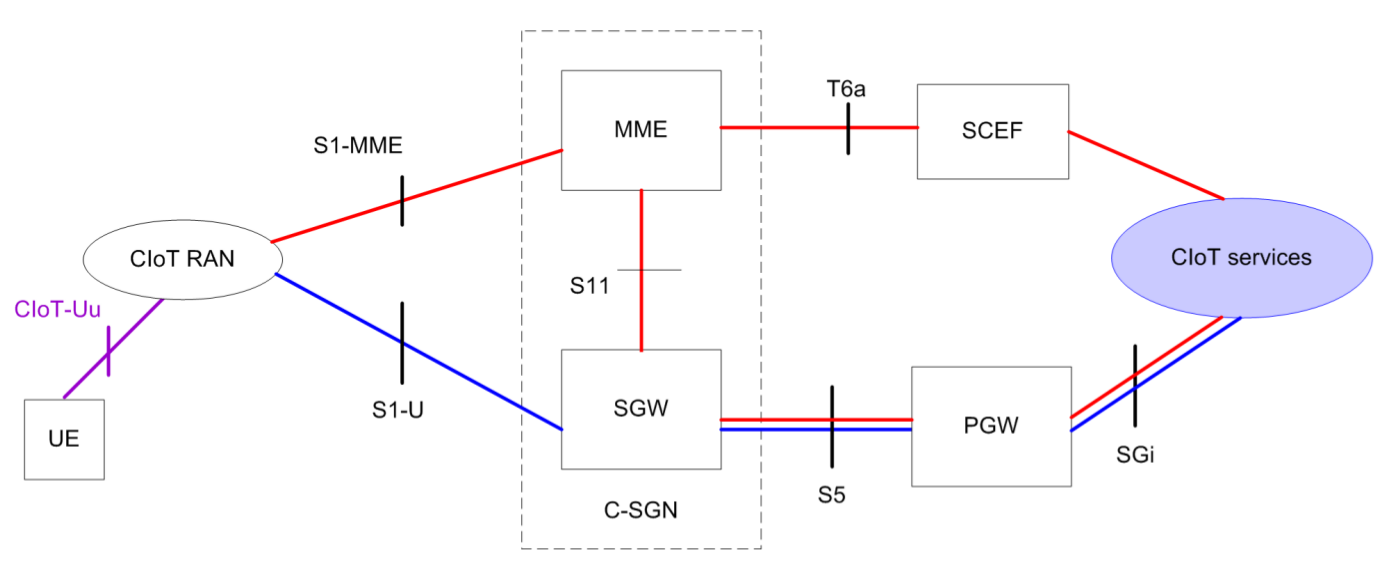
\includegraphics[width=\textwidth]{figures/NB-Network.png}
\definecolor{purple}{HTML}{7030A0}
\usetikzlibrary{arrows}
\definecolor{red}{HTML}{FF0000}
\definecolor{blue}{HTML}{00B0F0}

\resizebox{\textwidth}{!}{
\begin{tikzpicture}[scale=0.5]


\draw  (-14,5) rectangle (-10,3);
\node at (-12,4) {Device};
\draw  (-4,14) rectangle (2,-8);
\draw  (6,9) rectangle (10,7);
\draw  (6,1) rectangle (10,-1);
\node at (-1,-7) {\acrshort{CIoT} \acrshort{RAN}};
\node at (8,8) {\acrshort{MME}};
\node at (8,0) {\acrshort{SGW}};
 




\draw  (14,1) rectangle (18,-1);
\draw  (14,13) rectangle (18,11);
\draw  (25,6) ellipse (3 and 2);
\node at (16,12) {\acrshort{SCEF}};

\node at (16,0) {\acrshort{PGW}};
\node at (25,6) {\acrshort{CIoT} Services};

\draw  (-3,13) rectangle (1,11);
\draw  (-3,5) rectangle (1,3);
\draw  (-3,-3) rectangle (1,-5);
\node at (-1,12) {\acrshort{eNB}};
\node at (-1,4) {\acrshort{eNB}};
\node at (-1,-4) {\acrshort{eNB}};

\draw (6,18) -- (6,15); 
\draw (10,15) -- (10,18);
\draw  (8,18) ellipse (2 and 0.5);
\node at (8,15.4) {\acrshort{HSS}};
\draw (6,15) arc (-120:-60:4);

\draw (14,8.6) -- (14,5.6);
\draw (18,5.6) -- (18,8.6);
\draw  (16,8.6) ellipse (2 and 0.5);
\node at (16,6) {\acrshort{PCRF}};
\draw (14,5.6) arc (-120:-60:4);
\node (v27) at (16,5) {};


\node (v2) at (-7,4) {\acrshort{CIoT}-Uu};
\node (v1) at (-10,4) {};
\node (v3) at (-4,4) {};
\draw [draw=purple, arrows={triangle 45-},fill=purple] (v1) edge (v2);
\draw [draw=purple, arrows={-triangle 45},fill=purple] (v2) edge (v3);

\node (v5) at (-1,8) {X2};
\node (v8) at (-1,0) {X2};
\node (v4) at (-1,11) {};
\node (v6) at (-1,5) {};
\node (v7) at (-1,3) {};
\node (v9) at (-1,-3) {};
\draw [draw=red, arrows={triangle 45-},fill=red] (v4) edge (v5);
\draw [draw=red, arrows={-triangle 45},fill=red] (v5) edge (v6);
\draw [draw=red, arrows={triangle 45-},fill=red] (v7) edge (v8);
\draw [draw=red, arrows={-triangle 45},fill=red] (v8) edge (v9);
\node (v10) at (2,4) {};
\node (v14) at (6,0) {};
\node (v12) at (6,8) {};
\node (v18) at (8,7) {};
\node (v20) at (8,1) {};
\node (v17) at (8,9) {};
\node (v15) at (8,14.4) {};
\node (v21) at (10,8) {};
\node (v23) at (14,12) {};

\node (v24) at (10,0) {};
\node (v26) at (14,0) {};

\node (v33) at (18,0) {};
\node (v32) at (22,6) {};
\node (v30) at (18,12) {};
\node (v29) at (16,1) {};

\node (v11) at (4,6) {S1-\acrshort{MME}};
\node (v13) at (4,2) {S1-U};
\node (v19) at (8,4) {S11};
\node (v16) at (8,12) {S6a};
\node (v22) at (12,10) {T6a};
\node (v25) at (12,0) {S5};
\node (v28) at (16,3) {S7};
%\node (v31) at (20,9) {};
\node (v34) at (20,3) {SGi};

\draw [draw=red, arrows={triangle 45-},fill=red]  (v10) edge (v11);
\draw [draw=red, arrows={-triangle 45},fill=red]  (v11) edge (v12);
\draw [draw=blue, arrows={triangle 45-},fill=blue]  (v10) edge (v13);
\draw [draw=blue, arrows={-triangle 45},fill=blue]  (v13) edge (v14);


\draw [draw=red, arrows={triangle 45-},fill=red]   (v15) edge (v16);
\draw [draw=red, arrows={-triangle 45},fill=red]  (v16) edge (v17);
\draw [draw=red, arrows={triangle 45-},fill=red]  (v18) edge (v19);
\draw [draw=red, arrows={-triangle 45},fill=red]  (v19) edge (v20);
\draw [draw=red, arrows={triangle 45-},fill=red]  (v21) edge (v22);
\draw [draw=red, arrows={-triangle 45},fill=red]  (v22) edge (v23);
\draw [draw=purple, arrows={triangle 45-},fill=purple]  (v24) edge (v25);
\draw [draw=purple, arrows={-triangle 45},fill=purple]  (v25) edge (v26);
\draw [draw=red, arrows={triangle 45-},fill=red]  (v27) edge (v28);
\draw [draw=red, arrows={-triangle 45},fill=red]  (v28) edge (v29);
\draw [draw=red, arrows={triangle 45-triangle 45},fill=red]  (v30) edge (v32);
%\draw [draw=red, arrows={-triangle 45},fill=red]  (v31) edge (v32);
\draw [draw=purple, arrows={triangle 45-},fill=purple]  (v33) edge (v34);
\draw [draw=purple, arrows={-triangle 45},fill=purple]  (v34) edge (v32);
\end{tikzpicture}
}
\caption{Overview over the network blocks and interfaces between blocks in \gls{NB-IoT}. Blue lines are user plane \gls{CIoT} \gls{EPS} optimization, the red lines are control plane \gls{CIoT} \gls{EPS} optimization plane and the purple lines are both \citep{NB_slide}}
\label{fig:network_structure}
\end{figure}


\textbf{\gls{UE}}\\
The \gls{UE} is the smart meters or other products as mentioned, they do not need to transmit a lot of data and it is not critical that it arrives within a certain time frame. They do however require a long battery life time. The problem comes in terms of placement, because many of these devices might be placed in basement like environment which means an increased path loss. The system needs to be able to operate with a \gls{MCL} of 164 dB \citep{REL-13}. As in previous systems the \gls{USIM} is located on the \gls{UE} for authentication purpose \citep[ch. 3]{book_LTE_for_UMTS}.

\textbf{\gls{CIoT} \gls{RAN}}\\
The \gls{CIoT} \gls{RAN} is the base stations, the most typically used is the \gls{eNB} base station. All radio communication terminates at this node. Any \gls{UE} that wish to use an external service, interfaces with the \gls{eNB} \citep{book_LTE_for_UMTS}. The \gls{eNB} interfaces with both the \gls{MME} and the \gls{SGW}. On the control plane (connection to the \gls{MME}) the \gls{eNB} is in charge of \gls{RRM}, i.e. allocating radio resources in the user plane to the individual \gls{UE} based on \gls{QoS} measures. 

\textbf{\gls{MME}}\\
The \gls{MME} takes care of mobility issues, it also keep track of where in the network different \gls{UE}s are connected \citepalias{3GPP_MME_spec}. Another very important function of the \gls{MME} is to handle authentication of \gls{UE}s and setting up security for the data bearers. The \gls{MME} might be connected to multiple \gls{UE}s, however a \gls{UE} may only be connected to a single \gls{MME} \citep[ch. 3]{book_LTE_for_UMTS}. In \gls{NB-IoT} handovers are omitted and the only way to change cell is by releasing the existing connection \citep{REL-13}. The \gls{MME} also handles paging procedures \citep{NB-IoT_Book}.

\textbf{\gls{HSS}}\\
The \gls{HSS} stores the identity of the users, which the \gls{MME} uses for authentication purposes. It records the location of the \gls{UE} in level of visited network control nodes  such as \gls{MME}, it also keep track of which networks the user is allowed to roam to \citep[ch. 3]{book_LTE_for_UMTS}.

\textbf{\gls{SCEF}}\\
The \gls{SCEF} is a multi functional unit, task it handles include: device trigger delivery, sponsored data, \gls{UE} reachability, \gls{3GPP} network issues, \gls{QoS} for a \gls{UE} session etc. Many of these functionalities are meant for normal \gls{LTE} use. Uses meant for \gls{NB-IoT} include \gls{UE} reachability which enables the application layer to be informed when a \gls{UE} reconnects to the network i.e. after an \gls{eDRX} or after \gls{PSM}. Another functionality it handles is \gls{NIDD}, which enables \gls{UE}s with small data volumes to send it data with less overhead and thereby have a longer battery life time \citepalias{3GPP_SCEF_primer}.

\textbf{\gls{SGW}}\\
The \gls{SGW} is primarily a routing unit. It interfaces with the \gls{eNB}, the \gls{MME} and the \gls{PGW}. When the \gls{UE} transmit data it is send to the \gls{eNB} and then routed via the \gls{SGW} to the \gls{PGW} before reaching the providers. The \gls{SGW} typically serve a particular geographic area with several \gls{eNB}s, likewise could the \gls{MME} also serve a particular geographic area. In \gls{LTE} this was the last node in the network that could change during a connected state meaning that all \gls{SGW}s needs to be connected to all \gls{PGW}s \citep[ch. 3]{book_LTE_for_UMTS}. This is however not equally important in \gls{NB-IoT} as no handovers are expected \citep{REL-13}. During connected state the \gls{SGW} works as a relay, however in idle mode the resources are released in the \gls{eNB} and the data path terminates at the \gls{SGW} it then stores the data from the \gls{PGW} and request the \gls{MME} to initiate paging of the \gls{UE} \citep[ch. 3]{book_LTE_for_UMTS}.

\textbf{\gls{PGW}}\\
The \gls{PGW} is the edge of the \gls{EPS}. It function as the point of attachment for the \gls{UE}s \gls{IP} traffic. The \gls{IP}-address of the \gls{UE} is allocated during the connection procedure when the \gls{UE} request a \gls{PDN} connection and during any subsequent \gls{PDN} connection request. It is the \gls{PGW} that performs the \gls{DHCP} functionality \citep[ch. 3]{book_LTE_for_UMTS}. The \gls{PGW} handle interfaces to external CIoT services on a higher level.

\textbf{\gls{PCRF}}\\
The \gls{PCRF} is a server that makes decision on how to handle services provided for the \gls{UE} in terms of \gls{QoS}. It informs the \gls{PGW} and if applicable the \gls{SGW} about appropriate bearer policy can be set up. A default bearer is set up during connection request and either the \gls{UE} or the service domain can request additional bearers which is handled by the \gls{PCRF} \citep[ch. 3]{book_LTE_for_UMTS}.

\textbf{\gls{CIoT} services}\\
The \gls{CIoT} services are typically storage functionalities, but could be control algorithms or other services needed for specific products. 

%connections across the network

\section{Protocol Layers}

The following section is focused on the communication protocol in the \gls{CIoT}-Uu interface. It consist of the following six layers:
\begin{itemize}
	\item \gls{NAS} layer
	\item \gls{RRC} layer
	\item \gls{PDCP} layer
	\item \gls{RLC} layer
	\item \gls{MAC} layer
	\item \gls{PHY} layer
\end{itemize}

The purpose and functionalities of these layers are explained in the following.

\subsection{NAS}
The \gls{NAS} layer is the top layer in the control plane. It signals directly between the device and the \gls{MME} \citep[ch. 3]{book_LTE_for_UMTS}. There are two protocols in the \gls{NAS} layer, the \gls{EMM} and the \gls{ESM}. The \gls{EMM} handles re-activation from idle mode: the device initiated case is called service request, the network initiated case is called paging. The \gls{EMM} protocol is used for handling attachment and detachment from the system when the device is in idle mode. In connected mode lower layer protocols handles this instead \citep[ch. 3]{book_LTE_for_UMTS}. In the NB-IoT protocol, a functionality has been implemented, to transmit data directly through the NAS layer \citep{REL-13}. 

\subsection{RRC} \label{sec:RRC}
The \gls{RRC} layer of the protocol is a strictly control plane layer. The functionalities provided by the \gls{RRC} are \citep[ch. 6.6]{book_LTE_for_UMTS}:

\begin{itemize}
	\item Broadcast of system information
	\item Paging
	\item Establishment, maintenance and release of an \gls{RRC} connection between device and the \gls{eNB}
	\item Security functions, including key management
	\item Establishment, maintenance and release of point to point radio bearers
	\item Device measurement reporting and control of the reporting
	%\item Handover
	\item Device cell selection and reselections 
%	\item Context transfer between \gls{eNB}s
	\item Device capability transfer
	\item Generic protocol error handling
	\item Support of self-configuration and self-optimization
\end{itemize}

One of the biggest changes from \gls{LTE} to \gls{NB-IoT} is the focus on reducing power consumption. Therefore a new state has been introduced compared to the \gls{LTE} system, which can be seen on \autoref{fig:UE-states}.

\tikzsetnextfilename{state-diagram}
\begin{figure}[H]
\centering
\usetikzlibrary{arrows}
%\usetikzlibrary{shapes.multipart}
\renewcommand{\arraystretch}{0.8}
\resizebox{\textwidth}{!}{
\begin{tikzpicture}[scale=0.5]

\draw  (-26,28) ellipse (3 and 2);
\node at (-26,28) {Start up};

\draw  (-17,28) ellipse (3 and 2);
\node at (-17,28) {Idle state};

\draw  (-24.5,11) ellipse (3 and 2);
%\node at (-17,15) {\acrshort{PSM}};
\node at (-24.5,11) {PSM};

\draw  (-10,19.5) rectangle (-4,16.5);
\node at (-7,18) {\begin{tabular}{c} Resume RRC \\ connection \end{tabular}};

\draw  (-10,26.5) rectangle (-4,23.5);
\node at (-7,25) {\begin{tabular}{c} Establish RRC \\ connection\end{tabular}};

\draw  (-10,13.5) rectangle (-4,10.5);
\node at (-7,12) {\begin{tabular}{c} Suspend RRC \\ connection\end{tabular}};

\draw  (-10,32.5) rectangle (-4,29.5);
\node at (-7,31) {\begin{tabular}{c} Release RRC \\ connection\end{tabular}};

\draw  (4,21.5) ellipse (3 and 2);
\node at (4,21.5) {Connected state};

\draw  (-17,15) ellipse (3 and 2);
\node at (-17,15) {\begin{tabular}{c} Idle state \\ (with AS)\end{tabular}};
\node (v22) at (-20,15) {};
\node (v23) at (-14,15) {};

\draw  (-24.5,19) ellipse (3 and 2);
\node at (-24.5,19) {eDRX};
\node (v25) at (-19,16.5) {};
\node (v26) at (-22,18) {};
\node (v27) at (-22.5,17.5) {};
\node (v28) at (-19.5,16) {};
\node[rotate=27] at (-21.5,14) {\begin{tabular}{c} PSM\\ command\end{tabular}};
\node[rotate=27] at (-20.25,12.25) {Timer};




\node (v1) at (-23,28) {};
\node (v2) at (-20,28) {};
\node (v3) at (-14,28) {};
\node (v4) at (-10,25) {};
\node (v5) at (-4,25) {};
\node (v6) at (1,21.5) {};
\node (v7) at (-4,12) {};
\node (v8) at (-4,31) {};
\node (v9) at (-4,18) {};
\node (v10) at (-10,18) {};
\node (v11) at (-10,12) {};
\node (v12) at (-10,31) {};
\node (v13) at (-7,19.5) {};
\node (v14) at (-7,23.5) {};
\node (v15) at (-19.5,14) {};
\node (v16) at (-22.5,12.5) {};
\node (v17) at (-22,12) {};
\node (v18) at (-19,13.5) {};



\draw [arrows={- triangle 45}] (v1) edge (v2);
\draw [arrows={- triangle 45}] (v23) edge (v10);
\draw [arrows={- triangle 45}] (v3) edge (v4);
%\draw [arrows={triangle 45-}]  (v4) edge ($(midpoint)+(0,0)$);

\draw [arrows={- triangle 45}] (v11) edge (v23);
\draw [arrows={- triangle 45}] (v12) edge (v3);
\draw [arrows={- triangle 45}] (v13) edge (v14);
\draw [arrows={- triangle 45}] (v9) edge (v6);
\draw [arrows={- triangle 45}] (v5) edge (v6);
\draw [arrows={- triangle 45}] (v6) edge (v7);
\draw [arrows={- triangle 45}] (v6) edge (v8);
\draw [arrows={- triangle 45}] (v15) edge (v16);
\draw [arrows={- triangle 45}]  (v17) edge (v18);
\draw [arrows={- triangle 45}] (v25) edge (v26);
\draw [arrows={- triangle 45}]  (v27) edge (v28);


\node at (-21.75,28.5) {Sync};
\node[rotate=-27] at (-20,18) {\begin{tabular}{c} eDRX \\ command\end{tabular}};
\node[rotate=-27] at (-21.25,16.25) {Timer};
\node[rotate=39] at (-12.2,30) {Ok};
\node[rotate=39] at (-12.2,17.1) {Data/paging};
\node[rotate=-39] at (-12.2,13) {Ok};
\node[rotate=-39] at (-12.4,26.1) {Data};
\node[rotate=-35] at (-2,24.2) {Complete};
\node[rotate=35] at (-2,20) {Complete};
\node[rotate=62] at (-0.8,16.8) {No more data};
\node[rotate=-62] at (-0.8,26.2) {No more data};
\node[rotate=90] at (-7.5,21.5) {Reject};


\end{tikzpicture}
}
\caption{State diagram with transition options for a device.}
\label{fig:UE-states}
\end{figure}


With this new structure comes a greater focus on \gls{RRC} connection resume, which is very advantageous with regards to power consumption, as it allows the device to suspend its connection and save its \gls{AS}, when going into idle mode.

This enables the device to request a connection resume, where it uses its previous \gls{AS} to reduces the overhead considerably. This can also be seen from \autoref{tab:signaling_comparison} where a comparison between the different procedures is shown. 

\begin{table}[H]
\centering
\resizebox{\textwidth}{!}{
\begin{tabular}{|p{2.5cm}|p{4cm}|p{4cm}|p{4cm}|} \hline
\rowcolor{gray!50}\textbf{Direction} & \raggedright\arraybackslash\textbf{Legacy Service Request Procedure}	& \raggedright\arraybackslash\textbf{\gls{RRC} Connection Resume} & \textbf{Control Plane Data Transfer}  \\\hline
UL	& \multicolumn{3}{c|}{Preamble} \\\hline
\rowcolor{gray!10}DL	& \multicolumn{3}{c|}{\gls{RAR}} \\\hline
UL	& \raggedright\arraybackslash \gls{RRC} Connection Request						& \raggedright\arraybackslash \gls{RRC} Connection Resume Request	& \raggedright\arraybackslash \gls{RRC} Connection Request \\\hline
\rowcolor{gray!10}DL	& \raggedright\arraybackslash \gls{RRC} Connection Setup						& \raggedright\arraybackslash \gls{RRC} Connection Resume 			& \raggedright\arraybackslash \gls{RRC} Connection Setup   \\\hline
UL	& \raggedright\arraybackslash \gls{RRC} Connection Request Complete 			& \raggedright\arraybackslash \gls{RRC} Connection Resume Complete & \raggedright\arraybackslash \gls{RRC} Connection Complete  \\\hline
\rowcolor{gray!10}DL	& \raggedright\arraybackslash Security Mode Command 							& - & -  \\\hline
UL	& \raggedright\arraybackslash Security Mode Complete 							& - & -  \\\hline
\rowcolor{gray!10}DL	& \raggedright\arraybackslash \gls{RRC} Connection Reconfiguration 			& - & -  \\\hline
UL	& \raggedright\arraybackslash \gls{RRC} Connection Reconfiguration Complete 	& - & -  \\\hline
\raggedright\arraybackslash \textbf{Total number of messages} 					& \textbf{9} & \textbf{5} & \textbf{5} \\\hline
\end{tabular}
}
\caption{Signaling comparison between different methods \citep{REL-13}.}
\label{tab:signaling_comparison}
\end{table}

\textbf{\Gls{SRB}}\\
The \gls{RRC} sets up three different \gls{SRB}s, which are used to carry \gls{RRC} and \gls{NAS} messages. \gls{SRB}0 is used for \gls{CCCH} during \gls{RRC} connection setup or during link failure. Messages carried here include \gls{RRC} connection request, \gls{RRC} connection setup, \gls{RRC} connection reject, \gls{RRC} connection reestablishment request, \gls{RRC} connection reestablishment and \gls{RRC} connection reestablishment reject. \gls{SRB}1 is used when a \gls{RRC} connection is established. It is used to transfer both \gls{RRC} messages, using \gls{DCCH}, and \gls{NAS} messages until security is established. Once security is established, the \gls{NAS} messages is carried on \gls{SRB}2, which has a lower priority. \citep[ch. 6.6]{book_LTE_for_UMTS} 


\textbf{\gls{SIB}s}\\
Before the device attempts to access the system, it needs a lot of information about the system, which is carried in the \gls{SIB}s. For \gls{NB-IoT} there are eight different \gls{SIB}s messages. A list of the information carried in the different \gls{SIB}s can be seen in \autoref{tab:NB-SIB}. The \gls{RRC} takes care of updating these messages and paging the devices if changes occurs.

\begin{table}[H]
\centering
\begin{tabular}{|p{3cm}|p{8cm}|p{3cm}|}\hline
\textbf{Name}		& \textbf{Information}																	& \textbf{Update rate}	\\\hline
\raggedright\arraybackslash\gls{MIB-NB}		& Essential information required to receive further system information 					& 640 ms				\\\hline
\raggedright\arraybackslash\gls{NB-SIB}1		& Cell access and selection and the other SIBs scheduling 										& 40.96 s 				\\\hline
\gls{NB-SIB}2		& Radio resource configuration information 												& NA 					\\\hline
\gls{NB-SIB}3		& Cell re-selection information for intra-frequency, inter-frequency 					& NA 					\\\hline
\gls{NB-SIB}4		& Neighboring cell related information relevant for intra-frequency cell re-selection 	& NA 					\\\hline
\gls{NB-SIB}5		& Neighboring cell related information relevant for inter-frequency cell re-selection 	& NA 					\\\hline
\gls{NB-SIB}14		& Access barring parameters 															& Fast 					\\\hline
\gls{NB-SIB}16		& Information related to GPS time and Coordinated Universal Time (UTC) 					& Fast 					\\\hline
\end{tabular}
\caption{List of different \gls{SIB} messages and the information carried within \citep{whitepaper,REL-13}.}
\label{tab:NB-SIB}
\end{table}

\textbf{Paging} \\
Paging serves two main functions: the first is to notify a device in \gls{RRC} idle state to set up a \gls{RRC} connection to handle incoming data and the second is to inform the devices, both in \gls{RRC} idle and \gls{RRC} connected state, that the system information has changed. \citep[ch. 7]{NB-IoT_Book}

\textbf{Establishment, Maintenance and Release of \gls{RRC} Connection} \\
When an \gls{RRC} connection setup is requested, the \gls{eNB} has the option to reject it with a wait timer, if the network is overloaded. The \gls{RRC} can set the access barring parameter appropriately depending on the traffic load. In the \gls{RRC} connection request message, the device can trasmit its \gls{S-TMSI} if it possess a valid version, else it will transmit a 40 bit random value. Five different establishment causes has been defined: emergency, high-priority access, mobility-terminated access, mobile-originated signaling and mobile-originated data. In \gls{NB-SIB}1 there exists at most six different \gls{PLMN} identities, where the device selects one and reports it in the  \gls{RRC} connection setup complete message, along with any \gls{MME} the device might already be registered to. The \gls{eNB} then finds the \gls{MME} and starts the S1 connection setup. When a connection setup is successful the device moves to the \gls{RRC} connected state. \citep[ch. 6.6]{book_LTE_for_UMTS}

%\todo{should we put detailed connection options in here, should we go in detail with further RRC functions and what about radio bearers}

%\textbf{\gls{UE} Measurement Reporting and Control of the Reporting} \\


%%% pic for rrc connection resume
%\begin{figure}[H]
%\centering
%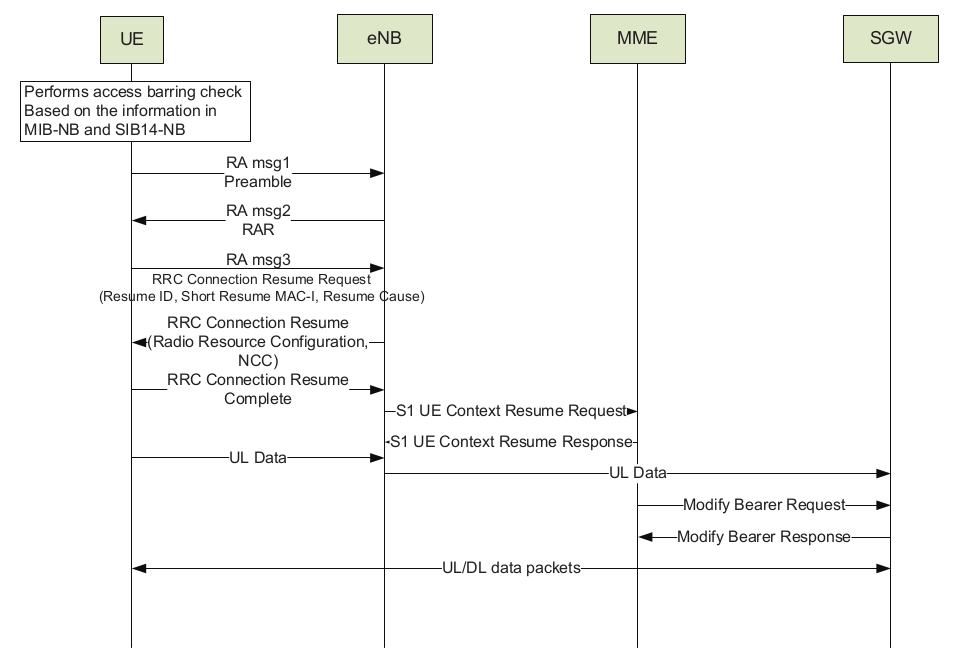
\includegraphics[width=\textwidth]{figures/RRC_resume.png}
%\caption{Signaling procedure for a \gls{RRC} resume request}
%\label{fig:RRC_resume}
%\end{figure}

\subsection{PDCP}
The \gls{PDCP} layer is just below the \gls{RRC}, where it handles both control functions as well as device data. The key function of the \gls{PDCP} include \citep[ch. 6.5]{book_LTE_for_UMTS}:
\begin{itemize}
	\item Header compression and decompression of \gls{IP} packets. This is an important function especially for small data packets, as the overhead could become quite significant
	\item Ciphering and deciphering of both user plane and most of control plane data
	\item Integrity protection and verification to ensure control data comes from the correct source
\end{itemize}

The \gls{PDCP} gets \gls{PDCP} \gls{SDU}s from the \gls{RRC} and \gls{NAS} layer. 

\tikzsetnextfilename{PDCP_data_flow}
\begin{figure}[H]
\centering
\resizebox{0.8\textwidth}{!}{
\begin{tikzpicture}[scale=.5]


\node (v2) at (-0.5,8) {NAS};
\draw  (-1,7) rectangle (-14,-9);
\draw  (0,7) rectangle (13,-9);
\node[anchor=west] at (-14,6) {Transmitting side};
\node[anchor=east] at (13,6) {Receiving side};

\draw  (-10,5) rectangle (-5,3);
\node at (-7.5,4) {\begin{tabular}{c} Sequence \\[-0.9em] numbering \end{tabular}};
\draw  (-13,1) rectangle (-8,-1);
\node at (-10.5,0) {\begin{tabular}{c} Integrity \\[-0.9em] protection \end{tabular}};
\draw  (-7,1) rectangle (-2,-1);
\node at (-4.5,0) {\begin{tabular}{c} Header \\[-0.9em] compression \end{tabular}};
\draw  (-11,-3) rectangle (-4,-5);
\node at (-7.5,-4) {Ciphering};
\draw  (-13,-6) rectangle (-7,-8) node (v1) {};
\draw  (v1) rectangle (-2,-6);
\node at (-10,-7) {PDCP header};
\node at (-4.5,-7) {Data field};
\node (v12) at (-7,-10) {RLC};

\node (v3) at (-7.5,5) {};
\node (v4) at (-7.5,3) {};
\node (v5) at (-10.5,1) {};
\node (v6) at (-4.5,1) {};
\node (v9) at (-4.5,-1) {};
\node (v7) at (-10.5,-1) {};
\node (v8) at (-7.5,-3) {};
\node (v10) at (-7,-5) {};
\node (v11) at (-4.5,-6) {};
\draw  [- triangle 45] (v2) -- (-7.5,5);
\draw  [- triangle 45] (-7.5,3) -- (-10.5,1);
\draw  [- triangle 45] (-7.5,3) -- (-4.5,1);
\draw  [- triangle 45] (-10.5,-1) -- (-7.5,-3);
\draw  [- triangle 45] (-4.5,-1) -- (-7.5,-3);
\draw  [- triangle 45] (-7.5,-5) -- (-4.5,-6);
\draw  [- triangle 45] (-7,-8) -- (v12);
\node[anchor=east] at (-9.2,2) {\begin{tabular}{c} \textbf{Control} \\[-0.9em] \textbf{Plane} \end{tabular}};
\node[anchor=west] at (-5.4,2) {\begin{tabular}{c} \textbf{User} \\[-0.9em] \textbf{Plane} \end{tabular}};

\draw  (12,5) rectangle (7,3);
\node at (9.5,4) {Reordeing};
\draw  (6,1) rectangle (1,-1);
\node at (3.5,0) {\begin{tabular}{c} Integrity \\[-0.9em] protection \end{tabular}};
\draw  (12,1) rectangle (7,-1);
\node at (9.5,0) {\begin{tabular}{c} Header \\[-0.9em] decompression \end{tabular}};
\draw  (10,-3) rectangle (3,-5);
\node at (6.5,-4) {Deciphering};
\draw  (12,-6) rectangle (7,-8) node (v1) {};
\draw  (v1) rectangle (1,-6);
\node at (4,-7) {PDCP header};
\node at (9.5,-7) {Data field};

\node (v3) at (-7.5,5) {};
\node (v4) at (-7.5,3) {};
\node (v5) at (3.5,1) {};
\node (v6) at (9.5,1) {};
\node (v9) at (9.5,-1) {};
\node (v7) at (3.5,-1) {};
\node (v8) at (6.5,-3) {};
\node (v10) at (6,-5) {};
\node (v11) at (9.5,-6) {};
\node (v14) at (9.5,3) {};
\node (v15) at (7,4) {};
\node (v13) at (7,-10) {RLC};

\draw [- triangle 45] (v13) -- (7,-8);
\draw [- triangle 45] (9.5,-6) -- (6.5,-5);
\draw [- triangle 45] (6.5,-3) -- (3.5,-1);
\draw [- triangle 45] (6.5,-3) -- (9.5,-1);
\draw [- triangle 45] (9.5,1) -- (9.5,3);
\draw [- triangle 45] (7,4) -- (v2);
\draw [arrows={triangle 45 - triangle 45}] (3.5,1) -- (v2);
\node[anchor=east] at (4.3,-2) {\begin{tabular}{c} \textbf{Control} \\[-0.9em] \textbf{Plane} \end{tabular}};
\node[anchor=west] at (8.5,-2) {\begin{tabular}{c} \textbf{User} \\[-0.9em] \textbf{Plane} \end{tabular}};

\end{tikzpicture}}
\caption{\gls{PDCP} layer operation with associated \gls{PDCP} \gls{SDU} \citep[fig. 6.12]{book_LTE_for_UMTS}.}
\label{fig:PDCP_operation}
\end{figure}

As can be seen on \autoref{fig:PDCP_operation}, before forwarding the data to the \gls{RLC} layer, it is first numbered and then either integrity protection or header compression is applied, depending on whether or not it is control plane data or user plane data. It is then ciphered and forwarded. When the \gls{PDCP} receive data from the \gls{RLC} layer, it is first deciphered and again depending on whether it is control or user plane data, is it integrity protected or header decompressed and reordered, before forwarding it to the \gls{NAS}. \citep[ch. 6.5]{book_LTE_for_UMTS}  

%The \gls{PDCP} layer also handles alot during handovers, however as handovers is out of the scope for \gls{NB-IoT} these functionalities are obsolete. 

\subsection{RLC}

The \gls{RLC} layer has three basic functionalities \cite[ch. 6.4]{book_LTE_for_UMTS}:

\begin{itemize}
	\item To transfer \gls{PDU}s from higher layers i.e. \gls{RRC}, \gls{NAS} or \gls{PDCP}
	\item Depending on the \gls{RLC} mode used, error correction with \gls{ARQ}, concatenation/segmentation, in-sequence delivery and duplicate detection may occur
	\item Protocol error handling to detect and recover from protocol error states caused by e.g. signaling errors
\end{itemize}

\captionsetup{belowskip=0em}
\begin{minipage}[H]{0.48\textwidth}
\tikzsetnextfilename{RLC_UM-SAP}
\begin{figure}[H]
\centering
\resizebox{\textwidth}{!}{
\begin{tikzpicture}[scale=.5]

\draw  (-1,8.5) rectangle (-14,-8);
\draw  (0,8.5) rectangle (13,-8);

\node (v1) at (-6,6) {Transmission Buffer};
\draw  (v1) ellipse (4 and 1);
\draw (-10,5.5) arc (180:360:4 and 1);
\draw (-10,5) arc (180:360:4 and 1);
\draw (-10,2) arc (180:360:4 and 1);
\node (v2) at (-10,6) {};
\node (v4) at (-2,6) {};
\node (v3) at (-10,1.7) {};
\node (v5) at (-2,1.7) {};
\draw  (v2) ++(0,0) edge (v3);
\draw  (v4)  ++(0,0) edge (v5);

\draw  (-9,-1) rectangle (-3,-3);
\node at (-6,-2) {\begin{tabular}{c} Segmentation/ \\[-0.9em] Concatenation\end{tabular}};
\draw  (-13,-5) rectangle (-8,-7) node (v6) {};
\draw  (v6) rectangle (-3,-5);
\node at (-10.5,-6) {UM Header};
\node at (-5.5,-6) {Data Field};



\node (v10) at (7,2) {Receiving Buffer};
\draw  (v10) ellipse (4 and 1);
\draw (3,1.5) arc (180:360:4 and 1);
\draw (3,1) arc (180:360:4 and 1);
\draw (3,-2) arc (180:360:4 and 1);
\node (v20) at (3,2) {};
\node (v40) at (11,2) {};
\node (v30) at (3,-2.3) {};
\node (v50) at (11,-2.3) {};
\draw  (v20) ++(0,0) edge (v30);
\draw  (v40)  ++(0,0) edge (v50);


\draw  (4.5,7) rectangle (9.5,5);
\draw  (1,-5) rectangle (6,-7) node (v7) {};
\draw  (v7) rectangle (11,-5);
\node at (7,6) {Reasembly};
\node at (7,-1.5) {\& HARQ Reordering};
\node at (3.5,-6) {UM Header};
\node at (8.5,-6) {Data Field};

\node (v15) at (-8,-9) {Logic Channels};
\node (v16) at (6,-9) {Logic Channels};
\node (v14) at (-5.5,-5) {};
\node (v13) at (-6,-3) {};
\node (v11) at (-6,1) {};
\node (v9) at (-6,7) {};
\node (v8) at (-1,9.5) {UM-Service Access Point};
\node (v22) at (7,7) {};
\node (v21) at (7,5) {};
\node (v19) at (7,3) {};
\node (v18) at (7,-3) {};
\node (v17) at (8.5,-5) {};
\node (v12) at (-6,-1) {};

\draw [arrows={ - triangle 45}] (v8) edge (v9);
\draw [arrows={ - triangle 45}] (v11) edge (v12);
\draw [arrows={ - triangle 45}] (v13) edge (v14);
\draw [arrows={ - triangle 45}] (v6) edge (v15);
\draw [arrows={ - triangle 45}] (v16) edge (v7);
\draw [arrows={ - triangle 45}] (v17) edge (v18);
\draw [arrows={ - triangle 45}] (v19) edge (v21);
\draw [arrows={ - triangle 45}] (v22) edge (v8);
\node [anchor=west] at (-14,7.75) {Transmitting Side};
\node [anchor=east] at (13,7.75) {Receiving Side};
\end{tikzpicture}}
\caption{\gls{RLC} \gls{UM} operation \citep[ch. 6.4]{book_LTE_for_UMTS}.}
\label{fig:RLC_AM/UM_operation2}
\end{figure}
\end{minipage}
\begin{minipage}[H]{0.48\textwidth}
\begin{figure}[H]
\tikzsetnextfilename{RLC_AM-SAP}
\centering
\resizebox{\textwidth}{!}{
\begin{tikzpicture}[scale=.5]

\draw  (-1,9) rectangle (-17,-8);
\draw  (0,9) rectangle (13,-8);

\node (v1) at (-12,6) {Transmission Buffer};
\draw  (v1) ellipse (4 and 1);
\draw (-16,5.5) arc (180:360:4 and 1);
\draw (-16,5) arc (180:360:4 and 1);
\draw (-16,2) arc (180:360:4 and 1);
\node (v2) at (-16,6) {};
\node (v4) at (-8,6) {};
\node (v3) at (-16,1.7) {};
\node (v5) at (-8,1.7) {};
\draw  (v2) ++(0,0) edge (v3);
\draw  (v4)  ++(0,0) edge (v5);

\draw  (-9,-1) rectangle (-3,-3);
\node at (-6,-2) {\begin{tabular}{c} Segmentation/ \\[-0.9em] Concatenation\end{tabular}};
\draw  (-15,-5) rectangle (-10,-7) node (v6) {};
\draw  (v6) rectangle (-5,-5);
\node at (-12.5,-6) {AM Header};
\node at (-7.5,-6) {Data Field};



\node (v10) at (7,2) {Receiving Buffer};
\draw  (v10) ellipse (4 and 1);
\draw (3,1.5) arc (180:360:4 and 1);
\draw (3,1) arc (180:360:4 and 1);
\draw (3,-2) node (v23) {} arc (180:360:4 and 1);
\node (v20) at (3,2) {};
\node (v40) at (11,2) {};
\node (v30) at (3,-2.3) {};
\node (v50) at (11,-2.3) {};
\draw  (v20) ++(0,0) edge (v30);
\draw  (v40)  ++(0,0) edge (v50);


\draw  (4.5,7) rectangle (9.5,5);
\draw  (1,-5) rectangle (6,-7) node (v7) {};
\draw  (v7) rectangle (11,-5);
\node at (7,6) {Reasembly};
\node at (7,-1.5) {};
\node at (3.5,-6) {AM Header};
\node at (8.5,-6) {Data Field};

\node (v15) at (-10,-9) {Logic Channels};
\node (v16) at (6,-9) {Logic Channels};
\node (v14) at (-7.5,-5) {};
\node (v13) at (-6,-3) {};
\node (v11) at (-12,1) {};
\node (v9) at (-12,7) {};
\node (v8) at (-0.5,10) {AM-Service Access Point};
\node (v22) at (7,7) {};
\node (v21) at (7,5) {};
\node (v19) at (7,3) {};
\node (v18) at (7,-3) {};
\node (v17) at (8.5,-5) {};
\node (v12) at (-6,-1) {};

\draw [arrows={ - triangle 45}] (v8) -- (-12,7);
\draw [arrows={ - triangle 45}] (-12,1) -- (-6,-1);
\draw [arrows={ - triangle 45}] (-6,-3) -- (-7.5,-5);
\draw [arrows={ - triangle 45}] (-10,-7) -- (v15);
\draw [arrows={ - triangle 45}] (v16) -- (6,-7);
\draw [arrows={ - triangle 45}] (8.5,-5) -- (7,-3);
\draw [arrows={ - triangle 45}] (7,3) -- (7,5);
\draw [arrows={ - triangle 45}] (7,7) -- (v8);
\node [anchor=west] at (-17,8) {Transmitting side};
\node [anchor=east] at (13,8) {Receiving side};
\draw  (-10,-1) rectangle (-16,-3);
\node at (-13,-2) {\begin{tabular}{c} Retransmission \\[-0.9em] Buffer\end{tabular}};
\draw  (-7,4) rectangle (-2,2) node (v24) {};
\node at (-4.5,3) {Control};
\draw [arrows={ - triangle 45}] (3,-2) -- (-2,2);
\node [anchor=west] at (0,1) {Status};
\node (v25) at (-10.2,-2) {};
\node (v26) at (-8.8,-2) {};
\node (v27) at (-13.5,-3) {};
\draw [arrows={ - triangle 45}] (-10,-2) -- (-9,-2);
\draw [arrows={ - triangle 45}] (-13.5,-3) -- (-7.5,-5);
\end{tikzpicture}}
\caption{\gls{RLC} \gls{AM} operation \citep[ch. 6.4]{book_LTE_for_UMTS}.}
\label{fig:RLC_AM/UM_operation}
\end{figure}
\end{minipage}
\captionsetup{belowskip=-1.5em}


The modes mentioned before include \gls{TM}, \gls{UM} and \gls{AM} \citep[ch. 6.4]{book_LTE_for_UMTS}, with the differences shown on \autoref{fig:RLC_AM/UM_operation} and \autoref{fig:RLC_AM/UM_operation2}, with the exception of TM.

\textbf{\gls{TM} operation} \\
In \gls{TM}, the \gls{RLC} receives and deliver the \gls{PDU}s without adding any header to it. Therefore it does not track received \gls{PDU}s between receiving and transmitting entities. This mode is only suitable for communication that does not require physical layer retransmission or the data is not sensitive to delivery order.

\textbf{\gls{UM} operation} \\
The \gls{UM} adds some control functions to the data stream. It enables segmentation of the data and keeps track of sequence numbering. This mode also makes in-sequence delivery of out-of-sequence data, which can occur because of lower layer \gls{HARQ} operation. The data is segmented and a header is added which includes a sequence number to facilitate reordering and duplicate detection on the receiving side.

\textbf{\gls{AM} operation} \\
The \gls{AM} adds all the functionalities of the \gls{UM} but also provide retransmission. The header will in this case contain information about the last correctly received packet on the receiving side additionally to the sequence number. 

In \gls{LTE} several logic channels are defined in the \gls{RLC} layer, three for uplink and five for downlink \citep[ch. 6.3]{book_LTE_for_UMTS}. 

Common logical channels:
\begin{itemize}
\item The \gls{CCCH} is used to transport control information before a \gls{RRC} connection established
\item The \gls{DCCH} is used to transport control information after a \gls{RRC} connection is established
\item The \gls{DTCH} is used to carry application data
\end{itemize}
Downlink specific logical channels:
\begin{itemize}
\item The \gls{BCCH} is used to carry the system information and other system access related information
\item The \gls{PCCH} is used to carry paging information to reach devices that are not in connected mode
%\item The \gls{MCCH}
%\item \gls{MTCH}
\end{itemize}
%\todo{missing something about the logical channels CCCH DCCH DTCH PCCH BCCH MCCH MTCH}

\subsection{MAC}

The \gls{MAC} layer takes care of several things. It maps the logical channels from the RLC layer to the transport channels. Five transport channels are defined: the \gls{RACH}, the \gls{UL-SCH}, the \gls{DL-SCH}, the \gls{BCH} and the \gls{PCH}. All logical channels are mapped to these depending on the direction of the information as can be seen on \autoref{fig:MAC_PDU_DL} and \autoref{fig:MAC_PDU_UL}. The \gls{RACH} handles the \gls{RAP}, which is solely a \gls{MAC} layer functionality with no logic channel mapped to it. The \gls{MAC} layer further handles multiplexing/demultiplexing of \gls{RLC} \gls{PDU}s into \gls{TB}s for the physical layer, including padding if a \gls{PDU} is not completely filled with data. It also handles traffic volume measurement and reports this information to the \gls{RRC} layer. Another function the \gls{MAC} layer handles is the error correction through \gls{HARQ}, along with scheduling of the physical layer. The final thing the \gls{MAC} layer handles is the transport format selection, which includes \gls{AL}, \gls{MCS} and power ramping.  

\captionsetup{belowskip=0em}
\begin{minipage}{0.48\textwidth}
	\tikzsetnextfilename{MAC_DL-mapping}
	\begin{figure}[H]
	\centering
	\resizebox{\textwidth}{!}{
	\begin{tikzpicture}[scale=.5]

\node at (-10,5) {RLC};
\node at (-10,1) {MAC};
\node at (-10,-3) {L1};

\node (v1) at (-6,5) {BCCH};
\node (v2) at (-6,1) {BCH};
\node (v3) at (-6,-3) {PBCH};

\node (v5) at (-2,5) {PCCH};
\node (v6) at (-2,1) {PCH};

\node (v8) at (2,5) {CCCH};

\node (v9) at (6,5) {DCCH};

\node (v10) at (10,5) {DTCH};
\node (v4) at (4,1) {DL-SCH};
\node (v7) at (4,-3) {PDSCH};

%\node (v11) at (14,5) {MCCH};
%
%\node (v12) at (18,5) {MTCH};
%\node (v13) at (18,1) {MCH};
%\node (v14) at (18,-3) {PMCH};

\draw [arrows={-triangle 45}] (v1) edge (v2);
\draw [arrows={-triangle 45}] (v2) edge (v3);
\draw [arrows={-triangle 45}] (v1) edge (v4);
\draw [arrows={-triangle 45}] (v5) edge (v6);
\draw [arrows={-triangle 45}] (v6) edge (v7);
\draw [arrows={-triangle 45}] (v8) edge (v4);
\draw [arrows={-triangle 45}] (v9) edge (v4);
\draw [arrows={-triangle 45}] (v10) edge (v4);
\draw [arrows={-triangle 45}] (v4) edge (v7);
%\draw [arrows={-triangle 45}] (v11) edge (v4);
%\draw [arrows={-triangle 45}] (v12) edge (v4);
%\draw [arrows={-triangle 45}] (v12) edge (v13);
%\draw [arrows={-triangle 45}] (v13) edge (v14);
\end{tikzpicture}}
	\caption{\gls{MAC} layer \gls{DL} mapping structure \citep[Sec. 6.3]{book_LTE_for_UMTS}.}
	\label{fig:MAC_PDU_DL}
	\end{figure}
\end{minipage}
\begin{minipage}{0.48\textwidth}
	\tikzsetnextfilename{MAC_UL-mapping}
	\begin{figure}[H]
	\centering
	\resizebox{\textwidth}{!}{
	\begin{tikzpicture}[scale=.5]

\node at (-10,5) {Logical chnnels};
\node at (-10,1) {Transport channels};
\node at (-10,-3) {Physical channels};

\node (v1) at (-4,1) {RACH};
\node (v2) at (-4,-3) {PRACH};

\node (v3) at (0,5) {CCCH};

\node (v4) at (4,5) {DCCH};

\node (v5) at (8,5) {DTCH};
\node (v6) at (4,1) {UL-SCH};
\node (v7) at (4,-3) {PUSCH};


\draw [arrows={-triangle 45}] (v1) edge (v2);
\draw [arrows={-triangle 45}] (v3) edge (v6);
 \draw [arrows={-triangle 45}] (v4) edge (v6);
 \draw [arrows={-triangle 45}] (v5) edge (v6);
 \draw [arrows={-triangle 45}] (v6) edge (v7);
\end{tikzpicture}}
	\caption{\gls{MAC} layer \gls{UL} mapping structure \citep[Sec. 6.3]{book_LTE_for_UMTS}.}
	\label{fig:MAC_PDU_UL}
	\end{figure}
\end{minipage}
\captionsetup{belowskip=-1.5em}

A \gls{MAC} \gls{PDU} consist of the \gls{MAC} header, the \gls{MAC} control elements, the \gls{MAC} \gls{SDU}s and potentially some padding as can be seen in \autoref{fig:MAC_PDU}

\tikzsetnextfilename{MAC_PDU}
\begin{figure}[H]
\centering
\resizebox{\textwidth}{!}{
\usetikzlibrary{decorations.pathreplacing}
\begin{tikzpicture}[scale=.5]

\draw  (-10,8) rectangle (5,-6);
\node [anchor=west] at (-9,7) {DL-SCH Types of payload elements};
\node [anchor=west] at (-9,5) {• Logical channel identity};
\node [anchor=west] at (-9,3) {• CCCH};
\node [anchor=west] at (-9,1) {• UE contention resolution identity};
\node [anchor=west] at (-9,-1) {• Timing advance};
\node [anchor=west] at (-9,-3) {• DRX command};
\node [anchor=west] at (-9,-5) {• Field length};

\draw  (6,8) rectangle (21,-6) {};
\node [anchor=west] at (7,7) {UL-SCH Types of payload elements};
\node [anchor=west] at (7,5) {• Logical channel identity};
\node [anchor=west] at (7,3) {• CCCH};
\node [anchor=west] at (7,1) {• Power headroom report};
\node [anchor=west] at (7,-1) {• C-RNTI};
\node [anchor=west] at (7,-3) {• Short buffer status report};
\node [anchor=west] at (7,-5) {• Long buffer status report};

\draw  (22,2) rectangle (37,-6) node (v4) {};
\node [anchor=west] at (23,1) {RACH Types of payload elements};
\node [anchor=west] at (23,-1) {• Type};
\node [anchor=west] at (23,-3) {• Back-off indicator};
\node [anchor=west] at (23,-5) {• Random access preamble identifier};

\draw  (-8,-9) node (v2) {} rectangle (1,-11);
\node at (-3.5,-10) {MAC Header};
\draw  (1,-9) node (v3) {} rectangle (10,-11);
\node at (5.5,-10) {MAC Control Elements};
\draw  (10,-9) rectangle (16,-11);
\node at (13,-10) {MAC SDU};
\node at (17.5,-10) {...};
\draw  (19,-9) rectangle (25,-11);
\node at (22,-10) {MAC SDU};
\draw  (25,-9) rectangle (31,-11);
\node at (28,-10) {Padding};

\node (v1) at (-10,-6) {};
\draw [dashed] (-10,-6) -- (-8,-9);
\draw [dashed] (1,-9) -- (37,-6);
\node (v5) at (1,-11.5) {};
\node (v6) at (31,-11.5) {};
\draw [decorate,decoration={brace,amplitude=15pt}] (v6) -- (v5);
\node [anchor=north] at (15.5,-13) {Payload with type indicated in header};
\end{tikzpicture}}
\caption{MAC PDU structure \citep[Sec. 6.3]{book_LTE_for_UMTS}.}
\label{fig:MAC_PDU}
\end{figure}

The header is different depending upon which transport channel is used, as can be seen on \autoref{fig:MAC_PDU}. It include key parameters for control of both the physical layer as well as the logical channel identity. It is also the \gls{MAC} layer that handles contention resolution with \gls{HARQ}, which requires the header to include \gls{CCCH} and \gls{C-RNTI} for the device. When a device tries to connect to the network, the \gls{MAC} layer also calculates timing advance. \citep[Sec. 6.3]{book_LTE_for_UMTS}


\subsection{PHY}\label{sec:NB-IoT/Physical Layer}

To accommodate the new requirements set by the \gls{IoT} development, as described in the beginning of \autoref{ch:NB-IoT}, the physical layer design also needs to be revised. The idea is to allow for three different deployments methods: in-band, guard-band and standalone \citep{primer}. This is to take advantage of the existing \gls{LTE} and \gls{GSM} networks. The idea behind the three deployments can be seen on \autoref{fig:NB deployment}. The in-band mode takes up one of the \gls{PRB} from the \gls{LTE} cell, where the guard-band mode places it just outside the LTE carriers. This is possible because none of the \gls{LTE} cells utilize the entire allocated spectrum to reduce the spectral disturbance. The proposed design also allows for the standalone case to utilize a \gls{GSM} band taking advantage of the lower frequency compared to legacy \gls{LTE} to increase the coverage area. To work inside and alongside these system provides some restrictions that needs to be respected. Therefore is the physical structure of the system the same for all deployment methods, however the use and spectrum allocation differs slightly. The most commonly discussed deployment scenario is the in-band operation as this set the most restriction for the \gls{NB-IoT} system. \citep{REL-13,primer}

\begin{figure}[H]
\centering
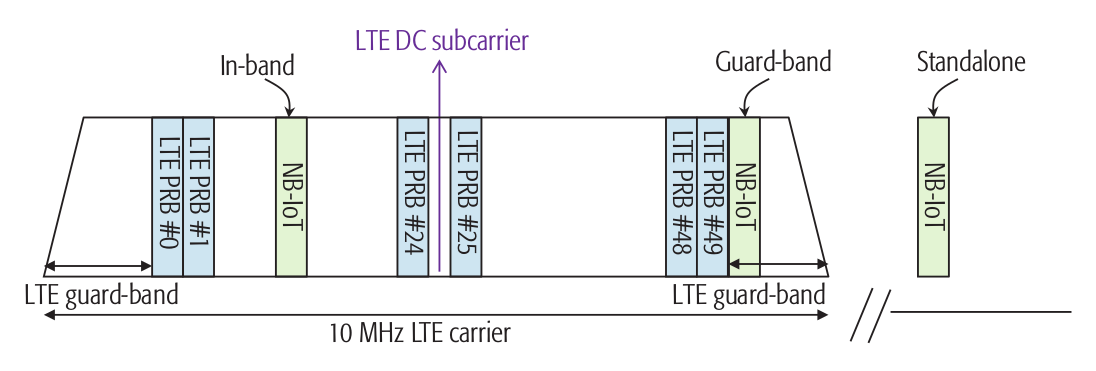
\includegraphics[width=\textwidth]{figures/deployment.png}
\caption{Deployment of the NB-IoT as in-band, guard-band or standalone \citep{primer}.}
\label{fig:NB deployment}
\end{figure}

To allow in-band operation, the physical layer of \gls{NB-IoT} needs to follow the overall structure of \gls{LTE}. To describe this, it is split into the \gls{DL} and \gls{UL} part. First the \gls{DL} part will be investigated as this accounts for most of the critical factors of the communication i.e. synchronization and system information. 

\subsubsection{Downlink}
As the primary users of legacy \gls{LTE} does not know of the \gls{NB-IoT} system, the primary concern is the interference it causes. Some structural guidelines is therefore needed when designing the \gls{NB-IoT} system, here under it needs to blend in with the \gls{OFDM} symbols of the \gls{LTE} system, meaning that timing alignment and subcarrier spacing is already determined \citep[ch. 7.2]{NB-IoT_Book}. 

Channel Raster\\
As \gls{NB-IoT} functions as an individual system, it needs it own overhead. To ensure the functionality of both systems, the \gls{PRB}s used for \gls{NB-IoT} is therefore placed outside the six center \gls{PRB}'s, as these are used for LTE synchronization. This implies that only the LTE cells with a bandwidth larger than 1.4 MHz can host NB-IoT \citep{whitepaper}. Furthermore to keep the receiver complexity and the battery consumption at a minimum, the device searches for the \gls{NB-IoT} cell on a raster of 100 kHz \citep[ch. 7.2]{NB-IoT_Book}. The center of the bandwidth host a DC-subcarrier and the \gls{PRB}'s is placed around this. This means that the center of a PRB will be offset from the raster, for instance PRB \#25 in \autoref{fig:NB deployment} has a center of 97.5 kHz, which is 2.5 kHz off from the raster. Because of this, an additional requirement is made that only those \gls{PRB}'s, where the offset is less than 7.5 kHz can be used to host a NB-IoT cell \citep{primer}. The PRB's that fulfill this criteria can be seen in \autoref{tab:available-PRBs}. 

\begin{table}[H]
\centering
\begin{tabular}{|c|p{1.8cm}|p{1.8cm}|p{1.8cm}|p{1.8cm}|p{1.8cm}|}\hline
\textbf{LTE cell bandwidth}	& 3 MHz				& 5 MHz	& 10 MHz	& 15 MHz	& 20 MHz \\\hline
Available PRB indexes		& 2, 12	& 2, 7, 17, 22	& 4, 9, 14, 19, 30, 35, 40, 45 & 2, 7, 12, 17, 22, 27, 32, 42, 47, 52, 57, 62, 67, 72 & 4, 9, 14, 19, 24, 29, 34, 39, 44, 55, 60, 65, 70, 75, 80, 85, 90, 95 \\\hline
\end{tabular}
\caption{Available PRBs depending on the bandwidth of the LTE cell \citep{whitepaper}.}
\label{tab:available-PRBs}
\end{table}


Frame Structure\\
To fit into a \gls{LTE} \gls{PRB}, the frame structure needs to be very similar to legacy \gls{LTE}. The structure is divided into: hyperframe, frame, subframe and slots. Where two slots make a subframe, ten subframes make a frame and 1024 frames make a hyperframe. A complete cycle takes 1024 hyperframes, which corresponds to 2 hours 54 minutes and 46 seconds. This structure is shown on \autoref{fig:downlink-structure}. \citep[ch. 7.2]{NB-IoT_Book}


\begin{figure}[H]
\centering
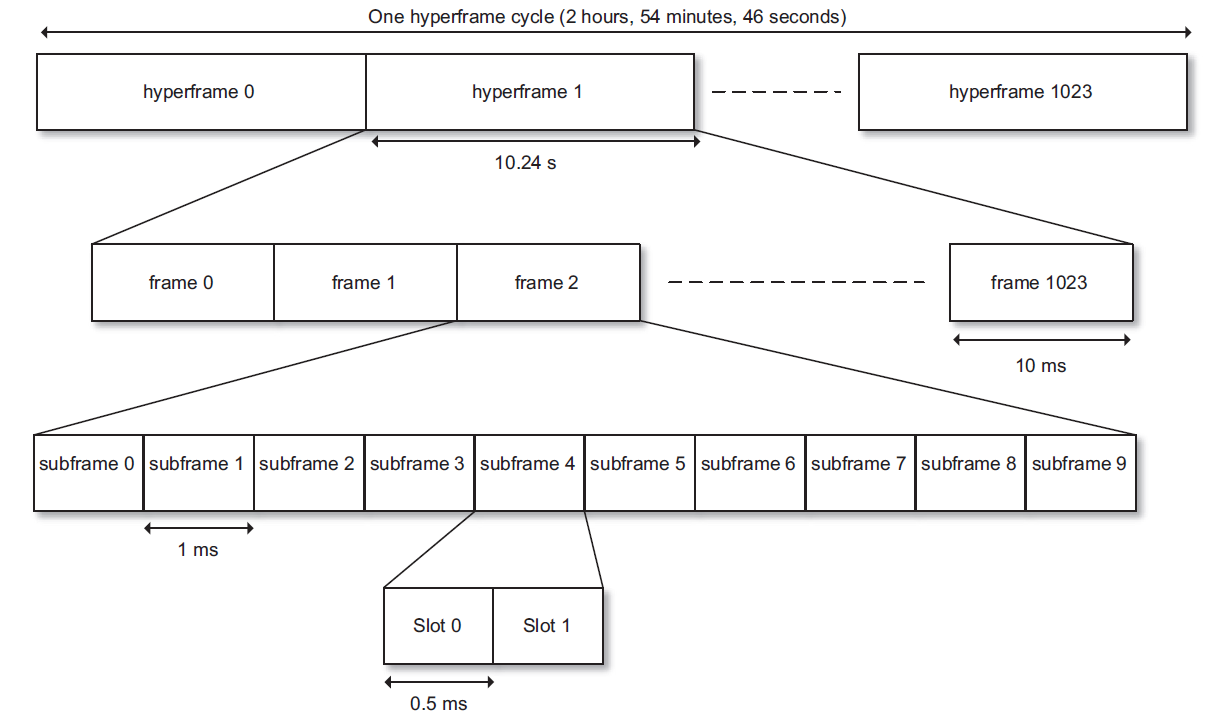
\includegraphics[width=\textwidth]{figures/downlink_structure_15kHz.png}
\caption{\gls{NB-IoT} downlink structure \citep[Fig. 7.7]{NB-IoT_Book}.}
\label{fig:downlink-structure}
\end{figure}


As the \gls{NB-IoT} system is placed outside the \gls{PRB}s used for LTE synchronization, most of the subframes are available to use, with the only exception being when a \gls{MBSFN} is present, which can occupy either of subframes (1,2,3,6,7,8) \citep{LTE-MBSFN}. Therefore the \gls{NPSS} and \gls{NSSS} is placed in subframe 5 and 9 respectively as seen on \autoref{fig:frame-structure}. By having the \gls{NSSS} being present only in even numbered frame, the \gls{LSB} of the frame numbers can be deduced directly. This increases the efficiency of the system by freeing subframe 9 in odd numbered frames and omitting that bit from the \gls{NB-IoT} overhead. The \gls{NPBCH} is located in the subframe 0 and contains the \gls{MIB-NB} \citep{REL-13}.  

\tikzsetnextfilename{frameStructure}
\begin{figure}[H]
\centering
\definecolor{NPSS}{HTML}{00D0FF}
\definecolor{NSSS}{HTML}{F97BFF}
\definecolor{NPBCH}{HTML}{92D050}
\usetikzlibrary{patterns,decorations.pathreplacing}

\resizebox{\textwidth}{!}{
\begin{tikzpicture}[scale = 0.4]

\draw [thick,decoration={brace,mirror,raise=0.1cm},decorate] (-20,-4) -- (-16,-4) node [pos=0.5,anchor=north,yshift=-0.1cm] {1 ms}; 
\draw [thick,decoration={brace,mirror,raise=0.2cm},decorate] (-20,-5) -- (20,-5) node [pos=0.5,anchor=north,yshift=-0.3cm] {10 ms};



\draw[fill = NPBCH]  (-20,2) rectangle (-16,0);
\draw  (-16,2) rectangle (-12,0);
\draw  (-12,2) rectangle (-8,0);
\draw  (-8,2) rectangle (-4,0);
\draw  (-4,2) rectangle (0,0);
\draw[fill = NPSS]  (0,2) rectangle (4,0);
\draw  (4,2) rectangle (8,0);
\draw  (8,2) rectangle (12,0);
\draw  (12,2) rectangle (16,0);
\draw[fill = NSSS]  (16,2) rectangle (20,0);

\draw[fill = NPBCH]  (-20,-2) rectangle (-16,-4);
\draw  (-16,-2) rectangle (-12,-4);
\draw  (-12,-2) rectangle (-8,-4);
\draw  (-8,-2) rectangle (-4,-4);
\draw  (-4,-2) rectangle (0,-4);
\draw[fill = NPSS]  (0,-2) rectangle (4,-4);
\draw  (4,-2) rectangle (8,-4);
\draw  (8,-2) rectangle (12,-4);
\draw  (12,-2) rectangle (16,-4);
\draw  (16,-2) rectangle (20,-4);

\node at (-18,3) {0};
\node at (-14,3) {1};
\node at (-10,3) {2};
\node at (-6,3) {3};
\node at (-2,3) {4};
\node at (2,3) {5};
\node at (6,3) {6};
\node at (10,3) {7};
\node at (14,3) {8};
\node at (18,3) {9};
\node at (-22,1) {even};
\node at (-22,-3) {odd};
\node [rotate = 90] at (-24,-1) {\textbf{Frame number}}; 

\node at (-18,1) {\acrshort{NPBCH}};
\node at (-18,-3) {\acrshort{NPBCH}};
\node at (2,1) {\acrshort{NPSS}};
\node at (2,-3) {\acrshort{NPSS}};
\node at (18,1) {\acrshort{NSSS}};
\node at (-14,1) {*};
\node at (-10,1) {*};
\node at (-6,1) {*};
\node at (-2,1) {*};
\node at (6,1) {*};
\node at (10,1) {*};
\node at (14,1) {*};
\node at (-14,-3) {*};
\node at (-10,-3) {*};
\node at (-6,-3) {*};
\node at (-2,-3) {*};
\node at (6,-3) {*};
\node at (10,-3) {*};
\node at (14,-3) {*};
\node at (18,-3) {*};
\node at (0,4.5) {\textbf{Subframe number}}; 

\node at (-15,-7) {* \acrshort{NPDCCH}/\acrshort{NPDSCH}};
\end{tikzpicture}
}

\caption{\gls{NB-IoT} frame structure \citep{REL-13}.}
\label{fig:frame-structure}
\end{figure}


By zooming in on a subframe, it is possible to see how the different \gls{OFDM} symbols is utilized. During a subframe, 14 \gls{OFDM} symbols are transmitted, each having 12 subcarriers, which results in 168 \gls{RE} per subframe. As can be seen on \autoref{fig:subframe-structure}, almost half of the \gls{RE} in a subframe might be reserved for different signals and \gls{LTE} control information \citep{REL-13}. An \gls{LTE} cell can allocate up to three symbols for \gls{PDCCH} and might use up to four carrier, which needs four \gls{RS}s \citep{whitepaper}. The \gls{NB-IoT} structure allows for up to two carriers and needs therefore two \gls{RS} namely \gls{NRS}1 and \gls{NRS}2 \citep{REL-13}. The placement of all these signals can be seen in \autoref{fig:subframe-structure}.  

\tikzsetnextfilename{subframe}
\begin{figure}[H]
\centering
\definecolor{LTERS}{HTML}{496d22}
\definecolor{LTECCH}{HTML}{92D050}
\definecolor{NPSS}{HTML}{00D0FF}
\definecolor{NSSS}{HTML}{F97BFF}


\resizebox{\textwidth}{!}{
\begin{tikzpicture}[scale=0.5]

\draw[pattern=north west lines, pattern color=LTECCH]  (-21,9) rectangle (-12,-9);
\draw [thick,decoration={brace,mirror},decorate] (-25.5,9) -- (-25.5,-9) node [pos=0.5,anchor=east, xshift=-0.1cm] {180 kHz};
\draw [thick,decoration={brace,mirror,raise=0.1cm},decorate] (-22.2,-7.5) -- (-22.2,-9) node [pos=0.5,anchor=east,xshift=-0.1cm] {15 kHz};
\draw [thick,decoration={brace,mirror,raise=0.1cm},decorate] (-21,-9.5) -- (-18,-9.5) node [pos=0.5,anchor=north,yshift=-0.2cm] {66.7 $\mu$ s};
\draw [thick,decoration={brace,mirror,raise=0.1cm},decorate] (-21,-11) -- (21,-11) node [pos=0.5,anchor=north,yshift=-0.2cm] {1 ms};


\node[text =red] at (-10.5,11) {Slot 0};
\node[text =red] at (10,11) {Slot 1};

%række 11
\draw  (-21,9) rectangle (-18,7.5);
\draw  (-18,9) rectangle (-15,7.5);
\draw  (-15,9) rectangle (-12,7.5);
\draw  (-12,9) rectangle (-9,7.5);
\draw  (-9,9) rectangle (-6,7.5);
\draw  (-6,9) rectangle (-3,7.5);
\draw  (-3,9) rectangle (0,7.5);
\draw  (-0,9) node (v1) {} rectangle (3,7.5);
\draw  (3,9) rectangle (6,7.5);
\draw  (6,9) rectangle (9,7.5);
\draw  (9,9) rectangle (12,7.5);
\draw  (12,9) rectangle (15,7.5);
\draw  (15,9) rectangle (18,7.5);
\draw  (18,9) rectangle (21,7.5);

%række 10
\draw  (-21,7.5) rectangle (-18,6);
\draw  (-18,7.5) rectangle (-15,6);
\draw  (-15,7.5) rectangle (-12,6);
\draw  (-12,7.5) rectangle (-9,6);
\draw  (-9,7.5) rectangle (-6,6);
\draw  (-6,7.5) rectangle (-3,6);
\draw  (-3,7.5) rectangle (0,6);
\draw  (-0,7.5) rectangle (3,6);
\draw  (3,7.5) rectangle (6,6);
\draw  (6,7.5) rectangle (9,6);
\draw  (9,7.5) rectangle (12,6);
\draw  (12,7.5) rectangle (15,6);
\draw  (15,7.5) rectangle (18,6);
\draw  (18,7.5) rectangle (21,6);

%række 9
\draw[pattern=north west lines, pattern color=LTERS] (-21,6) rectangle (-18,4.5);
\draw[pattern=north west lines, pattern color=LTERS] (-18,6) rectangle (-15,4.5);
\draw  (-15,6) rectangle (-12,4.5);
\draw  (-12,6) rectangle (-9,4.5);
\draw[pattern=north west lines, pattern color=LTERS]  (-9,6) rectangle (-6,4.5);
\draw[pattern=north west lines, pattern color=NSSS]  (-6,6) rectangle (-3,4.5);
\draw[pattern=north west lines, pattern color=NPSS]  (-3,6) rectangle (0,4.5);
\draw[pattern=north west lines, pattern color=LTERS]  (-0,6) rectangle (3,4.5);
\draw[pattern=north west lines, pattern color=LTERS]  (3,6) rectangle (6,4.5);
\draw  (6,6) rectangle (9,4.5);
\draw  (9,6) rectangle (12,4.5);
\draw[pattern=north west lines, pattern color=LTERS]  (12,6) rectangle (15,4.5);
\draw[pattern=north west lines, pattern color=NSSS] (15,6) rectangle (18,4.5);
\draw[pattern=north west lines, pattern color=NPSS]  (18,6) rectangle (21,4.5);

%række 8
\draw  (-21,4.5) rectangle (-18,3);
\draw  (-18,4.5) rectangle (-15,3);
\draw  (-15,4.5) rectangle (-12,3);
\draw  (-12,4.5) rectangle (-9,3);
\draw  (-9,4.5) rectangle (-6,3);
\draw  (-6,4.5) rectangle (-3,3);
\draw  (-3,4.5) rectangle (0,3);
\draw  (-0,4.5) rectangle (3,3);
\draw  (3,4.5) rectangle (6,3);
\draw  (6,4.5) rectangle (9,3);
\draw  (9,4.5) rectangle (12,3);
\draw  (12,4.5) rectangle (15,3);
\draw  (15,4.5) rectangle (18,3);
\draw  (18,4.5) rectangle (21,3);

%række 7
\draw  (-21,3) rectangle (-18,1.5);
\draw  (-18,3) rectangle (-15,1.5);
\draw  (-15,3) rectangle (-12,1.5);
\draw  (-12,3) rectangle (-9,1.5);
\draw  (-9,3) rectangle (-6,1.5);
\draw  (-6,3) rectangle (-3,1.5);
\draw  (-3,3) rectangle (0,1.5);
\draw  (-0,3) rectangle (3,1.5);
\draw  (3,3) rectangle (6,1.5);
\draw  (6,3) rectangle (9,1.5);
\draw  (9,3) rectangle (12,1.5);
\draw  (12,3) rectangle (15,1.5);
\draw  (15,3) rectangle (18,1.5);
\draw  (18,3) rectangle (21,1.5);

%række 6
\draw[pattern=north west lines, pattern color=LTERS] (-21,1.5) rectangle (-18,0);
\draw[pattern=north west lines, pattern color=LTERS] (-18,1.5) rectangle (-15,0);
\draw  (-15,1.5) rectangle (-12,0);
\draw  (-12,1.5) rectangle (-9,0);
\draw[pattern=north west lines, pattern color=LTERS]  (-9,1.5) rectangle (-6,0);
\draw[pattern=north west lines, pattern color=NPSS]  (-6,1.5) rectangle (-3,0);
\draw[pattern=north west lines, pattern color=NSSS]  (-3,1.5) rectangle (0,0);
\draw[pattern=north west lines, pattern color=LTERS]  (-0,1.5) rectangle (3,0);
\draw[pattern=north west lines, pattern color=LTERS]  (3,1.5) rectangle (6,0);
\draw  (6,1.5) rectangle (9,0);
\draw  (9,1.5) rectangle (12,0);
\draw[pattern=north west lines, pattern color=LTERS]  (12,1.5) rectangle (15,0);
\draw[pattern=north west lines, pattern color=NPSS]  (15,1.5) rectangle (18,0);
\draw[pattern=north west lines, pattern color=NSSS] (18,1.5) rectangle (21,0);

%række 5
\draw  (-21,-0) rectangle (-18,-1.5);
\draw  (-18,-0) rectangle (-15,-1.5);
\draw  (-15,-0) rectangle (-12,-1.5);
\draw  (-12,-0) rectangle (-9,-1.5);
\draw  (-9,-0) rectangle (-6,-1.5);
\draw  (-6,-0) rectangle (-3,-1.5);
\draw  (-3,-0) rectangle (0,-1.5);
\draw  (-0,-0) rectangle (3,-1.5);
\draw  (3,-0) rectangle (6,-1.5);
\draw  (6,-0) rectangle (9,-1.5);
\draw  (9,-0) rectangle (12,-1.5);
\draw  (12,-0) rectangle (15,-1.5);
\draw  (15,-0) rectangle (18,-1.5);
\draw  (18,-0) rectangle (21,-1.5);

%række 4
\draw  (-21,-1.5) rectangle (-18,-3);
\draw  (-18,-1.5) rectangle (-15,-3);
\draw  (-15,-1.5) rectangle (-12,-3);
\draw  (-12,-1.5) rectangle (-9,-3);
\draw  (-9,-1.5) rectangle (-6,-3);
\draw  (-6,-1.5) rectangle (-3,-3);
\draw  (-3,-1.5) rectangle (0,-3);
\draw  (-0,-1.5) rectangle (3,-3);
\draw  (3,-1.5) rectangle (6,-3);
\draw  (6,-1.5) rectangle (9,-3);
\draw  (9,-1.5) rectangle (12,-3);
\draw  (12,-1.5) rectangle (15,-3);
\draw  (15,-1.5) rectangle (18,-3);
\draw  (18,-1.5) rectangle (21,-3);

%række 3
\draw[pattern=north west lines, pattern color=LTERS] (-21,-3) rectangle (-18,-4.5);
\draw[pattern=north west lines, pattern color=LTERS] (-18,-3) rectangle (-15,-4.5);
\draw  (-15,-3) rectangle (-12,-4.5);
\draw  (-12,-3) rectangle (-9,-4.5);
\draw[pattern=north west lines, pattern color=LTERS]  (-9,-3) rectangle (-6,-4.5);
\draw[pattern=north west lines, pattern color=NSSS]  (-6,-3) rectangle (-3,-4.5);
\draw[pattern=north west lines, pattern color=NPSS]  (-3,-3) rectangle (0,-4.5);
\draw[pattern=north west lines, pattern color=LTERS]  (-0,-3) rectangle (3,-4.5);
\draw[pattern=north west lines, pattern color=LTERS]  (3,-3) rectangle (6,-4.5);
\draw  (6,-3) rectangle (9,-4.5);
\draw  (9,-3) rectangle (12,-4.5);
\draw[pattern=north west lines, pattern color=LTERS]  (12,-3) rectangle (15,-4.5);
\draw[pattern=north west lines, pattern color=NSSS]  (15,-3) rectangle (18,-4.5);
\draw[pattern=north west lines, pattern color=NPSS]  (18,-3) rectangle (21,-4.5);

%række 2
\draw  (-21,-4.5) rectangle (-18,-6);
\draw  (-18,-4.5) rectangle (-15,-6);
\draw  (-15,-4.5) rectangle (-12,-6);
\draw  (-12,-4.5) rectangle (-9,-6);
\draw  (-9,-4.5) rectangle (-6,-6);
\draw  (-6,-4.5) rectangle (-3,-6);
\draw  (-3,-4.5) rectangle (0,-6);
\draw  (-0,-4.5) rectangle (3,-6);
\draw  (3,-4.5) rectangle (6,-6);
\draw  (6,-4.5) rectangle (9,-6);
\draw  (9,-4.5) rectangle (12,-6);
\draw  (12,-4.5) rectangle (15,-6);
\draw  (15,-4.5) rectangle (18,-6);
\draw  (18,-4.5) rectangle (21,-6);

%række 1
\draw  (-21,-6) rectangle (-18,-7.5);
\draw  (-18,-6) rectangle (-15,-7.5);
\draw  (-15,-6) rectangle (-12,-7.5);
\draw  (-12,-6) rectangle (-9,-7.5);
\draw  (-9,-6) rectangle (-6,-7.5);
\draw  (-6,-6) rectangle (-3,-7.5);
\draw  (-3,-6) rectangle (0,-7.5);
\draw  (-0,-6) rectangle (3,-7.5);
\draw  (3,-6) rectangle (6,-7.5);
\draw  (6,-6) rectangle (9,-7.5);
\draw  (9,-6) rectangle (12,-7.5);
\draw  (12,-6) rectangle (15,-7.5);
\draw  (15,-6) rectangle (18,-7.5);
\draw  (18,-6) rectangle (21,-7.5);

%række 0
\draw[pattern=north west lines, pattern color=LTERS] (-21,-7.5) rectangle (-18,-9);
\draw[pattern=north west lines, pattern color=LTERS] (-18,-7.5) rectangle (-15,-9);
\draw  (-15,-7.5) rectangle (-12,-9); 
\draw  (-12,-7.5) rectangle (-9,-9);
\draw[pattern=north west lines, pattern color=LTERS]  (-9,-7.5) rectangle (-6,-9);
\draw[pattern=north west lines, pattern color=NPSS]  (-6,-7.5) rectangle (-3,-9);
\draw[pattern=north west lines, pattern color=NSSS]  (-3,-7.5) rectangle (0,-9) node (v2) {};
\draw[pattern=north west lines, pattern color=LTERS]  (-0,-7.5) rectangle (3,-9);
\draw[pattern=north west lines, pattern color=LTERS]  (3,-7.5) rectangle (6,-9);
\draw  (6,-7.5) rectangle (9,-9);
\draw  (9,-7.5) rectangle (12,-9);
\draw[pattern=north west lines, pattern color=LTERS]  (12,-7.5) rectangle (15,-9);
\draw[pattern=north west lines, pattern color=NPSS]  (15,-7.5) rectangle (18,-9);
\draw[pattern=north west lines, pattern color=NSSS]  (18,-7.5) rectangle (21,-9);


\node at (-22,-8.25) {0};
\node at (-22,-6.75) {1};
\node at (-22,-5.25) {2};
\node at (-22,-3.75) {3};
\node at (-22,-2.25) {4};
\node at (-22,-0.75) {5};
\node at (-22,0.75) {6};
\node at (-22,2.25) {7};
\node at (-22,3.75) {8};
\node at (-22,5.25) {9};
\node at (-22,6.75) {10};
\node at (-22,8.25) {11};

\node at (-19.5,10) {0};
\node at (-16.5,10) {1};
\node at (-13.5,10) {2};
\node at (-10.5,10) {3};
\node at (-7.5,10) {4};
\node at (-4.5,10) {5};
\node at (-1.5,10) {6};
\node at (1.5,10) {7};
\node at (4.5,10) {8};
\node at (7.5,10) {9};
\node at (10.5,10) {10};
\node at (13.5,10) {11};
\node at (16.5,10) {12};
\node at (19.5,10) {13};

\draw[draw=red,line width=2pt] (0,9) -- (0,-9);
\draw[pattern=north west lines, pattern color=LTERS]  (-21,-13) rectangle (-18,-14.5);
\draw[pattern=north west lines, pattern color=LTECCH]  (-13,-13) rectangle (-10,-14.5);
\draw[pattern=north west lines, pattern color=NPSS]  (-3.5,-13) rectangle (-0.5,-14.5) ;
\draw[pattern=north west lines, pattern color=NSSS]  (4,-13) rectangle (7,-14.5) ;
\draw (11.5,-13) rectangle (14.5,-14.5);

\node[anchor=west] at (-17.5,-13.75) {\acrshort{LTE} \acrshort{RS}};
\node[anchor=west] at (-9.5,-13.75) {\acrshort{LTE} \acrshort{PDCCH}};
\node[anchor=west] at (-0,-13.75) {\acrshort{NRS}1};
\node[anchor=west] at (7.5,-13.75) {\acrshort{NRS}2};
\node[anchor=west] at (15,-13.75) {Free symbol};

\end{tikzpicture}
}
\caption{The structure of a \gls{DL} subframe \citep{whitepaper,REL-13}.}
\label{fig:subframe-structure}
\end{figure}

It should be noted that the described allocation is a worst case scenario for the \gls{DL}. If the system is deployed either in guard-band or as stand-alone, only the \gls{NRS} is actually used, but before the device is synchronized, it does not know what is in use and needs to guard for this worst case scenario. When the device receives the \gls{MIB-NB} and \gls{NB-SIB}1 it will get information in regards to the number of carriers and the size of \gls{LTE} \gls{PDCCH} \citep{whitepaper}. 

Channels\\ 
As shown on \autoref{fig:frame-structure}, three channels exist in the physical \gls{DL} part of the protocol. These are respectively: \gls{NPBCH}, \gls{NPDCCH} and \gls{NPDSCH}. The structure of the \gls{NPBCH} is explained in the \autoref{sec:Network_access}.

The \gls{NPDCCH} carries three types of information: one is use to indicate \gls{DL} scheduling for the devices, one provides \gls{UL} grant information and the last indicates paging or system information update \citep{NB-IoT_Book}. It should be noted that  depending on the coverage level the \gls{NPDCCH} might be repeated up 2048 times \citep{NB-IoT_Book}.

The \gls{NPDSCH} is used to transmit data when an bearer is established. Depending on the coverage level the \gls{NPDSCH} might be repeated up 2048 times. A \gls{TBS} may be up to 680 bits depending on the \gls{TBS} index and the number of subframes used. \citep{NB-IoT_Book}

\subsubsection{Uplink}
\label{sec:ULphy}
As mentioned in \autoref{ch:Introduction}, most of the data in the system is \gls{UL} data. Therefore is the \gls{UL} spectrum tuned to accommodate the massive number of devices. The timing alignment of the \gls{UL} follows the \gls{DL} meaning when synchronized to the \gls{DL} band, the device is also synchronized to the \gls{UL}, except for the delay introduced by the travelling time of the signal. This delay is found at the beginning of the \gls{RAP}, which will be further explained in \autoref{sec:RAP}. 

Frame Structure\\
Compared to legacy \gls{LTE}, two differences should be noted. The channel \gls{PUCCH} has been removed and the \gls{UL} frame can take different formats. It is 180 kHz wide, as the \gls{DL} frame, however the sub carrier spacing can be both 3.75 kHz and 15 kHz, giving 48 and 12 subcarriers respectively. This is however only done on the \gls{NPUSCH}, in the \gls{NPRACH} the subcarrier spacing is always 3.75 kHz \citep{NB-IoT_Book}. For each symbol that is transmitted, a \gls{CP} is used. The structure of the channels can be seen on \autoref{fig:NPUSCH1_structure}, \autoref{fig:NPUSCH2_structure} and \autoref{fig:NPRACH_structure}.

\begin{minipage}{0.48\textwidth}
\begin{figure}[H]
\centering
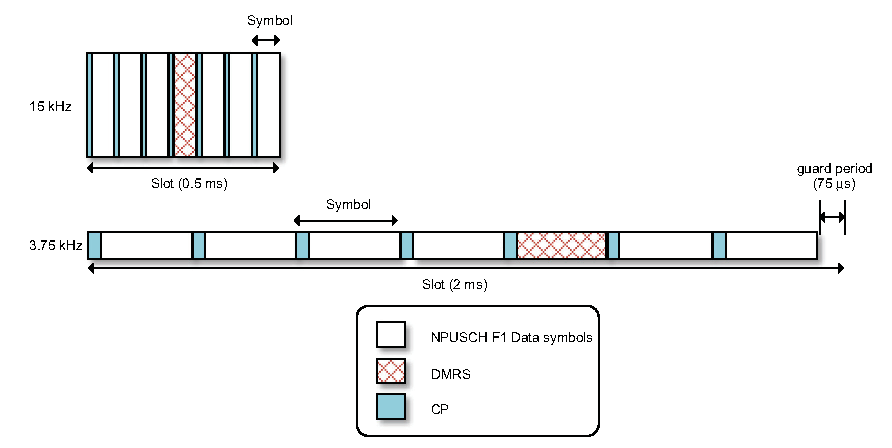
\includegraphics[width=\textwidth]{figures/NPUSCH1_structure.pdf}
\caption{The structure of NPUSCH format 1 \citep{NB-IoT_Book}}
\label{fig:NPUSCH1_structure}
\end{figure}
\end{minipage}%
\hfill
\begin{minipage}{0.48\textwidth}
\begin{figure}[H]
\centering
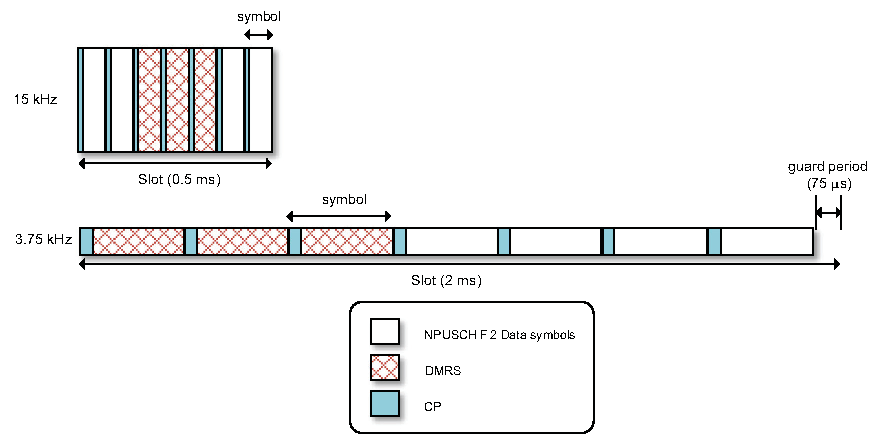
\includegraphics[width=\textwidth]{figures/NPUSCH2_structure.pdf}
\caption{The structure of NPUSCH format 2 \citep{NB-IoT_Book}}
\label{fig:NPUSCH2_structure}
\end{figure}
\end{minipage}


\begin{figure}[H]
\centering
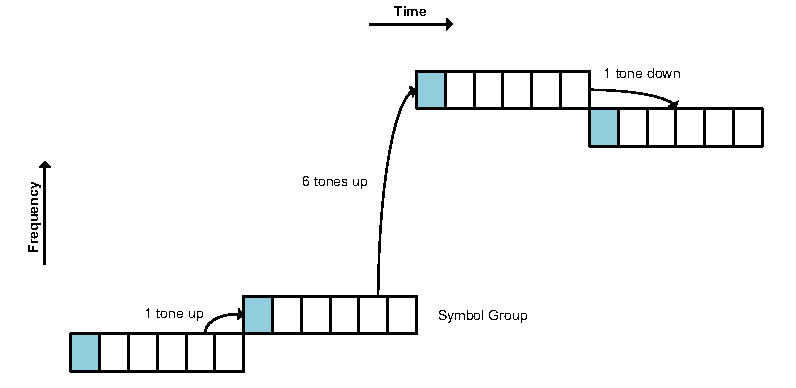
\includegraphics[width=0.5\textwidth]{figures/NPRACH_frequency_hopping.pdf}
\caption{The structure of a NPRACH symbol group \citep{NB-IoT_Book}}
\label{fig:NPRACH_structure}
\end{figure}

Channels\\
The \gls{UL} consists of two channels and one signal, namely the \gls{NPRACH}, \gls{NPUSCH} and \gls{DMRS}.

The \gls{NPRACH} consist of a repetition of four symbol groups, for each symbol group a \gls{CP} is attached followed by five symbols. The duration of the CP is dependent on the CP-format chosen this can be seen in \autoref{fig:NPRACH_structure}, and depending on the coverage level the \gls{NPRACH} might be repeated up to 128 times. The NPRACH only uses 12 subcarriers at any time, which are used for msg1 in the \gls{NRAP}, see \autoref{sec:RAP}. \citep{NB-IoT_Book}

The \gls{NPUSCH} carries the data transmitted form the device and \gls{HARQ} acknowledgement from the \gls{NPDSCH}, this is referred to as format 1 and 2 respectively. Format 1 can carry up 1000 bits per \gls{TB}. As seen on \autoref{fig:NPUSCH1_structure} and \autoref{fig:NPUSCH2_structure} the DMRS, which is used for channel estimation at the base station, is multiplexed with the NPUSCH. 






\section{Network Access}
\label{sec:Network_access}
This section describes the different procedures needed to navigate in the NB-IoT framework. This is the procedure to establish a connection as well as the procedures to navigate between different connection states. 

\subsection{Cell Search and Synchronization Procedure}
\label{sec:cellsync}
The first thing needed of a device is to locate a cell, this is done during the as part of the synchronization procedure. The synchronization procedure is very similar to that of a \gls{LTE} as can be seen in \autoref{fig:sync-NB}, as the device first needs to search for the cell and then acquire the system information. 


\tikzsetnextfilename{sync-NB}
\begin{figure}[H]
\centering
\definecolor{top}{HTML}{00FFFF}
\definecolor{center}{HTML}{0080FF}
\definecolor{bund}{HTML}{0000FF}
\usetikzlibrary{arrows}

%\resizebox{0.5\textwidth}{!}{
\begin{tikzpicture}[scale = 0.4]

\draw (-7.5,8) rectangle (-2.5,6);
\node at (-5,7) {Device};
\draw [dashed] (-5,6) -- (-5,-4);

\draw (2.5,8) rectangle (7.5,6);
\node at (5,7) {\acrshort{eNB}};
\draw [dashed] (5,6) -- (5,-4);

\draw[arrows={triangle 45-}] (-5,4) -- (5,4);
\node at (0,4.5) {\acrshort{NPSS}};

\draw[arrows={triangle 45-}] (-5,2) -- (5,2);
\node at (0,2.5) {\acrshort{NSSS}};

\draw[arrows={triangle 45-}] (-5,0) -- (5,0);
\node at (0,0.5) {\acrshort{MIB-NB}};

\draw[arrows={triangle 45-}] (-5,-2) -- (5,-2);
\node at (0,-1.5) {\acrshort{NB-SIB}s};

\end{tikzpicture}
%}

\caption{The process needed to synchronize to a cell.}
\label{fig:sync-NB}
\end{figure}

The device first looks for the \gls{NPSS}, the search spaces for the \gls{NPSS} is predetermined based on the LTE bands. \todo{make ref to LTE bands} This provides the initial \gls{CFO} as well as a 10 ms timing alignment. As mentioned the NPSS takes up the entire fifth subframe of each frame, a frequency domain Zadoff-Chu sequence is used for the 11 available \gls{OFDM} symbols, as the first 3 OFDM might be used for LTE PDCCH. For low complexity devices a single 10 ms segment might not suffice at a low \gls{SNR}, the structure of the \gls{NPSS} is therefore made so the signals can accumulate coherently over multiple 10 ms segments. \citep{NB-IoT_Book,primer}. The \gls{NSSS} is also based on a frequency domain Zadoff-Chu sequence, but is further scrambled based on the \gls{NB-PCID}. This means the device has to manually try each frequency and then manually test for each of the 504 NB-PCID. When this is done the device will be frequency and in a 80 ms window time synchronized with the eNB and know the NB-PCID also \citep{NB-IoT_Book,primer}. 

The next step is to decode the \gls{MIB-NB}, it consists of 34 bits and 16 \gls{CRC} bits, they are transmitted in eight self-decodeable blocks which is repeated eight times resulting in a total transmission time of 640 ms as can be seen on \autoref{fig:MIB-NB}. 
 
\tikzsetnextfilename{MIB-NB}
\begin{figure}[H]
\centering
\definecolor{top}{HTML}{00FFFF}
\definecolor{center}{HTML}{0080FF}
\definecolor{bund}{HTML}{0000FF}
\usetikzlibrary{arrows}

\resizebox{\textwidth}{!}{
\begin{tikzpicture}[scale = 0.4]

\draw [fill=top] (-20,8) rectangle (20,6);
\node at (0,7) {\acrshort{MIB-NB}};
\draw (-20,10) -- (-20,8);
\draw (20,10) -- (20,8);
\node (top) at (0,9) {640 ms};
\draw[arrows={-triangle 45}] (top) edge (-20,9);
\draw[arrows={-triangle 45}] (top) edge (20,9);

\draw (0,6) -- (0,4); 
\draw (-17.5,4) -- (17.5,4);

\draw[arrows={-triangle 45}] (-17.5,4) -- (-17.5,2);
\draw[arrows={-triangle 45}] (-12.5,4) -- (-12.5,2);
\draw[arrows={-triangle 45}] (-7.5,4) -- (-7.5,2);
\draw[arrows={-triangle 45}] (-2.5,4) -- (-2.5,2);
\draw[arrows={-triangle 45}] (2.5,4) -- (2.5,2);
\draw[arrows={-triangle 45}] (7.5,4) -- (7.5,2);
\draw[arrows={-triangle 45}] (12.5,4) -- (12.5,2);
\draw[arrows={-triangle 45}] (17.5,4) -- (17.5,2);

\draw [fill=center] (-20,2) rectangle (-15,0);
\draw [fill=center] (-15,2) rectangle (-10,0);
\draw [fill=center] (-10,2) rectangle (-5,0);
\draw [fill=center] (-5,2) rectangle (0,0);
\draw [fill=center] (0,2) rectangle (5,0);
\draw [fill=center] (5,2) rectangle (10,0);
\draw [fill=center] (10,2) rectangle (15,0);
\draw [fill=center] (15,2) rectangle (20,0);

\node at (-17.5,1) {BL1};
\node at (-12.5,1) {BL2};
\node at (-7.5,1) {BL3};
\node at (-2.5,1) {BL4};
\node at (2.5,1) {BL5};
\node at (7.5,1) {BL6};
\node at (12.5,1) {BL7};
\node at (17.5,1) {BL8};

\node(bl1) at (-17.5,-1) {80 ms};
\draw[arrows={-triangle 45}] (bl1) edge (-20,-1);
\draw[arrows={-triangle 45}] (bl1) edge (-15,-1);
\draw (-15,0) -- (-15,-2);
\draw (-20,0) -- (-20,-4);
\draw (-15,-2) -- (20,-4);

\draw [fill=bund] (-20,-4) rectangle (-19.5,-6);
\draw [fill=bund] (-15,-4) rectangle (-14.5,-6);
\draw [fill=bund] (-10,-4) rectangle (-9.5,-6);
\draw [fill=bund] (-5,-4) rectangle (-4.5,-6);
\draw [fill=bund] (0,-4) rectangle (0.5,-6);
\draw [fill=bund] (5,-4) rectangle (5.5,-6);
\draw [fill=bund] (10,-4) rectangle (10.5,-6);
\draw [fill=bund] (15,-4) rectangle (15.5,-6);

\draw (-19.5,-4) rectangle (-19,-6);
\draw (-19,-4) rectangle (-18.5,-6);
\draw (-18.5,-4) rectangle (-18,-6);
\draw (-18,-4) rectangle (-17.5,-6);
\draw (-17.5,-4) rectangle (-17,-6);
\draw (-17,-4) rectangle (-16.5,-6);
\draw (-16.5,-4) rectangle (-16,-6);
\draw (-16,-4) rectangle (-15.5,-6);
\draw (-15.5,-4) rectangle (-15,-6);

\draw (-14.5,-4) rectangle (-14,-6);
\draw (-14,-4) rectangle (-13.5,-6);
\draw (-13.5,-4) rectangle (-13,-6);
\draw (-13,-4) rectangle (-12.5,-6);
\draw (-12.5,-4) rectangle (-12,-6);
\draw (-12,-4) rectangle (-11.5,-6);
\draw (-11.5,-4) rectangle (-11,-6);
\draw (-11,-4) rectangle (-10.5,-6);
\draw (-10.5,-4) rectangle (-10,-6);

\draw (-9.5,-4) rectangle (-9,-6);
\draw (-9,-4) rectangle (-8.5,-6);
\draw (-8.5,-4) rectangle (-8,-6);
\draw (-8,-4) rectangle (-7.5,-6);
\draw (-7.5,-4) rectangle (-7,-6);
\draw (-7,-4) rectangle (-6.5,-6);
\draw (-6.5,-4) rectangle (-6,-6);
\draw (-6,-4) rectangle (-5.5,-6);
\draw (-5.5,-4) rectangle (-5,-6);

\draw (-4.5,-4) rectangle (-4,-6);
\draw (-4,-4) rectangle (-3.5,-6);
\draw (-3.5,-4) rectangle (-3,-6);
\draw (-3,-4) rectangle (-2.5,-6);
\draw (-2.5,-4) rectangle (-2,-6);
\draw (-2,-4) rectangle (-1.5,-6);
\draw (-1.5,-4) rectangle (-1,-6);
\draw (-1,-4) rectangle (-0.5,-6);
\draw (-0.5,-4) rectangle (-0,-6);

\draw (0.5,-4) rectangle (1,-6);
\draw (1,-4) rectangle (1.5,-6);
\draw (1.5,-4) rectangle (2,-6);
\draw (2,-4) rectangle (2.5,-6);
\draw (2.5,-4) rectangle (3,-6);
\draw (3,-4) rectangle (3.5,-6);
\draw (3.5,-4) rectangle (4,-6);
\draw (4,-4) rectangle (4.5,-6);
\draw (4.5,-4) rectangle (5,-6);

\draw (5.5,-4) rectangle (6,-6);
\draw (6,-4) rectangle (6.5,-6);
\draw (6.5,-4) rectangle (7,-6);
\draw (7,-4) rectangle (7.5,-6);
\draw (7.5,-4) rectangle (8,-6);
\draw (8,-4) rectangle (8.5,-6);
\draw (8.5,-4) rectangle (9,-6);
\draw (9,-4) rectangle (9.5,-6);
\draw (9.5,-4) rectangle (10,-6);

\draw (10.5,-4) rectangle (11,-6);
\draw (11,-4) rectangle (11.5,-6);
\draw (11.5,-4) rectangle (12,-6);
\draw (12,-4) rectangle (12.5,-6);
\draw (12.5,-4) rectangle (13,-6);
\draw (13,-4) rectangle (13.5,-6);
\draw (13.5,-4) rectangle (14,-6);
\draw (14,-4) rectangle (14.5,-6);
\draw (14.5,-4) rectangle (15,-6);

\draw (15.5,-4) rectangle (16,-6);
\draw (16,-4) rectangle (16.5,-6);
\draw (16.5,-4) rectangle (17,-6);
\draw (17,-4) rectangle (17.5,-6);
\draw (17.5,-4) rectangle (18,-6);
\draw (18,-4) rectangle (18.5,-6);
\draw (18.5,-4) rectangle (19,-6);
\draw (19,-4) rectangle (19.5,-6);
\draw (19.5,-4) rectangle (20,-6);

\end{tikzpicture}
}

\caption{MIB-NB}
\label{fig:MIB-NB}
\end{figure}

The information carried in the \gls{MIB-NB} are:

\begin{tabular}{ll}\\
2 bits & hyper frame number\\
4 bits & \gls{SFN}\\
4 bits & \gls{NB-SIB}1 scheduling\\
5 bits & value tag\\
1 bit & access barrer\\
7 bits & operation mode and values\\
11 bits & reserved for future use\\
\end{tabular}

From the \gls{MIB-NB} the schedule for \gls{NB-SIB}1 is found, this is always transmitted in subframe 4 however only the frames indicated by \gls{MIB-NB} carry \gls{NB-SIB}1. The final step in the synchronization is to decode all the \gls{NB-SIB}s.

When the device have read all \gls{NB-SIB}s it has fully synchronized with the \gls{eNB}. It is mandatory for the device to have a valid version of \gls{MIB-NB} as well as \gls{NB-SIB}1-5, \gls{NB-SIB}14 and 16 is only read when required. Furthermore once connected to the system the device is not expected to update its version of the \gls{NB-SIB}s unless instructed to \citep{whitepaper}. 

When the device is synchronized it can initiate the attach procedure which will now be described. 




\subsection{Narrowband Attach Procedure} \label{sec:RAP}
Before starting the narrowband attach procedure the device measures the reference signals and determine based and some \gls{RSRP} thresholds which coverage level should be applied. The coverage level determines the power level used as well as the number of repetition used \citep{NB-IoT_Book}. The narrowband attach procedure comes in three forms, a full attach where a connection is established and all the security modes and authentication happens, a connection resume where the previously established security is used and an establishment carrying data. Each form contains some smaller steps, but can generally be divided into: \gls{NRAP} and security establishment \citep{REL-13}. The security establishment follows the same pattern as LTE and will not be further explained. The \gls{NRAP} contain five messages:
\begin{tabular}{ll}
msg1 & is the NPRACH that can happen when a NPRACH occasion exists \\
msg2 & is the \gls{RAR} informing the device of timing offsets and providing a grant for msg3 \\
msg3 & is the connection request or connection resume request \\
msg4 & is contention resolution and acknowledgement of the request \\
msg5 & is the connection establishment complete message\\
\end{tabular}

This process can also be seen on \autoref{fig:RAP}


\tikzsetnextfilename{RAP}
\begin{figure}[H]
\centering
\usetikzlibrary{arrows}

\begin{tikzpicture}[scale = 0.4]

\draw (-13.5,8) rectangle (-8.5,6);
\node at (-11,7) {Device};
\draw [dashed] (-11,6) -- (-11,-4);

\draw (8.5,8) rectangle (13.5,6);
\node at (11,7) {eNB};
\draw [dashed] (11,6) -- (11,-4);

\draw[arrows={-triangle 45}] (-11,4) -- (11,4);
\node at (0,4.5) {NPRACH (msg1)};

\draw[arrows={triangle 45-}] (-11,2) -- (11,2);
\node at (0,2.5) {RAR (msg2)};

\draw[arrows={-triangle 45}] (-11,0) -- (11,0);
\node at (0,0.5) {RRC Connection Resume Request (msg3)};

\draw[arrows={triangle 45-}] (-11,-2) -- (11,-2);
\node at (0,-1.5) {RRC Connection Resume (msg4)};

\draw[arrows={-triangle 45}] (-11,-4) -- (11,-4);
\node at (0,-3.5) {RRC Connection Resume Complete (msg5)};
\end{tikzpicture}
\caption{Message visualisation of the \gls{RAP} for connection resume.}
\label{fig:RAP}
\end{figure}

The important parts to take from this is that the device gets a \gls{Ra-RNTI} based on the preamble it selects for msg1. This identifier is used to decode the rest of the messages. During the attach procedure the device is also given a \gls{P-RNTI} and a \gls{C-RNTI}, which is used for decoding radio and paging transmission later on \citep{whitepaper}. If a control plane data transmission is desired it is transmitted during the \gls{NRAP} \citep{primer}.


\subsection{Connection Control}
A connected device needs to be able to move around the different device states as seen in \autoref{fig:UE-states}. To do this different procedures is used. The primary concern here is moving in and out of idle modes, generally when connected, a device does not want to give up on its \gls{C-RNTI} as this makes the attach sequence significantly longer, that is where control plane optimization comes in. The control plane optimization enables the device to save its \gls{AS} when it goes in idle mode, this \gls{AS} is then used again when the device resumes the connection, this feature is utilized whenever possible. 

Another important aspect is the idle modes, this is where a device is expected to spend most of its time so the power consumption here needs to be minimal. The two primary idle modes are \gls{eDRX} and \gls{PSM}, however in both modes a period of time is spent in normal DRX mode. 


\subsubsection{DRX}
When the device wants to disconnect from the network it might be required to listen for mobile terminated data, this is done through the paging channel. The DRX cycle consist of a paging opportunity and a DRX opportunity, this can be seen in \autoref{fig:DRX_structure}. 

%\tikzsetnextfilename{DRX_structure}
\begin{figure}[H]
\centering
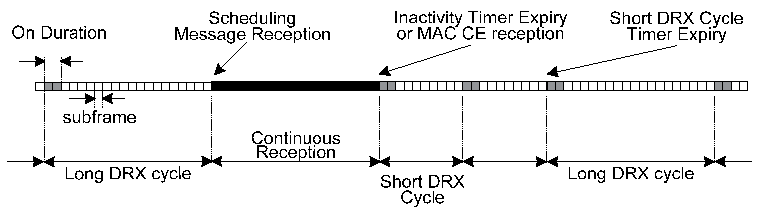
\includegraphics[width=\textwidth]{figures/DRX_structure.pdf}
\caption{The structure of \gls{DRX} idle mode \citep{book_LTE_for_UMTS2}}
\label{fig:DRX_structure}
\end{figure}

As seen on \autoref{fig:DRX_structure} several parameters define the DRX structure, the different parameters use and typical values can be found in \autoref{tab:DRX_parameters}

\begin{table}[H]
\centering
\begin{tabular}{|c|p{6cm}|p{4cm}|} \hline
\textbf{Parameter} & \textbf{Definition} & \textbf{Typical value} \\ \hline 
On duration &  the number of subframes that is monitored during the paging opportunity & 1-2 subframes\\ \hline
DRX inactivity timer & the period after a scheduling message where the device should be in continuous reception mode & 25-50 subframes \\ \hline
DRX short cycle timer & the duration of the short DRX cycle & 20-40 subframes \\ \hline
Retransmission timer & the period after a \gls{HARQ} round trip time in which the device needs to monitor the control channel & 20  subframes \\ \hline
Long DRX cycle & the duration of the short DRX cycle & 1024 subframes \\ \hline
\end{tabular}
\caption{The different parameters and their typical value when defining the DRX structure \citep{book_LTE_for_UMTS}.}
\label{tab:DRX_parameters}
\end{table}

It should be noted that these typical values are based on the DRX of LTE in NB-IoT it is uncertain if the short cycle would be used at all, and the long cycle might be as long as 10240 subframes. It is also important to note that contrary to LTE NB-IoT supports repetition of the NPDCCH channel which directly influences the paging messages. \citep{NB-IoT_Book}


\subsubsection{eDRX}
The eDRX idle mode is an extension of the DRX idle mode. It is designed to accommodate a medium length transmission interval. The build up consist of a long DRX opportunity followed by a normal DRX period often referred to as \gls{PTW}. During the long DRX opportunity only the necessary timers and PLL's to keep synchronize with the network is on, there is no need to listen to the NPDCCH for incoming data. In the \gls{PTW} the device returns to a normal DRX cycle structure and monitors the paging opportunities. This cycle can be seen on \autoref{fig:eDRX_structure}.

\tikzsetnextfilename{eDRX_structure}
\begin{figure}[H]
\centering
\resizebox{\textwidth}{!}{
\begin{tikzpicture}

\draw[dashed] (-10,1.5) -- (-1,1.5);
\draw[dashed] (1,1.5) -- (10,1.5);


\draw[dashed] (-10,0) -- (-1,0) node (v4) {};
\draw[dashed] (1,0) node (v5) {} -- (10,0) node (v8) {};
\draw (0,1.5) -- (-0.5,1) -- (0,0.5) -- (-0.5,0);
\draw (0.5,1.5) -- (0,1) -- (0.5,0.5) -- (0,0);
\node at (-10,1.5) {};
\node[anchor=east] at (-10,1.5) {RX:};
\node[anchor=east] (v1) at (-10,0) {Sleep:};
\draw (v1) -- (-9,0) -- (-9,1.5) -- (-8.5,1.5) -- (-8.5,0) node (v2) {};
\draw (v2) -- (-7.5,0) -- (-7.5,1.5) -- (-7,1.5) -- (-7,0) node (v3) {};
\draw (v3) -- (-6,0) -- (-6,1.5) -- (-5.5,1.5) -- (-5.5,0) -- (v4);
\draw (v5) -- (6,0) -- (6,1.5) -- (6.5,1.5) -- (6.5,0) node (v6) {};
\draw (v6) -- (7.5,0) -- (7.5,1.5) -- (8,1.5) -- (8,0) node (v7) {};
\draw (v7) -- (9,0) -- (9,1.5) -- (9.5,1.5) -- (9.5,0) -- (v8);

\draw[arrows={triangle 45- triangle 45}] (-9,-0.5) -- (-7.5,-0.5);
\draw[arrows={triangle 45- triangle 45}] (-9,-1.5) -- (-5.5,-1.5) ;
\draw[arrows={triangle 45- triangle 45}] (-9,-2.5) -- (6,-2.5);
\node at (-8.25,-1) {DRX cycle};
\node at (-7.25,-2) {PTW};
\node at (-1.5,-3) {eDRX cycle};
\end{tikzpicture}}
\caption{The structure of the \gls{eDRX} cycle}
\label{fig:eDRX_structure}
\end{figure}

A few parameters helps define this cycle, the first is the eDRX cycle the next is the duration of the \gls{PTW}. Supported values for these parameters can be seen in \autoref{tab:eDRX_parameters}.

\begin{table}[H]
\centering
\begin{tabular}{|c|p{8cm}|} \hline
\textbf{Parameter} & \textbf{Values in seconds} \\ \hline 
PTW & 2.56, 5.12, 7.68, 10.24, 12.8, 15.36, 17.92, 20.48, 23.04, 25.6, 28.16, 30.72, 33.28, 35.84, 38.40 and 40.96\\ \hline
eDRX cycle & 20.48, 40.96, 81.92, 163.84, 327.68, 655.36, 1310.72, 2621.44, 5242.88 and 10485.76 \\ \hline
\end{tabular}
\caption{The different parameters and their typical value when defining the DRX structure \citep{book_LTE_for_UMTS}.}
\label{tab:eDRX_parameters}
\end{table}

\subsubsection{PSM}
The PSM mode is designed to support long transmission intervals, a DRX period starts the PSM mode followed by the PSM state. While in the PSM state the device is only required to maintain its real time clock nothing else, this means that whenever the device wants to reconnect to the network it first needs to synchronize itself again. A timer is set when the device enters PSM mode, this timer defines when the device needs to wake up and perform a \gls{TAU}. This is to keep track of if a device has change location since it last connected to the network. After a TAU the device enters a DRX period again to enable mobile terminated data transmission. The structure of a PSM cycle can be seen in \autoref{fig:PSM_structure}.

\tikzsetnextfilename{PSM_structure}
\begin{figure}[H]
\centering
\resizebox{\textwidth}{!}{
\begin{tikzpicture}

\draw[dashed] (-10,3) -- (-1,3);
\draw[dashed] (1,3) -- (10,3);

\draw[dashed] (-10,1.5) -- (-1,1.5);
\draw[dashed] (1,1.5) -- (10,1.5);

\draw[dashed] (-10,0) -- (-1,0) node (v4) {};
\draw[dashed] (1,0) node (v5) {} -- (10,0) node (v8) {};

\draw (-0.0157,2.2353) -- (-0.5157,1.7353) -- (-0.0157,1.2353) -- (-0.5157,0.7353);
\draw (0.4843,2.2353) -- (-0.0157,1.7353) -- (0.4843,1.2353) -- (-0.0157,0.7353);

\node[anchor=east] at (-10,3) {TX:};
\node[anchor=east] at (-10,1.5) {RX:};
\node[anchor=east] (v1) at (-10,0) {Sleep:};

\draw (v1) -- (-9,0) -- (-9,3) -- (-7.5,3) -- (-7.5,0) node (v2) {};
\draw (v2) -- (-6.5,0) -- (-6.5,1.5) -- (-6,1.5) -- (-6,0) node (v3) {};
\draw (v3) -- (-5,0) -- (-5,1.5) -- (-4.5,1.5) -- (-4.5,0) -- (v4);
\draw (v5) -- (5,0) -- (5,3) -- (6.5,3) -- (6.5,0) node (v6) {};
\draw (v6) -- (7.5,0) -- (7.5,1.5) -- (8,1.5) -- (8,0) node (v7) {};
\draw (v7) -- (9,0) -- (9,1.5) -- (9.5,1.5) -- (9.5,0) -- (v8);

\draw[arrows={triangle 45- triangle 45}] (-9,-0.5) -- (-7.5,-0.5);
\draw[arrows={triangle 45- triangle 45}] (-7.5,-0.5) -- (-4.5,-0.5) ;
\draw[arrows={triangle 45- triangle 45}] (-4.5,-0.5) -- (5,-0.5);
\node at (-8.25,-1) {TAU};
\node at (-6,-1) {DRX};
\node at (0.25,-1) {PSM};
\end{tikzpicture}}
\caption{The structure of the \gls{PSM} cycle}
\label{fig:PSM_structure}
\end{figure}

The values for the DRX period and the PSM period is a bit more loosely defined with the possibility of a PSM cycle to take more than a year \citep{NB-IoT_Book}.







 %% PART 2 %%
%\part{Implementation}
\chapter{System Setup}

\section{Overview}
%How do we define the solution?
%	Combined solution 
%	Link between
%	Physical setup/limitations

First, there should be a conceptual diagram of the setup; this should go into a description of how the emulator is actually put together. 
There should be a mention of how an external device can be put into the system to be tested also due to the cellular nature of NB-IoT.
The physical connection needs to be explained, how to connect everything and where to put attenuators combiners and so forth.
There could also be a section of practical limitation due to digitalization.
Should end with differentiation of main and auxiliary components.

\begin{figure}[H]
\centering
\resizebox{0.5\textwidth}{!}{
\begin{tikzpicture}[scale=0.15]


\draw  (-10,15) rectangle (10,5);
\node at (0,10) {Orchestrator};

\draw  (-40,0) rectangle (-20,-10);
\node at (-30,-5) {PSU};

\draw  (-10,0) rectangle (10,-10);
\node at (0,-5) {Ext. Device};

\draw  (20,0) rectangle (40,-10);
\node at (30,-5) {eNB};

\draw  (-10,-15) rectangle (10,-25);
\node at (0,-20) {Massive IoT};

\node(PSU_top) at (-30,0) {};
\node(PC_left) at (-10,12) {};
\node(PC_bot) at (0,5) {};
\node(DUT_top) at (0,0) {};
\node(PC_right) at (10,10) {};
\node(eNB_top) at (30,0) {};
\node(v1) at (-30,12) {};
\node(v2) at (30,10) {};
\node(PSU_left) at (-20,-5) {};
\node(PC_left2) at (-10,8) {};
\node(DUT_left) at (-10,-5) {};
\node(DUT_right) at (10,-5) {};
\node(eNB_left) at (20,-5) {};

\draw (-10,12) -- (-30,12) -- (-30,0);
\draw (10,10) -- (30,10) -- (30,0);
\draw  (0,5) -- (0,0);
\draw  (-20,-5) -- (-10,-5);
\draw  (10,-5) -- (20,-5);

%[arrows={ - triangle 45}] 
\draw (-10,8) -- (-15,8) -- (-15,-20) -- (-10,-20);

\draw (10,-20) -- (30,-20) -- (30,-10);
\end{tikzpicture}

}
\caption{Testbed overview}
\label{fig:test-bed_overview}
\end{figure}

\textbf{eNB}\\
Here should be mentioned that the BSE is not primary concern, therefore use of exsiting BSE. It should also be mentioned that it should be changeable so commercial BS can also be tested. It should end with use we use Amarisoft LTE 100 as primary and support it with UXM.
	Amarisoft
Here should be a list of relevant features it have, and how to use them. It should also be mentioned, how we can access it from a main PC to set these features. It should be described how the core network interacts with the eNB. It should also be described where to put USIM data to allow network attach.
	UXM
	Here should be a list of relevant features it have, and how to use them. It should also be mentioned, how we can access it from a main PC to set these features. It should be described how the core network interacts with the eNB. It should also be described where to put USIM data to allow network attach.

\textbf{Massive IoT}\\
Here should be a description of the software from SRS. How the core structure of the code is and how it is expanded to accommodate multiple UEs. There should be a description of how to change key parameters in the code and how to use the system from a main PC (or if the main PC should host the MassM2M).

\textbf{PSU}\\
Short description of the feature of the PSU and the limitation (can not measure and change settings simultaneously). There should also be a description of how the PSU responds to SCIPI commands.

\textbf{External device}\\
An explanation of why it is nice to include (possibility to test commercial devices). Some examples of commercial devices. 

\textbf{Orchestrator}\\
What are the function of the orchestrator? Mention the use of TAP. A list of all connections and communication protocols. 



%\section{Massiveness}
%%	What features?
%%	What have we changed/done?
%
%\section{Energy}
%%	What features?
%%	What have we changed/done?
%
%With the \gls{NB-IoT} protocol explained it is time to look into the design of the \gls{IoT} emulator. The general idea is to make the following system. 
%
%\begin{figure}[H]
%\centering
%\resizebox{0.8\textwidth}{!}{
%\begin{tikzpicture}[scale=0.2]

\draw  (-38,14) rectangle (38,-3);
\node at (0,11) {Massive IoT emulator};

\draw  (-35,8) rectangle (-15,0);
\node at (-25,4) {UE emulator};

\draw  (-10,8) rectangle (10,0);
\node at (0,4) {Channel emulator};

\draw  (35,8) rectangle (15,0);
\node at (25,4) {BS emulator};

\draw (-15,4) -- (-10,4);

\draw (10,4) -- (15,4);
\end{tikzpicture}}
%\caption{emulator overview}
%\label{fig:emulator_overview}
%\end{figure}
%
%The \gls{UEE} will be connected to the \gls{BSE} through a cable, this will remove the interference to and thereby the restriction of using licensed the licensed spectrum. This also means it would be advantageous to move the channel emulator to either the \gls{UEE} or the \gls{BSE}. 
%
%As mentioned in \autoref{ch:Introduction} the task is quite huge, therefore is it necessary to use existing software when possible and use experiences from earlier work in this field.
%
%
%\section{Earlier work}
%A similar system has been built before in 2017 by Mathias Kielgast and Anders Rasmussen \citep{thesis_report}. They used two \gls{SDR}s to emulate a basestation and multiple \gls{LTE} devices respectively. They took the existing srsUE system and changed the structure to handle multiple UEs. The design principle, as can also been seen in \autoref{fig:thesis_structure}, is to emulate multiple \gls{LTE} protocol stacks in which is connected to a commen physical layer. This allows for the multiple devices to be independent from each other, but still using the same \gls{SDR}. \citep{thesis_report} 
%
%\begin{figure}[H]
%\centering
%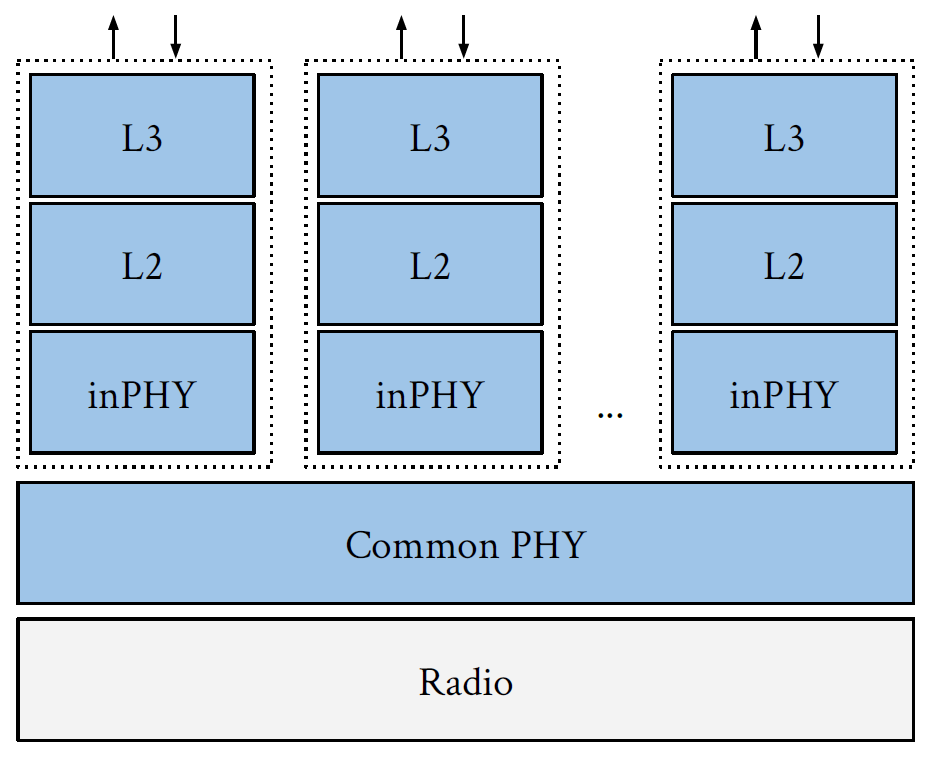
\includegraphics[width=0.7\textwidth]{figures/thesis_structure.png}
%\caption{thesis structure \citep{thesis_report}}
%\label{fig:thesis_structure}
%\end{figure}
%
%
%The system was made to prove if the method could work for a \gls{MTC} type of connection also. In this way they made a proof of concept product that emulated 15 devices using a 5 MHz bandwidth. They also proved that smaller bandwidth allowed the system to emulate more devices. The UEE used the the srsUE as a framework while the BSE used the \gls{OAI}. \citep{thesis_report} 
%
%The design of the \gls{MITE} relies heavily on the work done in this project. However as it is intended to use the \gls{NB-IoT} protocol instead of \gls{LTE} it is necessary to use another version of srsUE as well as another framework entirely for the \gls{BS} emulator. The \gls{BS} emulator will instead rely on the Amarisoft BSE.
%
%%\section{General Setup}
%\section{Basestation emulator}
%As found in the \autoref{ch:Introduction} there is two possibilities when choosing the \gls{BSE}, Amairsoft and SRS. It has been chosen to work with the Amarisoft \gls{BSE}, as it provides the necessary features and comes with support. The SRS \gls{BSE} is not yet fully developed so it might require a lot more time to get working. Another alternative altogether is the Keysight E7515A UXM, it also provides the needed features it is just a lot more expensive. Therefore the \gls{BSE} chosen is the Amarisoft LTE 100.
%
%Amarisoft LTE 100 features LTE, LTE-A, LTE-M and NB-IoT protocols.    For the NB-IoT protocol it specifically features\citep{Amarisoft_solutions}:
%
%\begin{itemize}
%\item NB-IoT release 14 compliant
%\item Single-tone and multi-tone category NB1 and NB2 UE support
%\item 15 kHz and 3.75 kHz subcarrier spacing are supported
%\item All operation modes (in-band, guard band and standalone) are supported
%\item Multiple NB-IoT and LTE cells can be used at the same time in the same eNodeB
%\item Support of multiple coverage levels
%\item Support of all NPDCCH, NPDSCH, NPUSCH and NPRACH configurations
%\item Support of control plane CIoT optimization
%\item Support of multi-DRB mode
%\end{itemize}
%
%\section{User Equipment Emulator}
%\subsection{Quectel}
%\subsection{SRS UE}
%
%
% and the channel emulator will be implemented only as a simple \gls{PL} factor. 



\chapter{Performance Evaluation}
%Here should be an introduction of what we will test (the emulator and/or the protocol). 

To evaluate the designed system a few key parameters are set as main pointers. This include the amount of users and the configurability of the solution, as well as it physical limitations. The system is then used to test the NB-IoT protocol, to show the usability of the solution. Some of these evaluation points have been described prior but a complete list is provided in the following section.

\section{Evaluation Points}
%Here should be a list of all requirement that is tested and criteria for passed not passed. 
The key parameters can be spilt into two groups: the emulator and the protocol. These groups are independent of each other in the sense that any other emulator should reveal the same results for the same protocol, given the same parameters.

\begin{itemize}
\item Emulator
	\begin{enumerate}
	\item Amount of users %(CPU,RAM) 
		\begin{itemize}
		\item Support TBD active users and TBD users total
		\end{itemize}
	\item Configurability  %(Channel, Number of UEs, etc.)
		\begin{itemize}
		\item Changeable parameters: Channel type, path loss, number of devices, data profile
		\end{itemize}
	\item Limits 
		\begin{itemize}
		\item Should support a output power up to 23 dB with a range of TBD dB
		\item Should support the frequency range from TBD to TBD and a bandwith up to TBD
		\end{itemize}
	\end{enumerate}
\item Protocol
	\begin{enumerate}[resume]
	\item  Ultra-low Complexity Devices
		\begin{itemize}
		\item The \gls{UE} has a sample rate of 240 KHz
		\item Only supports \gls{TBCC}
		\item Half-duplex
		\item Uses \gls{SISO} connection
		\end{itemize}
	\item Improved Coverage
		\begin{itemize}
		\item Support a \gls{MCL} of 164 dB
		\item Improve coverage by introducing \gls{CE} levels 
		\end{itemize}
	\item Support Massive Number of Devices 
		\begin{itemize}
		\item Support 52547 devices per cell-site sector based on a TBD data profile
		\end{itemize}
	\item Improved Power Efficiency
		\begin{itemize}
		\item  Achieve a battery life time of 10 years with a battery capacity of 5 Wh
		\item Using \gls{CE} to minimize Power amplifier backoff increasing efficiency
		\item Utilize \gls{cDRX}, \gls{eDRX} and \gls{PSM} to increase efficiency
	\end{itemize}
	\item Deployment flexibility
		\begin{itemize}
		\item The system should be able to be deployed inside legacy \gls{LTE}.
		\item The system should be able to be deployed as a stand alone solution.
		\end{itemize}
	\end{enumerate}
\end{itemize}
%\item Massiveness
%	\begin{enumerate}
%	\item Time to connect vs. connection request per second 
%	\item Data rate vs. number of users
%	\item Spectrum use vs. number of users
%	\item Interference level vs. number of users
%	\end{enumerate}
%\item Power
%	\begin{enumerate}
%	\item Energy consumption for attach.
%	\item Energy consumption vs. data rate
%	\item Energy consumption vs. coverage level
%	\item Energy consumption vs. operation mode
%	\item Energy consumption vs. number of UEs
%	\item Energy consumption vs. UE state (Connected (cDRX), eDRX, PSM, Off)
%	\end{enumerate}
%\end{enumerate}


Based on both the focus explained in \autoref{ch:Introduction} as well as some issues with the emulator explained TBD. The only points that is actually tested are: \todo{check if this is correct later}

\begin{itemize}
\item Emulator
	\begin{enumerate}
	\item[1.] Amount of users %(CPU,RAM) 
	\item[2.] Configurability %(Channel, Number of UEs, etc.)
%	\item[3.] Power control 
	\end{enumerate}
\item Protocol
	\begin{enumerate}
%	\item[4.] Ultra-low Complexity Devices
%	\item[5.] Improved Coverage
	\item[6.] Support Massive Number of Devices 
	\item[7.] Improved Power Efficiency
	\item[8.] Deployment flexibility
	\end{enumerate}
\end{itemize}

\newpage

\section{General Test Setup}
%Here should be a description of the general setup (including figure) used in all test and a list of baseline values for all parameters. Including physical setup, BSE, UEE.

The general way to setup the emulator is described here, some deviations occurs depending on the actual use of the system. A full setup is only needed when an external device is tested under the influence of a large number of interfering devices. The full setup can be seen in \autoref{fig:General_test_setup}.

\begin{figure}[H]
\centering
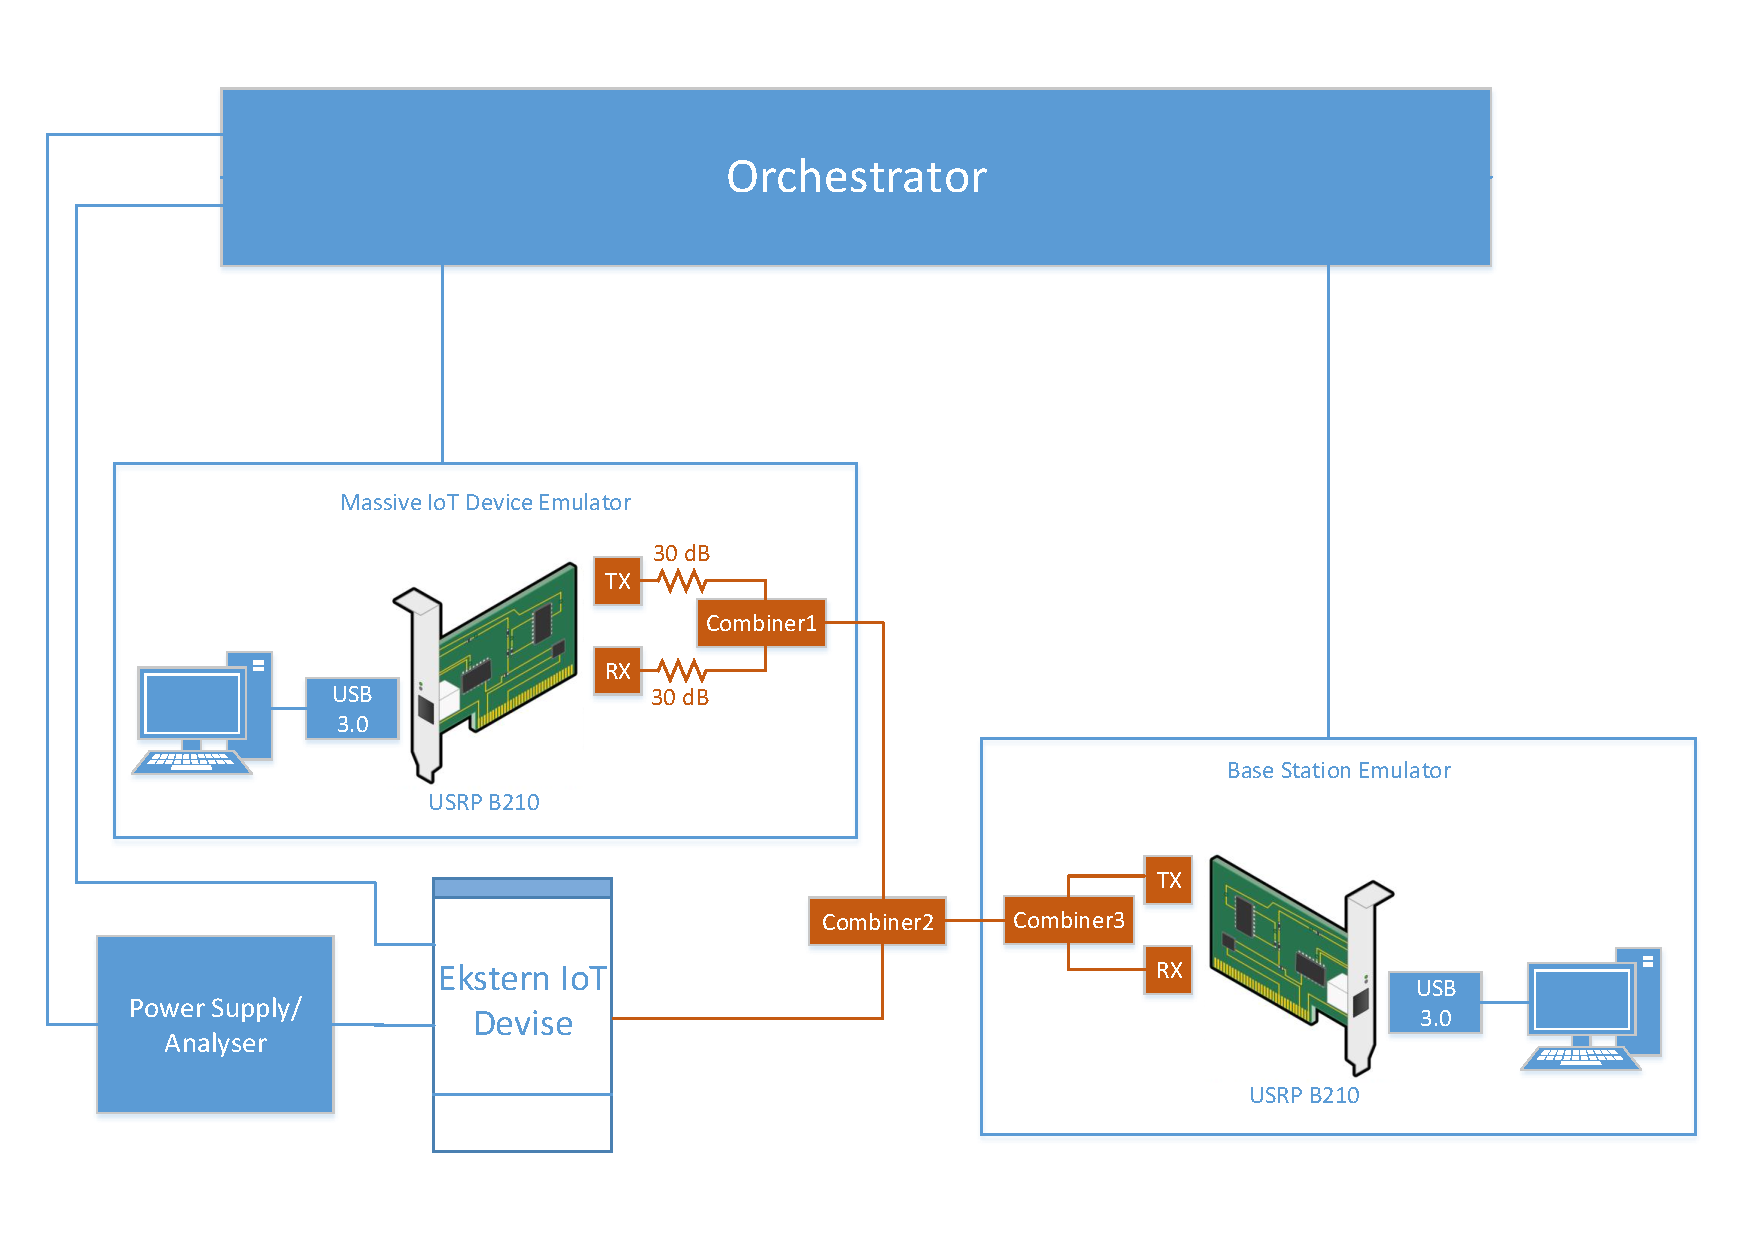
\includegraphics[width=\textwidth]{figures/General_test_setup.pdf}
\caption{General test setup, blue lines are control connections, orange lines are RF connections.}
\label{fig:General_test_setup}
\end{figure}

As seen in \autoref{fig:General_test_setup}, a \gls{TAP} orchestrator maintain the system. The orchestrator has a \gls{LAN} connection with each of the other elements with the exception of the external IoT device which is dependent on the device but typically is a serial connection. The \gls{PSU}s connection with the external IoT device is plain wires used to power on and analyse the power consumption of the device. Both the massive IoT device emulator as well as the external IoT device is connected to a combiner using RF SMA cables, this combiner is connected to the \gls{BSE} also using a RF SMA cable. 

The massive IoT device emulator PC is connected using USB 3.0 to the USRP B210. Mounted on the TX1 and RX1 port is a 30 dB attenuator which is connected to a combiner using RF SMA cables the output of the combiner acts as the output of the emulator.

The \gls{BSE} is interchangeable if the UXM is used TxRx1/Rx1 on RF Transceiver A is used as input. If the Amarisoft BSE is used the input is a combiner connected to the TX1 and RX1 ports on a USRP B210 using RF SMA cables, which is connected to the PC using a USB 3.0 connector.

The initial settings of each component in the system can be seen in \autoref{tab:setup_parameters}.

\begin{table}[H]
\captionsetup{belowskip=0em}
\noindent
\centering
%\resizebox{!}{0.5\textheight}{
\begin{minipage}[t]{0.48\textwidth}
\begin{tabular}{|p{4cm}|p{2cm}|}
\hline
\multicolumn{2}{|c|}{\textbf{Power Supply/Analyser}}                         \\ \hline
Enable             & Off            \\ \hline
Volt               & 3.6 V          \\ \hline
Ampere             & 2.5 A          \\ \hline
Sample interval	   & 100 $\mu$s		\\ \hline
\multicolumn{2}{c}{}\\ \hline
\multicolumn{2}{|c|}{\textbf{Massive IoT Emulator}}                          \\ \hline
\textbf{Parameter} & \textbf{Value} \\ \hline
Number of devices  & 0              \\ \hline
Rx gain            & 40 dB          \\ \hline
Tx gain            & 40 dB          \\ \hline
R14                & False          \\ \hline
Dl\_EARFCN         & 6240           \\ \hline
UE\_category       & Nb1            \\ \hline
\end{tabular}
%\caption{Initial values of the parameters in the emulator.}
\end{minipage}% 
\hfill
\begin{minipage}[t]{0.48\textwidth}
\begin{tabular}{|p{4cm}|p{2cm}|}
\hline
\multicolumn{2}{|c|}{\textbf{Ekstern IoT device}}                            \\ \hline
Enable             & Off            \\ \hline
Dl\_EARFCN         & 6240           \\ \hline
\multicolumn{2}{c}{}\\ \hline
\multicolumn{2}{|c|}{\textbf{Base Station Emulator}}                         \\ \hline
Cell type          & NB-IoT         \\ \hline
Number of cells    & 1              \\ \hline
Operation mode     & Standalone     \\ \hline
Dl\_EARFCN         & 6240           \\ \hline
Cell ID            & 0              \\ \hline
Tx gain            & 89 dB          \\ \hline
R14                & False          \\ \hline
nprach\_detect\_ threshold  & 19 dB  \\ \hline
\end{tabular}
%\caption{Initial values of the parameters in the emulator.}
%\label{tab:setup_parameters}
\end{minipage}
\caption{Initial values of the parameters in the emulator.}
\label{tab:setup_parameters}
\end{table}


\section{Evaluation}
%Here should be a step by step procedure of all test for all requirements, maybe put tapplans in appendix.

%\subsection{Amount of Devices}

\subsection{Configurability}

%\subsection{Power Control}

%\subsection{Ultra-low Complexity Devices}

%\subsection{Improved Coverage}

%\subsection{Support Massive Number of Devices}

\subsection{Improved Power Efficiency}
\subsubsection{Test Overview}
From \appref{app:bat_model} it can be seen that to estimate the battery life time of a device the following parameters is needed.
\begin{itemize}
%\item $P_{device}$
%\item $E_{modem,on}$
\item $E_{sync}$
\item $E_{attach}$
\item $P_{tx}$
\item $P_{eDRX}$
\item $P_{PSM}$
\end{itemize}

However in a \gls{NB-IoT} system a multitude of parameters have an influence either in regards to the time it takes to transmit anything or in the energy consumed during a transmission, this is the case for all states and transitions the device experience. To account for all of this is to humongous a task for this project, therefore a couple of parameters is chosen to simplify this task. The downside of this is the reliability of the results as these can only be assume valid in cases where the other parameters are chosen to the same values as used in this project. The values chosen are CP format, operation mode, frequency and $P_{TX}$. The CP format and operation mode is chosen as these are some often mentioned parameters which also only has a few values, repetition could also be considered here however as four different channels can be repeated with each having its own specifying parameter it is chosen to set all repetition to 1 and leave this parameter up to further analysis. The frequency typically has a high influence on the hardware used it is therefore considered as well as the $P_{TX}$  

With these informations the only thing needed is the data profile, the same models are used here as in \citep{Power_article}. Model 1 transmit every hour and Model 2 transmit every 24 hours, transmission size is 100 bytes for both models. %\todo{see if standards have some specified data profiles.}

From a measurement perspective some of these parameters can and should be measured together, these are $E_{sync}$ and $E_{attach}$. This is because these steps are depending on each other and can not be separated for the measurements only in the post processing. These are collectively referred to as $E_{conn}$ or energy to connect the device to the cell. 

To test these parameters the following setup is modified from \autoref{fig:General_test_setup} to the following:

\begin{figure}[H]
\centering
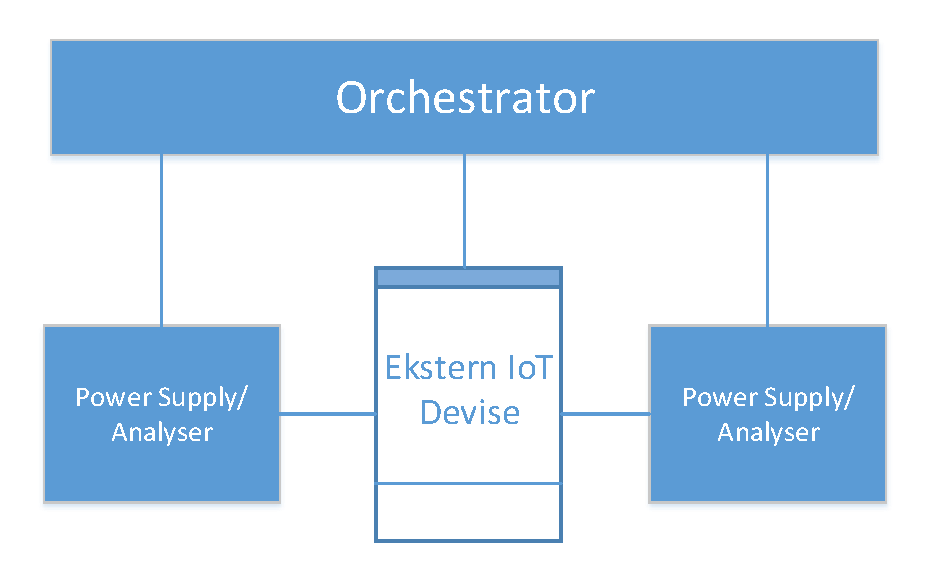
\includegraphics[width=0.5\textwidth]{figures/IPE_test_setup.pdf}
\caption{Setup used to test for the power efficiency of the \gls{DUT}'s}
\label{fig:IPE_test_setup}
\end{figure}

It should be noted that the \gls{DUT}'s in question have to power inputs, one for the device power and one for the RF modem power. Typically only the modem is connected to the power analyser. With the exception of measuring the device power where the the device power input is connected to the power analyser.

As the UXM is used as \gls{BSE} instead of Amarisoft the initial settings for this can be seen in \autoref{tab:UXM_initial_values}.

\begin{table}[H]
\centering
\begin{tabular}{|c|c|} \hline
\multicolumn{2}{|c|}{\textbf{UXM \gls{BSE}}} \\ \hline
Cell type			 & NB-IoT         \\ \hline
Number of cells		 & 1              \\ \hline
Operation mode		 & Standalone     \\ \hline
Host cell Dl\_EARFCN & 6240           \\ \hline
PRB offset			 & 0	          \\ \hline
Cell ID				 & 0              \\ \hline
Tx power			 & -80 dB/per 15 kHz \\ \hline
Repetition NPDSCH	 & 1	          \\ \hline
Max Repetition NPDCCH & 4	          \\ \hline
Repetition NPUSCH	 & 1	          \\ \hline
Repetition NPRACH	 & 1	          \\ \hline
CP format			 & Normal         \\ \hline
$P_{TX}$				 & 23 dBm         \\ \hline
MAC padding DL		 & off       	  \\ \hline
MAC padding UL		 & off       	  \\ \hline
\end{tabular}
\caption{Initial parameters of the UXM}
\label{tab:UXM_initial_values}
\end{table}

%\subsubsection{Device Power Consumption}
%
%To measure the device power, the power input to the device is used in the setup. The test is performed using the following procedure:
%
%\textbf{Test Procedure}
%\vspace{-1.5em}
%\begin{enumerate}
%\item Setup the \gls{DUT} as shown on \autoref{fig:IPE_test_setup}
%\item Put in settings as described in \autoref{tab:setup_parameters} and \autoref{tab:UXM_initial_values} 
%\item Turn on power supply 
%\item Measure power output over 2 min
%\item Save measurements as "<device>\_Power\_consumption"
%\item Turn off power supply
%\item Change to next \gls{DUT}
%\item Repeat step 1-7 for all \gls{DUT}s.
%\end{enumerate}
%
%\textbf{Results}\\
%\begin{table}[H]
%\centering
%\begin{tabular}{|c|c|c|c|}\hline
%\textbf{Device}	& Quectel	& Telit & Ublox \\ \hline
%$\mathbf{P_{device}}$	& & & \\ \hline
%\end{tabular}
%\caption{Average power consumption of the \gls{DUT}s}
%\label{tab:device_power_results}
%\end{table}

\subsubsection{Energy to Connect the Device to the Cell}

To measure the energy used to connect the device to the cell the following procedure is used.

\textbf{Test Procedure}\\
\begin{enumerate}
\item Setup the \gls{DUT} as shown on \autoref{fig:IPE_test_setup}
\item Turn on power supply 
\item Input settings as described in \autoref{tab:UXM_initial_values}
\item Input chosen value of chosen parameter
\item Put device in disconnected state 
\item Input to log "start <Parameters used> <Parameter value>"
\item Turn on power analyser
\item Verify connection to cell
\item Release DUT
\item Turn off power analyser
\item Save L3 log from UXM as "Attach\_<Parameters used>\_<Parameters value>.xml"
\item Turn off power supply
\item Change to next value
\item Repeat step 4-13 for all values
\item Save measurements as "Attach\_<Parameters used>\_MessageLog.csv"
\item Change to next parameter
\item Repeat step 3-16 for all parameters
\end{enumerate}


\textbf{Results}\\
\begin{figure}[H]
\centering
\begin{minipage}[tbp]{0.58\textwidth}
\resizebox{\textwidth}{!}{
% This file was created by matlab2tikz.
%
%The latest updates can be retrieved from
%  http://www.mathworks.com/matlabcentral/fileexchange/22022-matlab2tikz-matlab2tikz
%where you can also make suggestions and rate matlab2tikz.
%
\definecolor{mycolor1}{rgb}{0.00000,0.44700,0.74100}%
%
\begin{tikzpicture}
\begin{axis}[%
width=\textwidth,
height=0.66\textwidth,
at={(0.758in,0.481in)},
scale only axis,
xmin=0,
xmax=16,
xlabel={Time [s]},
ymin=-0.1,
ymax=0.8,
ylabel={Power Consumption [W]},
axis background/.style={fill=white}
]
\addplot [color=mycolor1,only marks,mark=*,mark options={solid},forget plot]
  table[row sep=crcr]{%
0	-0.00027465822\\
0.007168	-0.000137329092\\
0.014336	0\\
0.021504	-0.000137329092\\
0.028672	-0.000320435136\\
0.03584	-0.000160217568\\
0.043008	-0.000137329092\\
0.050176	-0.000137329092\\
0.057344	-4.5776088e-05\\
0.064512	-9.1553004e-05\\
0.07168	0.000205992828\\
0.078848	-0.00036621108\\
0.086016	-0.00027465822\\
0.093184	-0.000183106044\\
0.100352	-0.000251770572\\
0.10752	-0.00041198724\\
0.114688	-0.00057220488\\
0.121856	-0.000228882132\\
0.129024	-0.00041198724\\
0.136192	-4.5776088e-05\\
0.14336	4.5776088e-05\\
0.150528	-0.00059509332\\
0.157696	-0.00054931644\\
0.164864	-0.0006637572\\
0.172032	-0.000228882132\\
0.1792	-0.000114440652\\
0.186368	0.00034332192\\
0.193536	-0.000320435136\\
0.200704	-0.00018310518\\
0.207872	-4.5776916e-05\\
0.21504	-0.000183106044\\
0.222208	-0.00057220488\\
0.229376	0.000251769744\\
0.236544	-0.00048065184\\
0.243712	6.8664564e-05\\
0.25088	-0.00052642872\\
0.258048	-0.000228882132\\
0.265216	-2.28884616e-05\\
0.272384	-0.00043487568\\
0.279552	-0.000160217568\\
0.28672	-0.0004577634\\
0.293888	0.00018310518\\
0.301056	-0.000160217568\\
0.308224	-0.00054931644\\
0.315392	-0.000160217568\\
0.32256	-0.000205993656\\
0.329728	-4.5776088e-05\\
0.336896	-0.000228882132\\
0.344064	-0.000114440652\\
0.351232	-0.000160217568\\
0.3584	-0.000160217568\\
0.365568	-0.00045776412\\
0.372736	-0.00036621108\\
0.379904	-0.00061798104\\
0.387072	-0.00070953408\\
0.39424	-0.00043487568\\
0.401408	-9.1553004e-05\\
0.408576	-0.00027465822\\
0.415744	0\\
0.422912	-0.000160217568\\
0.43008	-0.000251769744\\
0.437248	-0.00057220488\\
0.444416	-0.00041198724\\
0.451584	-0.000160217568\\
0.458752	-0.000183106044\\
0.46592	-6.8664564e-05\\
0.473088	4.5776088e-05\\
0.480256	-0.000251769744\\
0.487424	0.0003890988\\
0.494592	-0.00018310518\\
0.50176	-0.000320434308\\
0.508928	2.28876264e-05\\
0.516096	-0.00043487568\\
0.523264	-0.00041198724\\
0.530432	-9.1553004e-05\\
0.5376	0.00016021674\\
0.544768	-0.00018310518\\
0.551936	-0.00029754666\\
0.559104	-0.0006637572\\
0.566272	0\\
0.57344	0.000114440652\\
0.580608	-0.000160217568\\
0.587776	-0.000160217568\\
0.594944	-0.0006637572\\
0.602112	-0.000183106044\\
0.60928	-0.00057220488\\
0.616448	-0.000137329092\\
0.623616	-0.000526428\\
0.630784	0.00018310518\\
0.637952	-6.8664564e-05\\
0.64512	9.1552176e-05\\
0.652288	0\\
0.659456	2.28876264e-05\\
0.666624	-0.000251770572\\
0.673792	-0.000343322748\\
0.68096	-0.0006637572\\
0.688128	-0.000160217568\\
0.695296	-0.000228882132\\
0.702464	0\\
0.709632	-0.0004577634\\
0.7168	-0.00029754666\\
0.723968	0.000114440652\\
0.731136	-0.0004577634\\
0.738304	-0.000343322748\\
0.745472	-0.000137329092\\
0.75264	4.5776088e-05\\
0.759808	0.000205993656\\
0.766976	-0.000343322748\\
0.774144	-0.000343322748\\
0.781312	4.5776088e-05\\
0.78848	-0.00029754666\\
0.795648	-0.00027465822\\
0.802816	4.5776088e-05\\
0.809984	-0.00041198724\\
0.817152	-9.1553004e-05\\
0.82432	2.28876264e-05\\
0.831488	-0.000228882132\\
0.838656	-0.0003890988\\
0.845824	-2.28884616e-05\\
0.852992	-0.000228882132\\
0.86016	-4.5776916e-05\\
0.867328	-0.000160217568\\
0.874496	-0.0004577634\\
0.881664	-0.000137329092\\
0.888832	-0.00029754666\\
0.896	0.00016021674\\
0.903168	-0.000343322748\\
0.910336	-0.0005950926\\
0.917504	-0.00027465822\\
0.924672	-0.00057220488\\
0.93184	-0.000114440652\\
0.939008	-4.5776916e-05\\
0.946176	9.1552176e-05\\
0.953344	0\\
0.960512	6.8664564e-05\\
0.96768	6.86637e-05\\
0.974848	-0.000160217568\\
0.982016	-4.5776088e-05\\
0.989184	-0.00054931644\\
0.996352	-0.00011444148\\
1.00352	-0.00050354028\\
1.010688	-0.000526428\\
1.017856	0.000137329092\\
1.025024	-0.000205993656\\
1.032192	0\\
1.03936	-0.00029754666\\
1.046528	-0.0005950926\\
1.053696	-0.00061798104\\
1.060864	-0.000205993656\\
1.068032	-0.000160217568\\
1.0752	-0.00011444148\\
1.082368	-0.000297545832\\
1.089536	-0.000343322748\\
1.096704	-0.0003890988\\
1.103872	-0.0003890988\\
1.11104	-0.00068664564\\
1.118208	0.00018310518\\
1.125376	0\\
1.132544	6.8664564e-05\\
1.139712	6.86637e-05\\
1.14688	-0.00036621108\\
1.154048	-0.00054931644\\
1.161216	-0.000343322748\\
1.168384	-0.000137329092\\
1.175552	-0.000228882132\\
1.18272	-0.00054931644\\
1.189888	-0.00068664564\\
1.197056	-0.00011444148\\
1.204224	-6.8664564e-05\\
1.211392	-0.00036621108\\
1.21856	-0.000343322748\\
1.225728	-0.00011444148\\
1.232896	-0.00018310518\\
1.240064	-0.000320435136\\
1.247232	-0.00027465822\\
1.2544	-0.000320434308\\
1.261568	0\\
1.268736	-0.000251770572\\
1.275904	-0.00027465822\\
1.283072	-0.00061798104\\
1.29024	0.0138244608\\
1.297408	0.0141448968\\
1.304576	0.0188598636\\
1.311744	0.0189056376\\
1.318912	0.023666382\\
1.32608	0.01966095\\
1.333248	0.0197753904\\
1.340416	0.104026788\\
1.347584	0.102653496\\
1.354752	0.102745044\\
1.36192	0.103019724\\
1.369088	0.102127068\\
1.376256	0.101989728\\
1.383424	0.103042584\\
1.390592	0.101966868\\
1.39776	0.101989728\\
1.404928	0.102287304\\
1.412096	0.104209884\\
1.419264	0.103248576\\
1.426432	0.103820796\\
1.4336	0.103729248\\
1.440768	0.104026788\\
1.447936	0.1036377\\
1.455104	0.103294368\\
1.462272	0.104301468\\
1.46944	0.105857856\\
1.476608	0.108352656\\
1.483776	0.105789168\\
1.490944	0.106361388\\
1.498112	0.105880752\\
1.50528	0.10583496\\
1.512448	0.106155396\\
1.519616	0.106979364\\
1.526784	0.10949706\\
1.533952	0.111213684\\
1.54112	0.108489996\\
1.548288	0.109909044\\
1.555456	0.110389716\\
1.562624	0.112197888\\
1.569792	0.11592864\\
1.57696	0.112907412\\
1.584128	0.11357118\\
1.591296	0.1131363\\
1.598464	0.11286162\\
1.605632	0.112472532\\
1.6128	0.115219116\\
1.619968	0.115173324\\
1.627136	0.114784236\\
1.634304	0.116249076\\
1.641472	0.116134632\\
1.64864	0.116455068\\
1.655808	0.11606598\\
1.662976	0.116546616\\
1.670144	0.118583676\\
1.677312	0.119773872\\
1.68448	0.119178756\\
1.691648	0.120826728\\
1.698816	0.12119292\\
1.705984	0.123046884\\
1.713152	0.123847956\\
1.72032	0.123870852\\
1.727488	0.124900812\\
1.734656	0.126319896\\
1.741824	0.12718962\\
1.748992	0.128585808\\
1.75616	0.128036484\\
1.763328	0.127967832\\
1.770496	0.128585808\\
1.777664	0.145133964\\
1.784832	0.1537857\\
1.792	0.153579708\\
1.799168	0.153396612\\
1.806336	0.1537857\\
1.813504	0.153099072\\
1.820672	0.15319062\\
1.82784	0.153396612\\
1.835008	0.151496892\\
1.842176	0.153327924\\
1.849344	0.0260238636\\
1.856512	0.0298919664\\
1.86368	0.0287704476\\
1.870848	0.0258865344\\
1.878016	0.028930662\\
1.885184	0.036781308\\
1.892352	0.0302352876\\
1.89952	0.037033092\\
1.906688	0.036186228\\
1.913856	0.0296630856\\
1.921024	0.0331649784\\
1.928192	0.042068484\\
1.93536	0.047904984\\
1.942528	0.0323638884\\
1.949696	0.037078848\\
1.956864	0.076766976\\
1.964032	0.0332336412\\
1.9712	0.039550788\\
1.978368	0.043601976\\
1.985536	0.03609468\\
1.992704	0.03588867\\
1.999872	0.0334854108\\
2.00704	0.0326614356\\
2.014208	0.03872682\\
2.021376	0.0359573364\\
2.028544	0.03362274\\
2.035712	0.044036856\\
2.04288	0.0303955056\\
2.050048	0.0336456288\\
2.057216	0.0338745096\\
2.064384	0.0335540772\\
2.071552	0.043395984\\
2.07872	0.038795472\\
2.085888	0.03362274\\
2.093056	0.036483768\\
2.100224	0.030830382\\
2.107392	0.0330047604\\
2.11456	0.0351333612\\
2.121728	0.0334396368\\
2.128896	0.0325927728\\
2.136064	0.034103394\\
2.143232	0.0331420896\\
2.1504	0.03552246\\
2.157568	0.0335998512\\
2.164736	0.0337371804\\
2.171904	0.0333938592\\
2.179072	0.03325653\\
2.18624	0.0359802252\\
2.193408	0.033782958\\
2.200576	0.0332336412\\
2.207744	0.0330505344\\
2.214912	0.033576966\\
2.22208	0.03588867\\
2.229248	0.0330505344\\
2.236416	0.033576966\\
2.243584	0.0338745096\\
2.250752	0.041152968\\
2.25792	0.0339660648\\
2.265088	0.051269544\\
2.272256	0.044403084\\
2.279424	0.031402584\\
2.286592	0.038314836\\
2.29376	0.0336456288\\
2.300928	0.038658132\\
2.308096	0.03918456\\
2.315264	0.0352706904\\
2.322432	0.0335082996\\
2.3296	0.0336685176\\
2.336768	0.042137136\\
2.343936	0.0346755996\\
2.351104	0.042503364\\
2.358272	0.038818368\\
2.36544	0.0344238264\\
2.372608	0.0319290156\\
2.379776	0.037147536\\
2.386944	0.0300292956\\
2.394112	0.0344924892\\
2.40128	0.0334396368\\
2.408448	0.0336456288\\
2.415616	0.0326614356\\
2.422784	0.0337142952\\
2.429952	0.0308761596\\
2.43712	0.03289032\\
2.444288	0.039367656\\
2.451456	0.03325653\\
2.458624	0.0337142952\\
2.465792	0.03362274\\
2.47296	0.048568716\\
2.480128	0.0314712504\\
2.487296	0.044471736\\
2.494464	0.0350189208\\
2.501632	0.036506664\\
2.5088	0.0321578964\\
2.515968	0.0257949828\\
2.523136	0.0204162588\\
2.530304	0.0205306992\\
2.537472	0.020553588\\
2.54464	0.0205078104\\
2.551808	0.0208053576\\
2.558976	0.0205306992\\
2.566144	0.0203704812\\
2.573312	0.0203247072\\
2.58048	0.02039337\\
2.587648	0.0206222508\\
2.594816	0.020553588\\
2.601984	0.020874024\\
2.609152	0.0201187116\\
2.61632	0.020553588\\
2.623488	0.0205078104\\
2.630656	0.0204162588\\
2.637824	0.0205306992\\
2.644992	0.0205764768\\
2.65216	0.0207366948\\
2.659328	0.0204162588\\
2.666496	0.0201644892\\
2.673664	0.0207366948\\
2.680832	0.0208511352\\
2.688	0.0205764768\\
2.695168	0.0206909172\\
2.702336	0.02039337\\
2.709504	0.020874024\\
2.716672	0.0205306992\\
2.72384	0.0202789296\\
2.731008	0.0207824688\\
2.738176	0.0205306992\\
2.745344	0.0209426868\\
2.752512	0.0203704812\\
2.75968	0.0204620364\\
2.766848	0.020347596\\
2.774016	0.020874024\\
2.781184	0.0204620364\\
2.788352	0.0246505752\\
2.79552	0.02039337\\
2.802688	0.0204620364\\
2.809856	0.0210113532\\
2.817024	0.020187378\\
2.824192	0.0206680284\\
2.83136	0.0205993656\\
2.838528	0.020553588\\
2.845696	0.0203018184\\
2.852864	0.0205993656\\
2.860032	0.0206222544\\
2.8672	0.020713806\\
2.874368	0.0203475924\\
2.881536	0.0208053576\\
2.888704	0.0203247072\\
2.895872	0.0201644892\\
2.90304	0.0205764768\\
2.910208	0.0208282464\\
2.917376	0.0208053576\\
2.924544	0.0207595836\\
2.931712	0.0205078104\\
2.93888	0.0204162588\\
2.946048	0.020553588\\
2.953216	0.0204620364\\
2.960384	0.0206222508\\
2.967552	0.0205306992\\
2.97472	0.0205993656\\
2.981888	0.0204620364\\
2.989056	0.0207366948\\
2.996224	0.020347596\\
3.003392	0.0204849252\\
3.01056	0.0204162588\\
3.017728	0.0203475924\\
3.024896	0.0203018184\\
3.032064	0.0202560408\\
3.039232	0.0204620364\\
3.0464	0.020713806\\
3.053568	0.0204162588\\
3.060736	0.0203018184\\
3.067904	0.0208969128\\
3.075072	0.020553588\\
3.08224	0.0205306992\\
3.089408	0.0204849252\\
3.096576	0.02039337\\
3.103744	0.0204162588\\
3.110912	0.0201416004\\
3.11808	0.0206909172\\
3.125248	0.0205764768\\
3.132416	0.0203247072\\
3.139584	0.020347596\\
3.146752	0.0207595836\\
3.15392	0.0200500488\\
3.161088	0.020713806\\
3.168256	0.0200042712\\
3.175424	0.0203247072\\
3.182592	0.0205764768\\
3.18976	0.0202560408\\
3.196928	0.020713806\\
3.204096	0.0208053576\\
3.211264	0.020187378\\
3.218432	0.0204391476\\
3.2256	0.0205306992\\
3.232768	0.02039337\\
3.239936	0.0203247072\\
3.247104	0.0207366948\\
3.254272	0.020713806\\
3.26144	0.020553588\\
3.268608	0.0203475924\\
3.275776	0.0203247072\\
3.282944	0.020072934\\
3.290112	0.0204849216\\
3.29728	0.0205993656\\
3.304448	0.0206451396\\
3.311616	0.0208053576\\
3.318784	0.024513246\\
3.325952	0.0209655756\\
3.33312	0.0205764768\\
3.340288	0.0202102632\\
3.347456	0.0200729376\\
3.354624	0.0202102668\\
3.361792	0.0203247072\\
3.36896	0.0202102668\\
3.376128	0.0206451396\\
3.383296	0.02002716\\
3.390464	0.0204620364\\
3.397632	0.0208282464\\
3.4048	0.0204391476\\
3.411968	0.020713806\\
3.419136	0.020233152\\
3.426304	0.0207595836\\
3.433472	0.0203704812\\
3.44064	0.0203704812\\
3.447808	0.0206909172\\
3.454976	0.0207824688\\
3.462144	0.020347596\\
3.469312	0.0204849252\\
3.47648	0.0205993656\\
3.483648	0.020553588\\
3.490816	0.0208053576\\
3.497984	0.0204162588\\
3.505152	0.0206680284\\
3.51232	0.0204162588\\
3.519488	0.0199584936\\
3.526656	0.0200729376\\
3.533824	0.0206222544\\
3.540992	0.02039337\\
3.54816	0.0205078104\\
3.555328	0.0204391476\\
3.562496	0.0204849216\\
3.569664	0.0209655756\\
3.576832	0.0204391476\\
3.584	0.0202789296\\
3.591168	0.020233152\\
3.598336	0.0204620364\\
3.605504	0.020874024\\
3.612672	0.020713806\\
3.61984	0.020713806\\
3.627008	0.0206909172\\
3.634176	0.0202789296\\
3.641344	0.0205306992\\
3.648512	0.0203018184\\
3.65568	0.0205306992\\
3.662848	0.0204391476\\
3.670016	0.0208511352\\
3.677184	0.0204620364\\
3.684352	0.0202789296\\
3.69152	0.0205993656\\
3.698688	0.0203475924\\
3.705856	0.0201187116\\
3.713024	0.0200729376\\
3.720192	0.0206680284\\
3.72736	0.0205764768\\
3.734528	0.0207824688\\
3.741696	0.020874024\\
3.748864	0.0204849216\\
3.756032	0.0201644892\\
3.7632	0.0202102668\\
3.770368	0.0208969128\\
3.777536	0.0204391476\\
3.784704	0.0200958228\\
3.791872	0.0199356084\\
3.79904	0.0204849252\\
3.806208	0.0232086168\\
3.813376	0.024513246\\
3.820544	0.0223388676\\
3.827712	0.020233152\\
3.83488	0.020553588\\
3.842048	0.0206222544\\
3.849216	0.0205306992\\
3.856384	0.02002716\\
3.863552	0.0206222544\\
3.87072	0.0202560408\\
3.877888	0.0202789296\\
3.885056	0.0205078104\\
3.892224	0.020187378\\
3.899392	0.0203018184\\
3.90656	0.0206451396\\
3.913728	0.02039337\\
3.920896	0.0202560408\\
3.928064	0.020919798\\
3.935232	0.0206222544\\
3.9424	0.0206909172\\
3.949568	0.0204620364\\
3.956736	0.0204162588\\
3.963904	0.020233152\\
3.971072	0.020553588\\
3.97824	0.0202560408\\
3.985408	0.0204391476\\
3.992576	0.0203247072\\
3.999744	0.0204391476\\
4.006912	0.020553588\\
4.01408	0.0207366948\\
4.021248	0.0205306992\\
4.028416	0.0204391476\\
4.035584	0.0203704812\\
4.042752	0.0203018184\\
4.04992	0.0201416004\\
4.057088	0.020713806\\
4.064256	0.020187378\\
4.071424	0.0204849216\\
4.078592	0.020187378\\
4.08576	0.0202102668\\
4.092928	0.0205764768\\
4.100096	0.0205993656\\
4.107264	0.0205764768\\
4.114432	0.0208053576\\
4.1216	0.0201416004\\
4.128768	0.0203247072\\
4.135936	0.0208282464\\
4.143104	0.0205993656\\
4.150272	0.0210571272\\
4.15744	0.0202102668\\
4.164608	0.0205306992\\
4.171776	0.0206909172\\
4.178944	0.0211715676\\
4.186112	0.020553588\\
4.19328	0.0206680284\\
4.200448	0.020553588\\
4.207616	0.0206680284\\
4.214784	0.020187378\\
4.221952	0.0204620364\\
4.22912	0.0197753904\\
4.236288	0.0206222544\\
4.243456	0.0205993656\\
4.250624	0.02039337\\
4.257792	0.0205764768\\
4.26496	0.0208511352\\
4.272128	0.0206222544\\
4.279296	0.02002716\\
4.286464	0.0207595836\\
4.293632	0.0204162588\\
4.3008	0.0206451396\\
4.307968	0.0205993656\\
4.315136	0.028244016\\
4.322304	0.200042712\\
4.329472	0.22570038\\
4.33664	0.243667584\\
4.343808	0.21283722\\
4.350976	0.254035944\\
4.358144	0.233001684\\
4.365312	0.245521512\\
4.37248	0.22190094\\
4.379648	0.253761264\\
4.386816	0.24895476\\
4.393984	0.246894804\\
4.401152	0.0249481188\\
4.40832	0.020553588\\
4.415488	0.149894712\\
4.422656	0.19953918\\
4.429824	0.232017516\\
4.436992	0.152389512\\
4.44416	0.14955138\\
4.451328	0.201919536\\
4.458496	0.155158992\\
4.465664	0.155754072\\
4.472832	0.200958264\\
4.48	0.19983672\\
4.487168	0.0242843616\\
4.494336	0.153282168\\
4.501504	0.201553344\\
4.508672	0.152458164\\
4.51584	0.159553512\\
4.523008	0.201095568\\
4.530176	0.197937\\
4.537344	0.151908876\\
4.544512	0.160995492\\
4.55168	0.201416004\\
4.558848	0.150627132\\
4.566016	0.0281753532\\
4.573184	0.153671256\\
4.580352	0.201782232\\
4.58752	0.155342088\\
4.594688	0.15319062\\
4.601856	0.200386044\\
4.609024	0.201347352\\
4.616192	0.15541074\\
4.62336	0.156967164\\
4.630528	0.201507552\\
4.637696	0.151062012\\
4.644864	0.0321807852\\
4.652032	0.0286331184\\
4.6592	0.0251998884\\
4.666368	0.0207366948\\
4.673536	0.0247421268\\
4.680704	0.020233152\\
4.687872	0.02039337\\
4.69504	0.024513246\\
4.702208	0.0201416004\\
4.709376	0.219451896\\
4.716544	0.024765012\\
4.723712	0.0205764768\\
4.73088	0.202812192\\
4.738048	0.0247879044\\
4.745216	0.0208969128\\
4.752384	0.0208053576\\
4.759552	0.0202789296\\
4.76672	0.0206680284\\
4.773888	0.02039337\\
4.781056	0.0206222544\\
4.788224	0.0207366948\\
4.795392	0.0206222508\\
4.80256	0.149734476\\
4.809728	0.149322492\\
4.816896	0.14984892\\
4.824064	0.153831456\\
4.831232	0.2372589\\
4.8384	0.028083798\\
4.845568	0.0246963492\\
4.852736	0.02419281\\
4.859904	0.0205306992\\
4.867072	0.0204849252\\
4.87424	0.0248336784\\
4.881408	0.0208511352\\
4.888576	0.020713806\\
4.895744	0.0246963492\\
4.902912	0.0204620364\\
4.91008	0.208671552\\
4.917248	0.0247421268\\
4.924416	0.020233152\\
4.931584	0.0205993656\\
4.938752	0.0211715676\\
4.94592	0.0205764768\\
4.953088	0.0205306992\\
4.960256	0.0203018184\\
4.967424	0.150489792\\
4.974592	0.15232086\\
4.98176	0.150260904\\
4.988928	0.150398244\\
4.996096	0.150306696\\
5.003264	0.150100704\\
5.010432	0.1502838\\
5.0176	0.150329592\\
5.024768	0.221717844\\
5.031936	0.150970464\\
5.039104	0.150489792\\
5.046272	0.151268004\\
5.05344	0.150352488\\
5.060608	0.151359552\\
5.067776	0.14998626\\
5.074944	0.151657092\\
5.082112	0.149528484\\
5.08928	0.151794432\\
5.096448	0.149734476\\
5.103616	0.15188598\\
5.110784	0.0278091432\\
5.117952	0.0489807\\
5.12512	0.153259272\\
5.132288	0.249572736\\
5.139456	0.0277862544\\
5.146624	0.0290222172\\
5.153792	0.0274429296\\
5.16096	0.0280609128\\
5.168128	0.024513246\\
5.175296	0.0252914436\\
5.182464	0.0249481188\\
5.189632	0.0333709704\\
5.1968	0.0303268428\\
5.203968	0.0296630856\\
5.211136	0.274566636\\
5.218304	0.246734604\\
5.225472	0.155136096\\
5.23264	0.221008284\\
5.239808	0.024879456\\
5.246976	0.0249023412\\
5.254144	0.207778932\\
5.261312	0.050148\\
5.26848	0.214508052\\
5.275648	0.213203448\\
5.282816	0.0295257564\\
5.289984	0.44702892\\
5.297152	0.4543992\\
5.30432	0.44274888\\
5.311488	0.4561614\\
5.318656	0.44068896\\
5.325824	0.151176456\\
5.332992	0.201942432\\
5.34016	0.250602696\\
5.347328	0.0230255136\\
5.354496	0.0205306992\\
5.361664	0.0205764768\\
5.368832	0.0204391476\\
5.376	0.131629932\\
5.383168	0.224876376\\
5.390336	0.0251312256\\
5.397504	0.219383244\\
5.404672	0.0239181516\\
5.41184	0.030670164\\
5.419008	0.71953596\\
5.426176	0.72981252\\
5.433344	0.254631024\\
5.440512	0.15158844\\
5.44768	0.218284596\\
5.454848	0.21416472\\
5.462016	0.216911304\\
5.469184	0.198188784\\
5.476352	0.0205078104\\
5.48352	0.0205306992\\
5.490688	0.0206222508\\
5.497856	0.020553588\\
5.505024	0.020553588\\
5.512192	0.203590404\\
5.51936	0.0284271228\\
5.526528	0.71548452\\
5.533696	0.73143756\\
5.540864	0.7099686\\
5.548032	0.72892008\\
5.5552	0.70976268\\
5.562368	0.73123164\\
5.569536	0.71083836\\
5.576704	0.72988128\\
5.583872	0.71276076\\
5.59104	0.0250167816\\
5.598208	0.254241936\\
5.605376	0.0242843616\\
5.612544	0.0203704812\\
5.619712	0.0208969128\\
5.62688	0.0204391476\\
5.634048	0.209701548\\
5.641216	0.215057376\\
5.648384	0.0272827152\\
5.655552	0.72972108\\
5.66272	0.7143174\\
5.669888	0.72569268\\
5.677056	0.709236\\
5.684224	0.72921744\\
5.691392	0.71058636\\
5.69856	0.72985824\\
5.705728	0.70925904\\
5.712896	0.72990432\\
5.720064	0.204917904\\
5.727232	0.0245819088\\
5.7344	0.0204391476\\
5.741568	0.0202789296\\
5.748736	0.020553588\\
5.755904	0.0202789296\\
5.763072	0.020347596\\
5.77024	0.0204849252\\
5.777408	0.205810524\\
5.784576	0.197364816\\
5.791744	0.208534248\\
5.798912	0.213386544\\
5.80608	0.0312652548\\
5.813248	0.72809604\\
5.820416	0.72649368\\
5.827584	0.0285873408\\
5.834752	0.218719476\\
5.84192	0.153579708\\
5.849088	0.16181946\\
5.856256	0.213203448\\
5.863424	0.249435396\\
5.870592	0.157241808\\
5.87776	0.039253248\\
5.884928	0.0331192008\\
5.892096	0.216224676\\
5.899264	0.258567804\\
5.906432	0.230712876\\
5.9136	0.265663152\\
5.920768	0.172828692\\
5.927936	0.21196746\\
5.935104	0.268157952\\
5.942272	0.224601732\\
5.94944	0.168914808\\
5.956608	0.21986388\\
5.963776	0.238609296\\
5.970944	0.17191314\\
5.978112	0.209976192\\
5.98528	0.0334854108\\
5.992448	0.041770944\\
5.999616	0.043533324\\
6.006784	0.043373124\\
6.013952	0.0349731432\\
6.02112	0.20670318\\
6.028288	0.235450728\\
6.035456	0.161132796\\
6.042624	0.237464892\\
6.049792	0.223205544\\
6.05696	0.235656756\\
6.064128	0.208557108\\
6.071296	0.231445296\\
6.078464	0.227508552\\
6.085632	0.150581376\\
6.0928	0.20100402\\
6.099968	0.225082404\\
6.107136	0.197410572\\
6.114304	0.0249481188\\
6.121472	0.02039337\\
6.12864	0.0207595836\\
6.135808	0.0204391476\\
6.142976	0.0201644892\\
6.150144	0.151130664\\
6.157312	0.244239804\\
6.16448	0.149574276\\
6.171648	0.210227976\\
6.178816	0.215835552\\
6.185984	0.185485824\\
6.193152	0.253417968\\
6.20032	0.207206712\\
6.207488	0.22279356\\
6.214656	0.249435396\\
6.221824	0.224853516\\
6.228992	0.202995288\\
6.23616	0.202926636\\
6.243328	0.024513246\\
6.250496	0.0206222544\\
6.257664	0.0208511352\\
6.264832	0.0202560408\\
6.272	0.131446836\\
6.279168	0.22583772\\
6.286336	0.202239972\\
6.293504	0.221946696\\
6.300672	0.150260904\\
6.30784	0.21956634\\
6.315008	0.204849252\\
6.322176	0.22000122\\
6.329344	0.20803068\\
6.336512	0.214210512\\
6.34368	0.211257936\\
6.350848	0.1501236\\
6.358016	0.213912972\\
6.365184	0.0280151352\\
6.372352	0.0207366948\\
6.37952	0.0204162588\\
6.386688	0.0204162588\\
6.393856	0.0203018184\\
6.401024	0.0207366948\\
6.408192	0.0245361312\\
6.41536	0.223457328\\
6.422528	0.200798028\\
6.429696	0.147811896\\
6.436864	0.20070648\\
6.444032	0.225791928\\
6.4512	0.195350652\\
6.458368	0.248085036\\
6.465536	0.150833124\\
6.472704	0.223022448\\
6.479872	0.202857948\\
6.48704	0.15042114\\
6.494208	0.206085204\\
6.501376	0.217620828\\
6.508544	0.207344052\\
6.515712	0.21372984\\
6.52288	0.0246505752\\
6.530048	0.149574276\\
6.537216	0.216247536\\
6.544384	0.249755868\\
6.551552	0.217918404\\
6.55872	0.206886276\\
6.565888	0.151542648\\
6.573056	0.205169688\\
6.580224	0.225494388\\
6.587392	0.2039337\\
6.59456	0.22586058\\
6.601728	0.201782232\\
6.608896	0.254104596\\
6.616064	0.192695616\\
6.623232	0.0247879044\\
6.6304	0.0204162588\\
6.637568	0.0204391476\\
6.644736	0.0203247072\\
6.651904	0.0206222544\\
6.659072	0.201187116\\
6.66624	0.219406104\\
6.673408	0.245841984\\
6.680576	0.148338324\\
6.687744	0.207115164\\
6.694912	0.215515116\\
6.70208	0.205078104\\
6.709248	0.229248036\\
6.716416	0.21503448\\
6.723584	0.229980456\\
6.730752	0.151496892\\
6.73792	0.207778932\\
6.745088	0.151542648\\
6.752256	0.02455902\\
6.759424	0.0204162588\\
6.766592	0.02039337\\
6.77376	0.0207366948\\
6.780928	0.0209884644\\
6.788096	0.201210012\\
6.795264	0.215309124\\
6.802432	0.2419281\\
6.8096	0.151863084\\
6.816768	0.225173952\\
6.823936	0.201667788\\
6.831104	0.196723944\\
6.838272	0.207412704\\
6.84544	0.149963364\\
6.852608	0.204574572\\
6.859776	0.217323288\\
6.866944	0.206932068\\
6.874112	0.195991524\\
6.88128	0.0306472752\\
6.888448	0.282531708\\
6.895616	0.0248107896\\
6.902784	0.0204162588\\
6.909952	0.02039337\\
6.91712	0.19397736\\
6.924288	0.0274200444\\
6.931456	0.20553588\\
6.938624	0.212745672\\
6.945792	0.0310134888\\
6.95296	0.46089936\\
6.960128	0.4420854\\
6.967296	0.4585878\\
6.974464	0.43782804\\
6.981632	0.027717588\\
6.9888	0.200775132\\
6.995968	0.177406308\\
7.003136	0.256919832\\
7.010304	0.0212860116\\
7.017472	0.0211486824\\
7.02464	0.0204849252\\
7.031808	0.0206451396\\
7.038976	0.0203704812\\
7.046144	0.0206451396\\
7.053312	0.221054076\\
7.06048	0.149322492\\
7.067648	0.0280151352\\
7.074816	0.72404496\\
7.081984	0.72248832\\
7.089152	0.72246564\\
7.09632	0.71784216\\
7.103488	0.72447984\\
7.110656	0.71514144\\
7.117824	0.72576144\\
7.124992	0.71040348\\
7.13216	0.72846216\\
7.139328	0.206382744\\
7.146496	0.226203912\\
7.153664	0.201644892\\
7.160832	0.0249710076\\
7.168	0.132179256\\
7.175168	0.226203912\\
7.182336	0.0253601064\\
7.189504	0.1476288\\
7.196672	0.212470992\\
7.20384	0.0308990484\\
7.211008	0.72843948\\
7.218176	0.73599228\\
7.225344	0.0274429296\\
7.232512	0.242546076\\
7.23968	0.213455196\\
7.246848	0.218124396\\
7.254016	0.216407772\\
7.261184	0.199310292\\
7.268352	0.0247879044\\
7.27552	0.0277404768\\
7.282688	0.0309677112\\
7.289856	0.029617308\\
7.297024	0.230781564\\
7.304192	0.215538012\\
7.31136	0.22952268\\
7.318528	0.239524848\\
7.325696	0.150695784\\
7.332864	0.201782232\\
7.340032	0.226181016\\
7.3472	0.202766436\\
7.354368	0.225425736\\
7.361536	0.200958264\\
7.368704	0.223869312\\
7.375872	0.214416504\\
7.38304	0.22235868\\
7.390208	0.065071116\\
7.397376	0.0250625628\\
7.404544	0.0207824688\\
7.411712	0.0207824688\\
7.41888	0.0207595836\\
7.426048	0.13286592\\
7.433216	0.213340752\\
7.440384	0.190452564\\
7.447552	0.215423568\\
7.45472	0.208328256\\
7.461888	0.218559276\\
7.469056	0.2062683\\
7.476224	0.221992488\\
7.483392	0.20436858\\
7.49056	0.151039116\\
7.497728	0.202880844\\
7.504896	0.21503448\\
7.512064	0.201965328\\
7.519232	0.200180052\\
7.5264	0.0208053576\\
7.533568	0.0211029048\\
7.540736	0.0208053576\\
7.547904	0.0206909172\\
7.555072	0.200683584\\
7.56224	0.237762432\\
7.569408	0.16197966\\
7.576576	0.218719476\\
7.583744	0.205879212\\
7.590912	0.149803164\\
7.59808	0.254013048\\
7.605248	0.149894712\\
7.612416	0.212860116\\
7.619584	0.230575572\\
7.626752	0.215583804\\
7.63392	0.208785996\\
7.641088	0.195510852\\
7.648256	0.0242614728\\
7.655424	0.0206909172\\
7.662592	0.0206222544\\
7.66976	0.0206222544\\
7.676928	0.0208282464\\
7.684096	0.0203704812\\
7.691264	0.0206909172\\
7.698432	0.24179076\\
7.7056	0.149528484\\
7.712768	0.22586058\\
7.719936	0.200546244\\
7.727104	0.199928268\\
7.734272	0.206886276\\
7.74144	0.22263336\\
7.748608	0.203155524\\
7.755776	0.147880548\\
7.762944	0.151336656\\
7.770112	0.149917608\\
7.77728	0.2170944\\
7.784448	0.149528484\\
7.791616	0.211326588\\
7.798784	0.0280838016\\
7.805952	0.0205993656\\
7.81312	0.194457996\\
7.820288	0.219612096\\
7.827456	0.207344052\\
7.834624	0.221214276\\
7.841792	0.205284132\\
7.84896	0.223297128\\
7.856128	0.191390976\\
7.863296	0.229591368\\
7.870464	0.149871816\\
7.877632	0.247032144\\
7.8848	0.149894712\\
7.891968	0.226272564\\
7.899136	0.194503788\\
7.906304	0.0242843616\\
7.913472	0.0205078104\\
7.92064	0.0208282464\\
7.927808	0.0203018184\\
7.934976	0.0203018184\\
7.942144	0.20086668\\
7.949312	0.218353284\\
7.95648	0.207984924\\
7.963648	0.233184816\\
7.970816	0.15174864\\
7.977984	0.21256254\\
7.985152	0.15204618\\
7.99232	0.211280832\\
7.999488	0.21839904\\
8.006656	0.207458496\\
8.013824	0.220573404\\
8.020992	0.186195384\\
8.02816	0.25069428\\
8.035328	0.0242843616\\
8.042496	0.020874024\\
8.049664	0.0206451396\\
8.056832	0.0206451396\\
8.064	0.0204620364\\
8.071168	0.200546244\\
8.078336	0.200431836\\
8.085504	0.150306696\\
8.092672	0.205787664\\
8.09984	0.254470824\\
8.107008	0.202514652\\
8.114176	0.235267632\\
8.121344	0.206291196\\
8.128512	0.238151556\\
8.13568	0.148704516\\
8.142848	0.214988724\\
8.150016	0.151863084\\
8.157184	0.215263368\\
8.164352	0.0243759168\\
8.17152	0.0206222544\\
8.178688	0.0205764768\\
8.185856	0.0203018184\\
8.193024	0.22263336\\
8.200192	0.207481392\\
8.20736	0.224166852\\
8.214528	0.2395935\\
8.221696	0.224807724\\
8.228864	0.207092268\\
8.236032	0.193290696\\
8.2432	0.203018184\\
8.250368	0.150810228\\
8.257536	0.201095568\\
8.264704	0.147399912\\
8.271872	0.201164256\\
8.27904	0.224327088\\
8.286208	0.0246734604\\
8.293376	0.020553588\\
8.300544	0.0205078104\\
8.307712	0.0198898308\\
8.31488	0.0201416004\\
8.322048	0.030464172\\
8.329216	0.27321624\\
8.336384	0.0249710076\\
8.343552	0.232154856\\
8.35072	0.149711616\\
8.357888	0.216911304\\
8.365056	0.149894712\\
8.372224	0.22162626\\
8.379392	0.250900272\\
8.38656	0.223571772\\
8.393728	0.203521716\\
8.400896	0.214485156\\
8.408064	0.149734476\\
8.415232	0.230758632\\
8.4224	0.201805128\\
8.429568	0.188644392\\
8.436736	0.195259104\\
8.443904	0.0249252336\\
8.451072	0.1932678\\
8.45824	0.235908504\\
8.465408	0.154975896\\
8.472576	0.21986388\\
8.479744	0.0273742668\\
8.486912	0.205261236\\
8.49408	0.44709768\\
8.501248	0.45444492\\
8.508416	0.44561016\\
8.515584	0.45256788\\
8.522752	0.216842652\\
8.52992	0.149963364\\
8.537088	0.206062308\\
8.544256	0.0251083368\\
8.551424	0.0208511352\\
8.558592	0.0203247072\\
8.56576	0.0206909172\\
8.572928	0.0205306992\\
8.580096	0.203659056\\
8.587264	0.244514448\\
8.594432	0.0300979584\\
8.6016	0.7146378\\
8.608768	0.73457352\\
8.615936	0.70882416\\
8.623104	0.72889704\\
8.630272	0.70953372\\
8.63744	0.73075104\\
8.644608	0.70985412\\
8.651776	0.72990432\\
8.658944	0.7124634\\
8.666112	0.19324494\\
8.67328	0.024513246\\
8.680448	0.0209426868\\
8.687616	0.0202102668\\
8.694784	0.0207366948\\
8.701952	0.0208511352\\
8.70912	0.194915772\\
8.716288	0.2170944\\
8.723456	0.215698248\\
8.730624	0.150970464\\
8.737792	0.0276260364\\
8.74496	0.187293996\\
8.752128	0.7160112\\
8.759296	0.73287972\\
8.766464	0.209747304\\
8.773632	0.225379944\\
8.7808	0.149528484\\
8.787968	0.226615896\\
8.795136	0.193954464\\
8.802304	0.0248107896\\
8.809472	0.0201187116\\
8.81664	0.0205078104\\
8.823808	0.0202789296\\
8.830976	0.020187378\\
8.838144	0.198623664\\
8.845312	0.149757372\\
8.85248	0.205490124\\
8.859648	0.235427832\\
8.866816	0.20800782\\
8.873984	0.214096068\\
8.881152	0.203567508\\
8.88832	0.244926468\\
8.895488	0.149642928\\
8.902656	0.20919798\\
8.909824	0.151245108\\
8.916992	0.206909172\\
8.92416	0.198783864\\
8.931328	0.0209884644\\
8.938496	0.0201187116\\
8.945664	0.0206680284\\
8.952832	0.0202560408\\
8.96	0.0208053576\\
8.967168	0.0250625628\\
8.974336	0.204551712\\
8.981504	0.225105264\\
8.988672	0.200729376\\
8.99584	0.213935832\\
9.003008	0.201553344\\
9.010176	0.150398244\\
9.017344	0.203956596\\
9.024512	0.147743208\\
9.03168	0.205558776\\
9.038848	0.217712412\\
9.046016	0.151702884\\
9.053184	0.196632396\\
9.060352	0.212814324\\
9.06752	0.211578372\\
9.074688	0.214942932\\
9.081856	0.0248565672\\
9.089024	0.221397408\\
9.096192	0.194686884\\
9.10336	0.222175584\\
9.110528	0.150100704\\
9.117696	0.225952128\\
9.124864	0.150077808\\
9.132032	0.225631728\\
9.1392	0.20407104\\
9.146368	0.227371212\\
9.153536	0.20084382\\
9.160704	0.150146496\\
9.167872	0.200935368\\
9.17504	0.225196812\\
9.182208	0.0309448224\\
9.189376	0.0205078104\\
9.196544	0.0205078104\\
9.203712	0.0204849252\\
9.21088	0.02039337\\
9.218048	0.216522216\\
9.225216	0.151176456\\
9.232384	0.214714044\\
9.239552	0.252433764\\
9.24672	0.21166992\\
9.253888	0.214416504\\
9.261056	0.253761264\\
9.268224	0.219657888\\
9.275392	0.181800828\\
9.28256	0.221214276\\
9.289728	0.146575908\\
9.296896	0.22350312\\
9.304064	0.203384412\\
9.311232	0.0249023412\\
9.3184	0.020919798\\
9.325568	0.0205764768\\
9.332736	0.0205764768\\
9.339904	0.020347596\\
9.347072	0.204391476\\
9.35424	0.233001684\\
9.361408	0.20173644\\
9.368576	0.229270932\\
9.375744	0.150398244\\
9.382912	0.221534712\\
9.39008	0.150901776\\
9.397248	0.240509016\\
9.404416	0.160606368\\
9.411584	0.214828488\\
9.418752	0.210456864\\
9.42592	0.149780268\\
9.433088	0.206176752\\
9.440256	0.0272140488\\
9.447424	0.0205993656\\
9.454592	0.0206222544\\
9.46176	0.0204849252\\
9.468928	0.0205306992\\
9.476096	0.193748472\\
9.483264	0.209381112\\
9.490432	0.150535584\\
9.4976	0.20187378\\
9.504768	0.213890076\\
9.511936	0.20130156\\
9.519104	0.249778728\\
9.526272	0.2026062\\
9.53344	0.225036612\\
9.540608	0.152229312\\
9.547776	0.223411572\\
9.554944	0.202835088\\
9.562112	0.198326088\\
9.56928	0.020233152\\
9.576448	0.0208053576\\
9.583616	0.0206909172\\
9.590784	0.0205764768\\
9.597952	0.0208969128\\
9.60512	0.0294570936\\
9.612288	0.0208511352\\
9.619456	0.20874024\\
9.626624	0.21752928\\
9.633792	0.207344052\\
9.64096	0.16692354\\
9.648128	0.219245904\\
9.655296	0.227050776\\
9.662464	0.20363616\\
9.669632	0.206314092\\
9.6768	0.202331556\\
9.683968	0.151336656\\
9.691136	0.149963364\\
9.698304	0.244583136\\
9.705472	0.150444036\\
9.71264	0.225425736\\
9.719808	0.0246276828\\
9.726976	0.020874024\\
9.734144	0.197296128\\
9.741312	0.221855148\\
9.74848	0.204048144\\
9.755648	0.148635864\\
9.762816	0.250648488\\
9.769984	0.153831456\\
9.777152	0.207389808\\
9.78432	0.245269764\\
9.791488	0.214233408\\
9.798656	0.221122728\\
9.805824	0.152503956\\
9.812992	0.208419804\\
9.82016	0.251129124\\
9.827328	0.0271682712\\
9.834496	0.0233917236\\
9.841664	0.0232086168\\
9.848832	0.27804564\\
9.856	0.0251769996\\
9.863168	0.225173952\\
9.870336	0.149711616\\
9.877504	0.22613526\\
9.884672	0.152572644\\
9.89184	0.225425736\\
9.899008	0.0283126824\\
9.906176	0.4684068\\
9.913344	0.44332128\\
9.920512	0.45909108\\
9.92768	0.44048304\\
9.934848	0.45790092\\
9.942016	0.20990754\\
9.949184	0.198348984\\
9.956352	0.020233152\\
9.96352	0.0204849252\\
9.970688	0.0205078104\\
9.977856	0.0204162588\\
9.985024	0.0203247072\\
9.992192	0.2109375\\
9.99936	0.0274429296\\
10.006528	0.7204284\\
10.013696	0.7308198\\
10.020864	0.7136766\\
10.028032	0.72617328\\
10.0352	0.71067816\\
10.042368	0.72937764\\
10.049536	0.70960248\\
10.056704	0.73043064\\
10.063872	0.70912152\\
10.07104	0.025085448\\
10.078208	0.254035944\\
10.085376	0.0250396704\\
10.092544	0.0204620364\\
10.099712	0.0204162588\\
10.10688	0.0204391476\\
10.114048	0.219062808\\
10.121216	0.203361516\\
10.128384	0.243736236\\
10.135552	0.148269636\\
10.14272	0.0309677112\\
10.149888	0.72344988\\
10.157056	0.72251136\\
10.164224	0.72152712\\
10.171392	0.212882976\\
10.17856	0.218421936\\
10.185728	0.149871816\\
10.192896	0.253532412\\
10.200064	0.205009452\\
10.207232	0.0252227772\\
10.2144	0.020874024\\
10.221568	0.020874024\\
10.228736	0.0204849252\\
10.235904	0.0205078104\\
10.243072	0.0211029048\\
10.25024	0.0206222544\\
10.257408	0.200637828\\
10.264576	0.197868348\\
10.271744	0.205490124\\
10.278912	0.212516784\\
10.28608	0.0310821516\\
10.293248	0.73697652\\
10.300416	0.72063432\\
10.307584	0.0283126824\\
10.314752	0.211463928\\
10.32192	0.154289232\\
10.329088	0.1596222\\
10.336256	0.216155988\\
10.343424	0.248840316\\
10.350592	0.153877248\\
10.35776	0.0261154152\\
10.364928	0.0247421232\\
10.372096	0.209724408\\
10.379264	0.243873576\\
10.386432	0.22439574\\
10.3936	0.254013048\\
10.400768	0.150489792\\
10.407936	0.202102668\\
10.415104	0.251403804\\
10.422272	0.211143492\\
10.42944	0.152412408\\
10.436608	0.20173644\\
10.443776	0.224304192\\
10.450944	0.151817328\\
10.458112	0.19866942\\
10.46528	0.024398802\\
10.472448	0.0205993656\\
10.479616	0.0206680284\\
10.486784	0.02039337\\
10.493952	0.0204849252\\
10.50112	0.192581172\\
10.508288	0.212745672\\
10.515456	0.149230944\\
10.522624	0.214279164\\
10.529792	0.214508052\\
10.53696	0.21752928\\
10.544128	0.194778432\\
10.551296	0.22263336\\
10.558464	0.239227308\\
10.565632	0.151130664\\
10.5728	0.203727708\\
10.579968	0.225334152\\
10.587136	0.193153392\\
10.594304	0.024398802\\
10.601472	0.0205078104\\
10.60864	0.02039337\\
10.615808	0.020347596\\
10.622976	0.0205306992\\
10.630144	0.150215148\\
10.637312	0.244445796\\
10.64448	0.149093604\\
10.651648	0.220092768\\
10.658816	0.204917904\\
10.665984	0.182235708\\
10.673152	0.252410904\\
10.68032	0.216590868\\
10.687488	0.2110977\\
10.694656	0.250534044\\
10.701824	0.2144394\\
10.708992	0.21020508\\
10.71616	0.205101\\
10.723328	0.0248565672\\
10.730496	0.0206680284\\
10.737664	0.020553588\\
10.744832	0.0206222544\\
10.752	0.131332392\\
10.759168	0.224853516\\
10.766336	0.202926636\\
10.773504	0.226066572\\
10.780672	0.149002092\\
10.78784	0.226478556\\
10.795008	0.201095568\\
10.802176	0.226478556\\
10.809344	0.201072672\\
10.816512	0.2229309\\
10.82368	0.202812192\\
10.830848	0.149803164\\
10.838016	0.205032348\\
10.845184	0.028198242\\
10.852352	0.020233152\\
10.85952	0.0202789296\\
10.866688	0.0209884644\\
10.873856	0.020553588\\
10.881024	0.0205078104\\
10.888192	0.024719238\\
10.89536	0.21723174\\
10.902528	0.206520084\\
10.909696	0.148544316\\
10.916864	0.205444332\\
10.924032	0.222152688\\
10.9312	0.194457996\\
10.938368	0.247604364\\
10.945536	0.14925384\\
10.952704	0.226364112\\
10.959872	0.201599136\\
10.96704	0.150810228\\
10.974208	0.202629096\\
10.981376	0.225906372\\
10.988544	0.201370248\\
10.995712	0.213706944\\
11.00288	0.0246734604\\
11.010048	0.150077808\\
11.017216	0.205467228\\
11.024384	0.248931864\\
11.031552	0.20684052\\
11.03872	0.216430668\\
11.045888	0.151840188\\
11.053056	0.213615432\\
11.060224	0.214942932\\
11.067392	0.211830156\\
11.07456	0.216247536\\
11.081728	0.20800782\\
11.088896	0.253303524\\
11.096064	0.192787164\\
11.103232	0.024879456\\
11.1104	0.0207595836\\
11.117568	0.0205306992\\
11.124736	0.020713806\\
11.131904	0.0205306992\\
11.139072	0.200889576\\
11.14624	0.229476924\\
11.153408	0.249046308\\
11.160576	0.148338324\\
11.167744	0.201393144\\
11.174912	0.224075304\\
11.18208	0.20157624\\
11.189248	0.23519898\\
11.196416	0.205078104\\
11.203584	0.230163588\\
11.210752	0.152069076\\
11.21792	0.216384876\\
11.225088	0.152252172\\
11.232256	0.0249023412\\
11.239424	0.0206680284\\
11.246592	0.0201416004\\
11.25376	0.0207366948\\
11.260928	0.020553588\\
11.268096	0.205352784\\
11.275264	0.226547244\\
11.282432	0.242546076\\
11.2896	0.153442368\\
11.296768	0.224647524\\
11.303936	0.202651956\\
11.311104	0.199905372\\
11.318272	0.208053576\\
11.32544	0.151382448\\
11.332608	0.201347352\\
11.339776	0.22439574\\
11.346944	0.20130156\\
11.354112	0.199996956\\
11.36128	0.030303954\\
11.368448	0.281616192\\
11.375616	0.0249481188\\
11.382784	0.020713806\\
11.389952	0.0211944564\\
11.39712	0.195945732\\
11.404288	0.0276031512\\
11.411456	0.213546744\\
11.418624	0.212356548\\
11.425792	0.0308074932\\
11.43296	0.45433044\\
11.440128	0.44945532\\
11.447296	0.45309456\\
11.454464	0.44414532\\
11.461632	0.0273971556\\
11.4688	0.20434572\\
11.475968	0.170562744\\
11.483136	0.257057172\\
11.490304	0.0215835552\\
11.497472	0.0207595836\\
11.50464	0.0205306992\\
11.511808	0.0204391476\\
11.518976	0.020347596\\
11.526144	0.02039337\\
11.533312	0.229934664\\
11.54048	0.148841856\\
11.547648	0.0283355712\\
11.554816	0.71603388\\
11.561984	0.73118592\\
11.569152	0.71312724\\
11.57632	0.72665388\\
11.583488	0.7154388\\
11.590656	0.7244568\\
11.597824	0.71839152\\
11.604992	0.7189866\\
11.61216	0.72081756\\
11.619328	0.213317856\\
11.626496	0.219886776\\
11.633664	0.206085204\\
11.640832	0.02455902\\
11.648	0.131904612\\
11.655168	0.223113996\\
11.662336	0.0251083368\\
11.669504	0.148933404\\
11.676672	0.21283722\\
11.68384	0.0325241064\\
11.691008	0.72496044\\
11.698176	0.73020168\\
11.705344	0.024513246\\
11.712512	0.236984256\\
11.71968	0.201782232\\
11.726848	0.22263336\\
11.734016	0.202995288\\
11.741184	0.198280332\\
11.748352	0.0206451396\\
11.75552	0.0207366948\\
11.762688	0.020553588\\
11.769856	0.0208282464\\
11.777024	0.214393608\\
11.784192	0.21416472\\
11.79136	0.216476424\\
11.798528	0.239021316\\
11.805696	0.151359552\\
11.812864	0.20670318\\
11.820032	0.220573404\\
11.8272	0.20713806\\
11.834368	0.22396086\\
11.841536	0.203430168\\
11.848704	0.225288396\\
11.855872	0.214347852\\
11.86304	0.22586058\\
11.870208	0.030464172\\
11.877376	0.0202102668\\
11.884544	0.020874024\\
11.891712	0.0204620364\\
11.89888	0.0207595836\\
11.906048	0.131607036\\
11.913216	0.203659056\\
11.920384	0.210159288\\
11.927552	0.204528816\\
11.93472	0.218353284\\
11.941888	0.20700072\\
11.949056	0.21546936\\
11.956224	0.209060676\\
11.963392	0.212722776\\
11.97056	0.151359552\\
11.977728	0.209976192\\
11.984896	0.215057376\\
11.992064	0.207664488\\
11.999232	0.200683584\\
12.0064	0.0208282464\\
12.013568	0.0202102668\\
12.020736	0.0206680284\\
12.027904	0.0206680284\\
12.035072	0.201324456\\
12.04224	0.231216408\\
12.049408	0.168640128\\
12.056576	0.225883476\\
12.063744	0.200592036\\
12.070912	0.15042114\\
12.07808	0.252365112\\
12.085248	0.150398244\\
12.092416	0.203315724\\
12.099584	0.23023224\\
12.106752	0.204826356\\
12.11392	0.217918404\\
12.121088	0.194778432\\
12.128256	0.024032592\\
12.135424	0.0202789296\\
12.142592	0.0207366948\\
12.14976	0.0248336784\\
12.156928	0.02039337\\
12.164096	0.025405884\\
12.171264	0.0205078104\\
12.178432	0.242912268\\
12.1856	0.148933404\\
12.192768	0.222679152\\
12.199936	0.203956596\\
12.207104	0.204711912\\
12.214272	0.209266668\\
12.22144	0.226341252\\
12.228608	0.201484656\\
12.235776	0.14868162\\
12.242944	0.150192252\\
12.250112	0.150787368\\
12.25728	0.213340752\\
12.264448	0.1514511\\
12.271616	0.20274354\\
12.278784	0.028564452\\
12.285952	0.0207824688\\
12.29312	0.196632396\\
12.300288	0.209106432\\
12.307456	0.215423568\\
12.314624	0.209884644\\
12.321792	0.213111864\\
12.32896	0.212745672\\
12.336128	0.191528316\\
12.343296	0.223136892\\
12.350464	0.149620068\\
12.357632	0.243804924\\
12.3648	0.154541016\\
12.371968	0.222747804\\
12.379136	0.19367982\\
12.386304	0.024719238\\
12.393472	0.0204849252\\
12.40064	0.0204391476\\
12.407808	0.025245666\\
12.414976	0.0244674684\\
12.422144	0.197525016\\
12.429312	0.23155974\\
12.43648	0.209243772\\
12.443648	0.241882308\\
12.450816	0.15071868\\
12.457984	0.222610464\\
12.465152	0.150833124\\
12.47232	0.220916736\\
12.479488	0.206588736\\
12.486656	0.215812692\\
12.493824	0.209312424\\
12.500992	0.183952332\\
12.50816	0.252639756\\
12.515328	0.0246047976\\
12.522496	0.0202102668\\
12.529664	0.020187378\\
12.536832	0.0205306992\\
12.544	0.0203704812\\
12.551168	0.203361516\\
12.558336	0.202651956\\
12.565504	0.151336656\\
12.572672	0.208785996\\
12.57984	0.253807056\\
12.587008	0.201690648\\
12.594176	0.245338452\\
12.601344	0.201347352\\
12.608512	0.236297592\\
12.61568	0.14765166\\
12.622848	0.224990856\\
12.630016	0.150741576\\
12.637184	0.225036612\\
12.644352	0.0248336784\\
12.65152	0.020187378\\
12.658688	0.0205993656\\
12.665856	0.0206222544\\
12.673024	0.211944564\\
12.680192	0.216728208\\
12.68736	0.213363648\\
12.694528	0.239044176\\
12.701696	0.216155988\\
12.708864	0.208557108\\
12.716032	0.19354248\\
12.7232	0.208534248\\
12.730368	0.15172578\\
12.737536	0.204528816\\
12.744704	0.14852142\\
12.751872	0.20246886\\
12.75904	0.226272564\\
12.766208	0.02455902\\
12.773376	0.020713806\\
12.780544	0.0202102668\\
12.787712	0.0203704812\\
12.79488	0.0207595836\\
12.802048	0.0206222508\\
12.809216	0.0246505752\\
12.816384	0.22119138\\
12.823552	0.236412036\\
12.83072	0.150146496\\
12.837888	0.205719012\\
12.845056	0.150169356\\
12.852224	0.209976192\\
12.859392	0.249755868\\
12.86656	0.212928768\\
12.873728	0.211738572\\
12.880896	0.214485156\\
12.888064	0.149620068\\
12.895232	0.220756536\\
12.9024	0.207092268\\
12.909568	0.191047644\\
12.916736	0.172851552\\
12.923904	0.22835538\\
12.931072	0.192581172\\
12.93824	0.0310821516\\
12.945408	0.71392824\\
12.952576	0.73493964\\
12.959744	0.70852644\\
12.966912	0.225929268\\
12.97408	0.201232908\\
12.981248	0.22483062\\
12.988416	0.20203398\\
12.995584	0.148338324\\
13.002752	0.202583304\\
13.00992	0.150077808\\
13.017088	0.203704812\\
13.024256	0.0243759168\\
13.031424	0.0207366948\\
13.038592	0.0210571272\\
13.04576	0.02039337\\
13.052928	0.0204391476\\
13.060096	0.20553588\\
13.067264	0.24339294\\
13.074432	0.218421936\\
13.0816	0.206520084\\
13.088768	0.221397408\\
13.095936	0.149665824\\
13.103104	0.205306992\\
13.110272	0.150054912\\
13.11744	0.225769032\\
13.124608	0.152664192\\
13.131776	0.226478556\\
13.138944	0.201553344\\
13.146112	0.19400022\\
13.15328	0.0247421268\\
13.160448	0.02039337\\
13.167616	0.019866942\\
13.174784	0.0204849252\\
13.181952	0.0206680284\\
13.18912	0.196746804\\
13.196288	0.206291196\\
13.203456	0.216728208\\
13.210624	0.151817328\\
13.217792	0.214782732\\
13.22496	0.15158844\\
13.232128	0.195190416\\
13.239296	0.219932532\\
13.246464	0.209060676\\
13.253632	0.218765268\\
13.2608	0.150169356\\
13.267968	0.221717844\\
13.275136	0.193794228\\
13.282304	0.0250167852\\
13.289472	0.0204391476\\
13.29664	0.0205764768\\
13.303808	0.0205993656\\
13.310976	0.0205078104\\
13.318144	0.192718512\\
13.325312	0.15071868\\
13.33248	0.200935368\\
13.339648	0.24279786\\
13.346816	0.201370248\\
13.353984	0.223709112\\
13.361152	0.197662356\\
13.36832	0.245819088\\
13.375488	0.149368284\\
13.382656	0.217918404\\
13.389824	0.151817328\\
13.396992	0.215446464\\
13.40416	0.198577872\\
13.411328	0.0206451396\\
13.418496	0.0207824688\\
13.425664	0.020553588\\
13.432832	0.020874024\\
13.44	0.020713806\\
13.447168	0.0246276828\\
13.454336	0.208694448\\
13.461504	0.22805784\\
13.468672	0.203018184\\
13.47584	0.21533202\\
13.483008	0.202102668\\
13.490176	0.150650028\\
13.497344	0.201965328\\
13.504512	0.148132332\\
13.51168	0.201370248\\
13.518848	0.224922168\\
13.526016	0.150924672\\
13.533184	0.199150092\\
13.540352	0.203727708\\
13.54752	0.2204361\\
13.554688	0.204895008\\
13.561856	0.0278091432\\
13.569024	0.272941596\\
13.576192	0.0243759168\\
13.58336	0.211212144\\
13.590528	0.14982606\\
13.597696	0.216842652\\
13.604864	0.14968872\\
13.612032	0.216590868\\
13.6192	0.210708612\\
13.626368	0.22206114\\
13.633536	0.205101\\
13.640704	0.15071868\\
13.647872	0.20391084\\
13.65504	0.22423554\\
13.662208	0.027877806\\
13.669376	0.0207366948\\
13.676544	0.0205764768\\
13.683712	0.0204162588\\
13.69088	0.0208282464\\
13.698048	0.22469328\\
13.705216	0.149917608\\
13.712384	0.242912268\\
13.719552	0.201164256\\
13.72672	0.0281295756\\
13.733888	0.44906616\\
13.741056	0.45787824\\
13.748224	0.44785296\\
13.755392	0.4589766\\
13.76256	0.4453812\\
13.769728	0.0282211308\\
13.776896	0.0245361312\\
13.784064	0.0243759168\\
13.791232	0.0246734604\\
13.7984	0.020713806\\
13.805568	0.0211257936\\
13.812736	0.0206451396\\
13.819904	0.0203018184\\
13.827072	0.0205306992\\
13.83424	0.0207366948\\
13.841408	0.178024284\\
13.848576	0.150833124\\
13.855744	0.149757372\\
13.862912	0.15087888\\
13.87008	0.19324494\\
13.877248	0.0170059176\\
13.884416	0.0178527816\\
13.891584	0.017074584\\
13.898752	0.0136642464\\
13.90592	0.0136184688\\
13.913088	-0.000251770572\\
13.920256	-0.000160217568\\
13.927424	-0.00061798104\\
13.934592	-4.5776088e-05\\
13.94176	-0.00075530988\\
13.948928	-0.00018310518\\
13.956096	-0.000114440652\\
13.963264	-0.00054931644\\
13.970432	0.00036621036\\
13.9776	-0.00041198724\\
13.984768	9.1552176e-05\\
13.991936	-6.8664564e-05\\
13.999104	-0.000320435136\\
14.006272	-0.000137329092\\
14.01344	-0.000137329092\\
14.020608	2.28876264e-05\\
14.027776	-2.28884616e-05\\
14.034944	-0.000137329092\\
14.042112	-0.000137329092\\
14.04928	0.000205992828\\
14.056448	-0.00041198724\\
14.063616	6.8664564e-05\\
14.070784	2.28876264e-05\\
14.077952	-0.00029754666\\
14.08512	-0.00029754666\\
14.092288	-9.1553004e-05\\
14.099456	-2.28884616e-05\\
14.106624	-0.000343322748\\
14.113792	-0.000137329092\\
14.12096	-6.8664564e-05\\
14.128128	-0.00027465822\\
14.135296	6.8664564e-05\\
14.142464	-0.00029754666\\
14.149632	-0.000251769744\\
14.1568	-0.000137329092\\
14.163968	-0.00036621108\\
14.171136	-0.000343322748\\
14.178304	-8.3819016e-10\\
14.185472	-0.0003890988\\
14.19264	-2.28884616e-05\\
14.199808	-0.0006637572\\
14.206976	-0.00070953408\\
14.214144	-0.00011444148\\
14.221312	-0.000251770572\\
14.22848	-0.000320434308\\
14.235648	-9.1553004e-05\\
14.242816	-9.1553004e-05\\
14.249984	-2.28884616e-05\\
14.257152	-0.00077819868\\
14.26432	-0.00057220488\\
14.271488	-0.000160217568\\
14.278656	-0.000205993656\\
14.285824	0.000114440652\\
14.292992	-0.000205993656\\
14.30016	-0.00043487496\\
14.307328	-0.00011444148\\
14.314496	0.000320434308\\
14.321664	-0.00041198724\\
14.328832	0.00036621036\\
14.336	2.28876264e-05\\
14.343168	6.86637e-05\\
14.350336	-0.00054931644\\
14.357504	-9.1553004e-05\\
14.364672	-0.000320435136\\
14.37184	-0.00050354028\\
14.379008	-0.000526428\\
14.386176	-6.8664564e-05\\
14.393344	-0.000228882132\\
14.400512	6.86637e-05\\
14.40768	-0.000137329092\\
14.414848	-0.000205993656\\
14.422016	-0.00043487568\\
14.429184	-0.0003890988\\
14.436352	0.000114440652\\
14.44352	-0.000320434308\\
14.450688	-0.0003890988\\
14.457856	-0.00050353956\\
14.465024	-0.00048065184\\
14.472192	-2.28884616e-05\\
14.47936	-0.000251769744\\
14.486528	-0.00080108604\\
14.493696	-0.00038909952\\
14.500864	-0.000228882132\\
14.508032	-0.00070953408\\
14.5152	-0.000137329092\\
14.522368	-6.8664564e-05\\
14.529536	-0.000137329092\\
14.536704	-0.000205993656\\
14.543872	-0.000228882132\\
14.55104	-0.000160217568\\
14.558208	-0.00073242144\\
14.565376	0.000320434308\\
14.572544	-4.5776916e-05\\
14.579712	0.00016021674\\
14.58688	-6.8664564e-05\\
14.594048	0\\
14.601216	-0.00048065184\\
14.608384	-9.1553004e-05\\
14.615552	-0.000228882132\\
14.62272	-0.00018310518\\
14.629888	-0.000137329092\\
14.637056	6.86637e-05\\
14.644224	9.1552176e-05\\
14.651392	-6.8665392e-05\\
14.65856	-6.8664564e-05\\
14.665728	-0.000160217568\\
14.672896	-0.00107574444\\
14.680064	-0.00043487568\\
14.687232	-0.000343322748\\
14.6944	-0.00029754666\\
14.701568	-4.5776916e-05\\
14.708736	-4.5776916e-05\\
14.715904	-6.8664564e-05\\
14.723072	-0.00029754666\\
14.73024	-0.0004577634\\
14.737408	-0.00018310518\\
14.744576	-2.28884616e-05\\
14.751744	-0.000343322748\\
14.758912	-0.000251769744\\
14.76608	-9.1553004e-05\\
14.773248	0.000114440652\\
14.780416	-0.00029754666\\
14.787584	-0.000228882132\\
14.794752	-0.000343322748\\
14.80192	-0.00054931644\\
14.809088	0\\
14.816256	-0.00068664564\\
14.823424	-0.000160217568\\
14.830592	-0.00036621036\\
14.83776	-0.000343322748\\
14.844928	-0.000343322748\\
14.852096	-0.00054931644\\
14.859264	-0.000160217568\\
14.866432	-0.000114440652\\
14.8736	-2.28884616e-05\\
14.880768	0\\
14.887936	-0.00064086948\\
14.895104	9.1552176e-05\\
14.902272	-0.00029754666\\
14.90944	-0.000160217568\\
14.916608	6.86637e-05\\
14.923776	-0.00018310518\\
14.930944	-0.000320434308\\
14.938112	-4.5776088e-05\\
14.94528	2.28876264e-05\\
14.952448	-0.00043487568\\
14.959616	0.000114439788\\
14.966784	-0.000251770572\\
14.973952	-0.00011444148\\
14.98112	9.1552176e-05\\
14.988288	-0.00027465822\\
14.995456	0.00048065112\\
14.995456	0.00048065112\\
15.149056	-0.000228882132\\
15.302656	-0.000251769744\\
15.456256	-0.00027465822\\
15.609856	2.28876264e-05\\
15.763456	-0.000205993656\\
15.917056	4.5776088e-05\\
16.070656	0.000274657356\\
16.224256	0.000114440652\\
16.377856	0.000114440652\\
16.531456	-0.00036621108\\
16.685056	-0.000320434308\\
16.838656	-0.00082397448\\
16.992256	-0.000160217568\\
17.145856	-0.00041198724\\
17.299456	-0.00036621108\\
17.453056	-0.000114440652\\
17.606656	6.86637e-05\\
17.760256	-0.0004577634\\
17.913856	0.000320434308\\
18.067456	-0.000320434308\\
18.221056	-0.00061798104\\
18.374656	-0.000160217568\\
18.528256	-0.000251770572\\
18.681856	-0.00041198724\\
18.835456	0.000114440652\\
18.989056	-0.00011444148\\
19.142656	-0.0005950926\\
19.296256	-0.00036621108\\
19.449856	-0.00027465822\\
19.603456	-0.000343322748\\
19.757056	0\\
19.910656	-0.0004577634\\
20.064256	0.00016021674\\
20.217856	-0.000183106044\\
20.371456	2.28876264e-05\\
20.525056	-0.000251769744\\
20.678656	-9.1553004e-05\\
20.832256	0.00016021674\\
20.985856	-9.1553004e-05\\
21.139456	-0.000297545832\\
21.293056	0.00016021674\\
21.446656	-0.000205993656\\
21.600256	-0.000137329092\\
21.753856	-9.1553004e-05\\
21.907456	-0.00029754666\\
22.061056	-0.000160217568\\
22.214656	-0.00041198724\\
22.368256	-0.00029754666\\
22.521856	9.1552176e-05\\
22.675456	-0.00029754666\\
22.829056	-0.00050354028\\
22.982656	-0.000228882132\\
23.136256	-9.1553004e-05\\
23.289856	-4.5776916e-05\\
23.443456	-0.000343322748\\
23.597056	-0.000320434308\\
23.750656	-4.5776916e-05\\
23.904256	-0.00057220488\\
24.057856	-0.0005950926\\
24.211456	-0.000228882132\\
24.365056	-0.00050354028\\
24.518656	-0.00048065184\\
24.672256	-0.0004577634\\
24.825856	-0.000160217568\\
24.979456	-0.000228882132\\
25.133056	-0.00057220488\\
25.286656	-6.8664564e-05\\
25.440256	-0.0004577634\\
25.593856	-0.00029754666\\
25.747456	-0.000228882132\\
25.901056	-0.000228882132\\
26.054656	-0.00048065184\\
26.208256	4.5776088e-05\\
26.361856	-0.00018310518\\
26.515456	0.00027465822\\
26.669056	-9.1553004e-05\\
26.822656	0.000114440652\\
26.976256	-0.000205993656\\
27.129856	-0.00043487568\\
27.283456	-0.000137329092\\
27.437056	-0.00061798104\\
27.590656	-0.000137329092\\
27.744256	-0.00061798104\\
27.897856	2.28876264e-05\\
28.051456	-0.000343322748\\
28.205056	-0.000205993656\\
28.358656	-6.8664564e-05\\
28.512256	-9.1553004e-05\\
28.665856	0.000251769744\\
28.819456	9.1552176e-05\\
28.973056	-0.000228882132\\
29.126656	-0.000137329092\\
29.280256	-0.00027465822\\
29.433856	-9.1553004e-05\\
29.587456	-0.000228882132\\
29.741056	2.28876264e-05\\
29.894656	-0.00043487568\\
30.048256	-0.00029754666\\
30.201856	-0.000183106044\\
30.355456	-0.00018310518\\
30.509056	0\\
30.662656	-0.00036621108\\
30.816256	-9.1553004e-05\\
30.969856	-0.000183106044\\
31.123456	-0.000137329092\\
31.277056	-6.8664564e-05\\
31.430656	-0.00041198724\\
31.584256	0.000114440652\\
31.737856	-6.8664564e-05\\
31.891456	-0.000137329092\\
32.045056	-0.0005950926\\
32.198656	-0.000205993656\\
32.352256	-0.000205993656\\
32.505856	-6.8664564e-05\\
32.659456	-0.00011444148\\
32.813056	0.00016021674\\
32.966656	-0.00057220488\\
33.120256	2.28884616e-05\\
33.273856	-0.00054931644\\
33.427456	-0.00011444148\\
33.581056	-9.1553004e-05\\
33.734656	-0.00057220488\\
33.888256	-0.000343322748\\
34.041856	9.1552176e-05\\
34.195456	-0.00029754666\\
34.349056	-0.00061798104\\
34.502656	-0.00064086948\\
34.656256	-0.000160217568\\
34.809856	-0.00057220488\\
34.963456	-0.00029754666\\
35.117056	-0.000343322748\\
35.270656	9.1552176e-05\\
35.424256	-0.000251769744\\
35.577856	-0.00029754666\\
35.731456	-0.00011444148\\
35.885056	9.1552176e-05\\
36.038656	-0.00043487568\\
36.192256	-0.000320435136\\
36.345856	-0.0003890988\\
36.499456	-9.1553004e-05\\
36.653056	-0.00043487568\\
36.806656	-0.000251769744\\
36.960256	-0.0003890988\\
37.113856	-0.00100707984\\
37.267456	-0.00029754666\\
37.421056	0.00043487496\\
37.574656	-9.1553004e-05\\
37.728256	-0.00064086948\\
37.881856	-0.00011444148\\
38.035456	-0.00018310518\\
38.189056	-0.00068664564\\
38.342656	-0.00041198724\\
38.496256	-0.000526428\\
38.649856	-0.000137329092\\
38.803456	4.5776088e-05\\
38.957056	-0.00029754666\\
39.110656	-0.00029754666\\
39.264256	-0.000205993656\\
39.417856	-0.000205993656\\
39.571456	-9.1553004e-05\\
39.725056	-6.8664564e-05\\
39.878656	-0.000205993656\\
40.032256	2.28876264e-05\\
40.185856	-0.000205993656\\
40.339456	0.000228881268\\
40.493056	-0.0005950926\\
40.646656	-0.00070953408\\
40.800256	-0.00054931644\\
40.953856	-0.00054931644\\
41.107456	2.28876264e-05\\
41.261056	-0.000320434308\\
41.414656	-0.0004577634\\
41.568256	0.000297545832\\
41.721856	-0.000251769744\\
41.875456	-0.000251769744\\
42.029056	-0.0003890988\\
42.182656	-0.00041198724\\
42.336256	-0.0005950926\\
42.489856	-0.0003890988\\
42.643456	-4.5776916e-05\\
42.797056	-0.0004577634\\
42.950656	0.000251769744\\
43.104256	0\\
43.257856	-0.00043487568\\
43.411456	-0.000251770572\\
43.565056	-0.00011444148\\
43.718656	-0.00027465822\\
43.872256	-0.00043487568\\
44.025856	-0.000137329092\\
44.179456	2.28876264e-05\\
44.333056	9.1552176e-05\\
44.486656	0.000297545832\\
44.640256	-0.00057220488\\
44.793856	0\\
44.947456	2.28876264e-05\\
45.101056	-0.00061798104\\
45.254656	-0.0003890988\\
45.408256	-0.000160217568\\
45.561856	-0.00029754666\\
45.715456	-0.00018310518\\
45.869056	-0.00073242252\\
46.022656	-0.0005950926\\
46.176256	-4.5776916e-05\\
46.329856	-0.0003890988\\
46.483456	-0.00029754666\\
46.637056	-0.00011444148\\
46.790656	-0.00029754666\\
46.944256	0.00018310518\\
47.097856	-0.000183106044\\
47.251456	-0.00043487568\\
47.405056	-6.8664564e-05\\
47.558656	-0.000343322748\\
47.712256	-0.000320434308\\
47.865856	9.1552176e-05\\
48.019456	-0.000160217568\\
48.173056	-0.00018310518\\
48.326656	-0.00036621108\\
48.480256	-0.00041198724\\
48.633856	0\\
48.787456	0.000251768916\\
48.941056	-0.000251769744\\
49.094656	-0.00018310518\\
49.248256	-0.00048065184\\
49.401856	0.00016021674\\
49.555456	-0.00018310518\\
49.709056	-0.0005950926\\
49.862656	-0.000526428\\
50.016256	-0.00011444148\\
50.169856	-9.1553004e-05\\
50.323456	-0.000137329092\\
50.477056	-0.000205993656\\
50.630656	-0.000228882132\\
50.784256	-0.000114440652\\
50.937856	-0.000526428\\
51.091456	-0.00036621108\\
};
\addplot [color=black,dashed,forget plot]
  table[row sep=crcr]{%
5.718	-0.1\\
5.718	0.8\\
};
\addplot [color=black,dashed,forget plot]
  table[row sep=crcr]{%
7.138	-0.1\\
7.138	0.8\\
};
\addplot [color=black,dashed,forget plot]
  table[row sep=crcr]{%
7.14	-0.1\\
7.14	0.8\\
};
\addplot [color=black,dashed,forget plot]
  table[row sep=crcr]{%
8.662	-0.1\\
8.662	0.8\\
};
\addplot [color=black,dashed,forget plot]
  table[row sep=crcr]{%
10.105	-0.1\\
10.105	0.8\\
};
\addplot [color=black,dashed,forget plot]
  table[row sep=crcr]{%
11.619	-0.1\\
11.619	0.8\\
};

\addplot[area legend,solid,draw=black,fill=black,fill opacity=0.1,forget plot]
table[row sep=crcr] {%
x	y\\
0		-0.1\\
0		0.8\\
5.319	0.8\\
5.319	-0.1\\
}--cycle;

\addplot[area legend,solid,draw=black,fill=black,fill opacity=0.1,forget plot]
table[row sep=crcr] {%
x	y\\
11.619	-0.1\\
11.619	0.8\\
13.906	0.8\\
13.906	-0.1\\
}--cycle;

\end{axis}
%2.795
\node at (5.24,7.55) {1};
\node at (6.095,7.88) {2};
\node at (6.095,7.55) {3};
\node at (6.952,7.55) {4};
\node at (7.81,7.55) {5};
\node at (8.69,7.55) {6};

%\node[rotate=90] at (2.75,6.5) {Boot up and cell sync};
%\node at (4.615,6.5) {Attach};
%\node at (12,6.5) {Release and idle};
\draw [thick,decoration={brace,raise=-0.6cm},decorate]
   (1.93,8.7) -- (5.0,8.7) node [pos=0.5,anchor=north] {A};
\draw [thick,decoration={brace,raise=-0.6cm},decorate]
   (5.02,8.7) -- (8.66,8.7) node [pos=0.5,anchor=north] {B};
\draw [thick,decoration={brace,raise=-0.6cm},decorate]
   (8.68,8.7) -- (9.98,8.7) node [pos=0.5,anchor=north] {C};
\draw [thick,decoration={brace,raise=-0.6cm},decorate]
   (10.0,8.7) -- (11.2,8.7) node [pos=0.5,anchor=north] {D};
\end{tikzpicture}%}
\end{minipage}%
\begin{minipage}[tbp]{0.39\textwidth}
\resizebox{\textwidth}{!}{
\begin{tabular}{|c|p{6.5cm}|} \hline
\multicolumn{2}{|c|}{\textbf{Log messages}} \\ \hline
\textbf{Line number} & \textbf{Message} \\ \hline
1 & Security Protected NAS Message (Attach Request) \\ \hline
2 & Security Protected NAS Message (Authentication Response) \\ \hline
3 & Security Protected NAS Message (Security Mode Command) \\ \hline
4 & Security Protected NAS Message (Security Mode Complete) \\ \hline
5 & Security Protected NAS Message (Attach Accept) \\ \hline
6 & Security Protected NAS Message (Attach Complete) \\ \hline
\end{tabular}}
\end{minipage}
\caption{Example of raw data from measurement. Area A is boot up and cell synchronization, area B is attach procedure and Area C is Cell release and idle period. Dashed line indicates log messages.}
\label{fig:device_power_setup}
\end{figure}

The next step is to get the three needed parameters. The parameters are found as:

\begin{align}
E_{sync} &= \int_{A1}^{A2} f(x) dx \\
P_{attach} &= E(f(x)) \quad for \, B1 \leq x \leq B2\\
T_{attach} &=  B2 - B1
\end{align}
\begin{where}
\va{$E_{sync}$}{is the energy to boot up and synchronize to the cell}{J}
\va{$P_{attach}$}{is the average power consumption during the attach procedure}{W}
\va{$T_{attach}$}{is the time it take to attach to the network}{s}
\va{E(•)}{is the mean function}{1}
\va{f(x)}{is the data point at time x}{W}
\va{A1}{is the start time of area A}{s}
\va{A2}{is the end time of area A}{s}
\va{B1}{is the start time of area B}{s}
\va{B2}{is the end time of area B}{s}
\end{where}


This is done for all measurements and the results are presented along with their statistical properties in \autoref{fig:Sync_Points}, \autoref{fig:Attach_Power_Points} and \autoref{fig:Attach_Time_Points} respectively.

\begin{figure}[H]
\centering
\begin{minipage}{0.48\textwidth}
\resizebox{\textwidth}{!}{
% This file was created by matlab2tikz.
%
%The latest updates can be retrieved from
%  http://www.mathworks.com/matlabcentral/fileexchange/22022-matlab2tikz-matlab2tikz
%where you can also make suggestions and rate matlab2tikz.
%
\definecolor{mycolor1}{rgb}{0.00000,0.44700,0.74100}%
\definecolor{mycolor2}{rgb}{0.85000,0.32500,0.09800}%
\definecolor{mycolor3}{rgb}{0.92900,0.69400,0.12500}%
\definecolor{mycolor4}{rgb}{0.49400,0.18400,0.55600}%
%
\begin{tikzpicture}

\begin{axis}[%
width=\textwidth,
height=0.66\textwidth,
at={(2.08in,0.858in)},
scale only axis,
xmin=0,
xmax=150,
xlabel={Data Points},
ymin=0,
ymax=2.5e-05,
ylabel={Energy [J]},
axis background/.style={fill=white},
%title style={font=\bfseries},
%title={Synchronization},
legend style={at={(0.03,0.97)},anchor=north west,legend cell align=left,align=right,draw=white!15!black}
]
\addplot [color=mycolor1,only marks,mark=*,mark options={solid}]
  table[row sep=crcr]{%
1	1.34067425208712e-06\\
2	1.12242602877281e-06\\
};
\addlegendentry{CP format};

\addplot [color=mycolor2,only marks,mark=*,mark options={solid}]
  table[row sep=crcr]{%
1	1.0756823088186e-06\\
2	9.97196253118895e-07\\
3	1.07530106959878e-06\\
4	1.10324330048733e-06\\
5	1.04014870921076e-06\\
6	1.08995478703403e-06\\
7	1.1088101599878e-06\\
8	1.0574919265968e-06\\
9	1.01933949858063e-06\\
10	1.0491033254808e-06\\
11	1.06707578286328e-06\\
12	1.63460769812375e-06\\
13	1.76965847945324e-06\\
14	1.6738210613843e-06\\
15	1.60690932864828e-06\\
16	1.72305997763063e-06\\
17	1.6508115391229e-06\\
18	1.56544019032926e-06\\
19	1.38199369240671e-06\\
20	1.09175487242403e-06\\
21	1.08166052595419e-06\\
22	1.71707936829757e-06\\
23	1.2924199967427e-06\\
24	1.47677538448511e-06\\
25	1.05464451047743e-06\\
26	1.26633908447658e-05\\
27	1.10713299878423e-06\\
28	1.05110069743594e-06\\
29	1.04509796344584e-06\\
30	7.85685380289262e-06\\
31	1.03941008462375e-06\\
32	1.04673374011435e-06\\
33	1.08389679662242e-06\\
34	1.08989320264378e-06\\
35	1.2232857822079e-05\\
36	1.71367546181616e-06\\
37	1.75188602710752e-06\\
38	1.05099817414129e-05\\
39	1.03102716006802e-05\\
40	1.00874506887433e-06\\
41	1.10039982398377e-06\\
42	1.72631780144864e-06\\
43	1.58841923592161e-06\\
44	1.67590984722733e-06\\
45	1.65918676629418e-06\\
46	1.12585857014324e-06\\
47	1.21532498016198e-05\\
48	1.0639670648209e-06\\
49	7.90220087917637e-06\\
50	1.10689124879218e-06\\
51	1.0676077696025e-06\\
52	1.02055968155225e-06\\
53	1.03395358962369e-06\\
54	1.02284176756657e-06\\
55	1.00698099365716e-06\\
56	1.01379266752505e-06\\
57	1.03784467029782e-06\\
58	1.04450143716487e-06\\
59	1.03554181243738e-06\\
60	1.06368443105705e-06\\
61	1.82842144943951e-06\\
62	1.62838648123534e-06\\
63	1.59678592550239e-06\\
64	1.62725781321621e-06\\
65	1.65902004362397e-06\\
66	1.67276848918022e-06\\
67	1.68009520248227e-06\\
68	1.65913762147219e-06\\
69	1.66958674466518e-06\\
70	1.03778659447381e-05\\
71	9.84603352986803e-07\\
72	9.56331062781806e-07\\
73	1.12956665075211e-06\\
74	1.05250931326862e-06\\
75	9.84810532273154e-07\\
76	1.03202459334288e-06\\
77	1.12447645031274e-06\\
78	1.1195701483476e-06\\
79	1.05549610825046e-06\\
80	1.03780730834437e-06\\
81	1.01451348392339e-06\\
82	9.7639080900736e-07\\
83	1.10388877159849e-06\\
84	1.46699178243079e-06\\
85	1.05528627769586e-06\\
86	1.06458895815028e-06\\
87	1.04739165217311e-06\\
88	1.06948595729843e-06\\
89	1.03704030611977e-06\\
90	1.06632948749806e-06\\
91	1.03752014683528e-06\\
92	1.78180333669874e-06\\
93	1.07831439734552e-06\\
94	1.15076575264746e-06\\
95	1.08720724352209e-06\\
96	9.88482488761432e-07\\
97	1.6120315796871e-06\\
98	1.6108189148589e-06\\
99	1.71780986353568e-06\\
100	1.14097621006086e-05\\
101	1.12966905992261e-06\\
102	1.07873402619562e-06\\
103	1.57303628227537e-06\\
104	1.25109337911685e-05\\
105	1.06306033639251e-06\\
106	1.01303664525916e-06\\
107	1.75385325235212e-06\\
108	1.60377716479687e-06\\
109	1.10900335278275e-06\\
110	1.08714248594812e-06\\
111	1.06173094639215e-06\\
112	1.06015971416799e-06\\
113	1.09544315069156e-06\\
114	1.02519762185331e-06\\
115	1.01783592260399e-06\\
116	1.0317569162224e-06\\
117	1.04889689721377e-06\\
118	1.06989439617546e-06\\
119	1.02707285658087e-06\\
120	1.81571982604701e-06\\
121	1.74532069170229e-06\\
122	1.64413315255404e-06\\
123	1.74222146043301e-06\\
124	1.60430704818907e-06\\
125	1.59930515569438e-06\\
126	1.02043187892461e-06\\
127	1.59417255244855e-06\\
128	1.04117727640757e-05\\
129	1.63276247008971e-06\\
130	1.76376031377767e-06\\
131	1.68926103201192e-06\\
132	1.02136090696712e-05\\
133	1.55646972188926e-06\\
134	1.62787210816775e-06\\
135	1.60662818064574e-06\\
136	1.66435120525633e-06\\
137	1.06309302326035e-06\\
138	1.09014975930545e-06\\
139	1.02966227181924e-06\\
140	1.0298157208698e-06\\
141	1.03261820054816e-06\\
142	1.01021929908402e-06\\
143	1.01759878321502e-06\\
144	1.03589330412151e-06\\
145	1.02904015412003e-06\\
146	1.0388339664431e-06\\
147	1.02325681731463e-06\\
148	1.06454234831571e-06\\
149	1.08137970610969e-06\\
150	1.2792154864867e-06\\
};
\addlegendentry{Frequency};

\addplot [color=mycolor3,only marks,mark=*,mark options={solid}]
  table[row sep=crcr]{%
1	1.71863070186303e-06\\
2	1.01456363868033e-06\\
3	1.33120240444451e-06\\
};
\addlegendentry{Operation mode};

\addplot [color=mycolor4,only marks,mark=*,mark options={solid}]
  table[row sep=crcr]{%
1	1.0671797625832e-06\\
2	1.0588456898191e-06\\
3	1.05795589484699e-06\\
4	1.08055848780402e-06\\
5	1.04762808644952e-06\\
6	1.1013140820616e-06\\
7	1.07759871557913e-06\\
8	1.08160697361213e-06\\
9	1.04025231904184e-06\\
10	1.09816496570356e-06\\
11	1.08714269056602e-06\\
12	1.08761153797267e-06\\
13	1.07365285652857e-06\\
14	1.10125425405216e-06\\
15	1.07156572489788e-06\\
16	1.0759174643657e-06\\
17	1.03783488430604e-06\\
18	1.12183899012571e-06\\
19	1.0201216620912e-06\\
20	1.03660357243892e-06\\
21	1.01556518712642e-06\\
22	1.09429710451097e-06\\
23	1.0796650157043e-06\\
24	1.07937842520173e-06\\
25	1.08979312304457e-06\\
26	1.09333904615246e-06\\
27	1.07734439096524e-06\\
28	1.07069784829799e-06\\
29	1.06280968742978e-06\\
30	1.08881266457677e-06\\
31	1.05410891640532e-06\\
32	1.09146145961626e-06\\
33	1.07078720758496e-06\\
34	1.08727910212997e-06\\
35	1.09437331228688e-06\\
36	1.10180616008859e-06\\
37	1.05744390923426e-06\\
38	1.08339901023109e-06\\
39	1.08311458846742e-06\\
40	1.07909301411026e-06\\
41	1.12340040319467e-06\\
42	1.05293692062927e-06\\
43	1.06402922366403e-06\\
44	1.05680910463732e-06\\
45	1.06535147640935e-06\\
46	1.10944323021434e-06\\
47	1.51935088635014e-06\\
48	1.12051665665269e-06\\
49	1.09551654623524e-06\\
50	1.05557387096436e-06\\
51	1.06804892364889e-06\\
52	1.09046565872179e-06\\
53	1.06742440177378e-06\\
54	1.0907300220633e-06\\
};
\addlegendentry{Pmax};

\end{axis}
\end{tikzpicture}%}
\end{minipage}
\hfill
\begin{minipage}{0.48\textwidth}
\resizebox{\textwidth}{!}{
% This file was created by matlab2tikz.
%
%The latest updates can be retrieved from
%  http://www.mathworks.com/matlabcentral/fileexchange/22022-matlab2tikz-matlab2tikz
%where you can also make suggestions and rate matlab2tikz.
%
%Point distribution 
%mean = -1.324114754962850 
%var = 0.377191701414210
%
\definecolor{mycolor1}{rgb}{0.00000,0.44700,0.74100}%
\definecolor{mycolor2}{rgb}{0.85000,0.32500,0.09800}%
%
\begin{tikzpicture}

\begin{axis}[%
width=0.951\textwidth,
height=0.66\textwidth,
at={(0\textwidth,0\textwidth)},
scale only axis,
xmin=0,
xmax=4.5,
xlabel={Energy [J]},
ymin=0,
ymax=1,
ylabel={Probability},
axis background/.style={fill=white},
title style={font=\bfseries},
title={Statistical Overview},
legend style={legend cell align=left,align=left,draw=white!15!black},
y tick label style={/pgf/number format/fixed}
]
\addplot[fill=mycolor1,fill opacity=0.6,draw=black,ybar interval,area legend] plot table[row sep=crcr] {%
x	y\\
0.16	0.0478468899521531\\
0.202	0.84688995215311\\
0.244	0.0478468899521531\\
0.286	0\\
0.328	0\\
0.37	0\\
0.412	0\\
0.454	0\\
0.496	0\\
0.538	0\\
0.58	0\\
0.622	0\\
0.664	0\\
0.706	0\\
0.748	0\\
0.79	0\\
0.832	0\\
0.874	0\\
0.916	0\\
0.958	0\\
1	0\\
1.042	0\\
1.084	0\\
1.126	0\\
1.168	0\\
1.21	0\\
1.252	0\\
1.294	0\\
1.336	0\\
1.378	0\\
1.42	0\\
1.462	0\\
1.504	0\\
1.546	0\\
1.588	0\\
1.63	0\\
1.672	0\\
1.714	0\\
1.756	0\\
1.798	0\\
1.84	0\\
1.882	0\\
1.924	0\\
1.966	0\\
2.008	0\\
2.05	0\\
2.092	0\\
2.134	0\\
2.176	0\\
2.218	0\\
2.26	0\\
2.302	0\\
2.344	0\\
2.386	0\\
2.428	0\\
2.47	0\\
2.512	0\\
2.554	0\\
2.596	0.0287081339712919\\
2.638	0.00478468899521531\\
2.68	0\\
2.722	0\\
2.764	0\\
2.806	0\\
2.848	0\\
2.89	0\\
2.932	0\\
2.974	0\\
3.016	0\\
3.058	0\\
3.1	0\\
3.142	0\\
3.184	0\\
3.226	0\\
3.268	0.00478468899521531\\
3.31	0\\
3.352	0\\
3.394	0\\
3.436	0\\
3.478	0\\
3.52	0\\
3.562	0\\
3.604	0\\
3.646	0\\
3.688	0\\
3.73	0\\
3.772	0\\
3.814	0\\
3.856	0\\
3.898	0\\
3.94	0.00478468899521531\\
3.982	0\\
4.024	0.00478468899521531\\
4.066	0\\
4.108	0\\
4.15	0\\
4.192	0\\
4.234	0\\
4.276	0.00478468899521531\\
4.318	0.00478468899521531\\
4.36	0.00478468899521531\\
};
\addlegendentry{Data points};

\addplot[ycomb,color=mycolor2,solid,mark=o,mark options={solid}] plot table[row sep=crcr] 
\end{minipage}
\caption{Energy consumed during boot up and cell synchronization.}
\label{fig:Sync_Points}
\end{figure}

\begin{figure}[H]
\centering
\begin{minipage}{0.48\textwidth}
\resizebox{\textwidth}{!}{
% This file was created by matlab2tikz.
%
%The latest updates can be retrieved from
%  http://www.mathworks.com/matlabcentral/fileexchange/22022-matlab2tikz-matlab2tikz
%where you can also make suggestions and rate matlab2tikz.
%
\definecolor{mycolor1}{rgb}{0.00000,0.44700,0.74100}%
\definecolor{mycolor2}{rgb}{0.85000,0.32500,0.09800}%
\definecolor{mycolor3}{rgb}{0.92900,0.69400,0.12500}%
%
\begin{tikzpicture}

\begin{axis}[%
width=0.951\textwidth,
height=0.66\textwidth,
at={(0\textwidth,0\textwidth)},
scale only axis,
xmin=1,
xmax=155,
xlabel={Data Points},
ymin=0.25,
ymax=0.34,
ylabel={Avg. power consumption [W]},
axis background/.style={fill=white},
title style={font=\bfseries},
title={Measurement Overview},
legend style={at={(0.03,0.97)},anchor=north west,legend cell align=left,align=left,draw=white!15!black},
y tick label style={/pgf/number format/fixed}
]
\addplot [color=mycolor1,only marks,mark=*,mark options={solid}]
  table[row sep=crcr]{%
1	0.255801781387079\\
2	0.251421193899255\\
};
\addlegendentry{CP format};

\addplot [color=mycolor2,only marks,mark=*,mark options={solid}]
  table[row sep=crcr]{%
3	0.265445452572333\\
4	0.266954209300766\\
5	0.264797928614294\\
6	0.272704083459804\\
7	0.267746363195588\\
8	0.273178340361388\\
9	0.266368901171886\\
10	0.268619684665784\\
11	0.26708039540221\\
12	0.26655998303708\\
13	0.266845320410119\\
14	0.26698328534778\\
15	0.274736472721134\\
16	0.26539051637896\\
17	0.26820485827082\\
18	0.269552843355458\\
19	0.270038646899647\\
20	0.267200278116755\\
21	0.267458859897132\\
22	0.266468679143444\\
23	0.26471865694658\\
24	0.271832738092186\\
25	0.265124819513339\\
26	0.271922464341057\\
27	0.26576713342322\\
28	0.297821655391698\\
29	0.266692748192563\\
30	0.27185355957331\\
31	0.27109167349431\\
32	0.274880327160046\\
33	0.272695441318171\\
34	0.269091895735741\\
35	0.272947558238\\
36	0.264727815075479\\
37	0.269121646325412\\
38	0.273982228971079\\
39	0.268740328073609\\
40	0.271002884242907\\
41	0.270969670950985\\
42	0.276056888833248\\
43	0.273177349384088\\
44	0.26891830134814\\
45	0.275789507233496\\
46	0.276163342958147\\
47	0.267687699991572\\
48	0.27275713803948\\
49	0.276798360841021\\
50	0.274031090363989\\
51	0.273568020346507\\
52	0.266483755723602\\
53	0.275306897683914\\
54	0.266156483990352\\
55	0.275860617369944\\
56	0.272732960453597\\
57	0.275832360931848\\
58	0.265790729613348\\
59	0.264866706743245\\
60	0.27268646654511\\
61	0.264753886733427\\
62	0.272355979523188\\
63	0.264634276307107\\
64	0.263899661419284\\
65	0.262340020610494\\
66	0.262979411732452\\
67	0.261931117679891\\
68	0.26357937047217\\
69	0.26556369307208\\
70	0.270640483343679\\
71	0.263361875135284\\
72	0.266352652929479\\
73	0.270079331364635\\
74	0.270463024741068\\
75	0.264301440365561\\
76	0.262465009871972\\
77	0.269909229745724\\
78	0.263830255992203\\
79	0.26312089127998\\
80	0.265610113533262\\
81	0.264752943169823\\
82	0.271741014345849\\
83	0.266602782621202\\
84	0.270223435545716\\
85	0.270346941149791\\
86	0.267448254432004\\
87	0.27000486018762\\
88	0.272588367329993\\
89	0.263662673885227\\
90	0.267540780880364\\
91	0.264446563400098\\
92	0.272814771249928\\
93	0.273135136900738\\
94	0.267048611657137\\
95	0.269776935214174\\
96	0.273145441050165\\
97	0.268382709252621\\
98	0.27325746904602\\
99	0.264877676225099\\
100	0.273111618218773\\
101	0.268504508185846\\
102	0.26981930830676\\
103	0.26635946567318\\
104	0.26475272191475\\
105	0.266291505024782\\
106	0.298721808531873\\
107	0.265683446153979\\
108	0.272693837948645\\
109	0.273133025449803\\
110	0.27343760359363\\
111	0.269099368354071\\
112	0.266543572066331\\
113	0.274539036010476\\
114	0.265681406612183\\
115	0.264117585450568\\
116	0.2638563551989\\
117	0.265457769724398\\
118	0.264650225933215\\
119	0.272462026303984\\
120	0.272541196122011\\
121	0.264688911717546\\
122	0.27185822484575\\
123	0.266344679318229\\
124	0.265120973142423\\
125	0.264044325882864\\
126	0.274519937915519\\
127	0.267497846746046\\
128	0.26532517894989\\
129	0.266108968347231\\
130	0.271165338108506\\
131	0.26541109379603\\
132	0.265506580313867\\
133	0.268428618015063\\
134	0.268303887513969\\
135	0.267725430056234\\
136	0.265800497472174\\
137	0.269969688927248\\
138	0.267988154047674\\
139	0.267691948327441\\
140	0.268813192576425\\
141	0.278376814778973\\
142	0.271446959287438\\
143	0.271177312223487\\
144	0.276294566737266\\
145	0.279817661513477\\
146	0.271924769209123\\
147	0.27728984238318\\
148	0.278348619230541\\
149	0.26977093324355\\
150	0.270057690768147\\
151	0.272815459477205\\
152	0.27838604219041\\
};
\addlegendentry{Frequency};

\addplot [color=mycolor3,only marks,mark=*,mark options={solid}]
  table[row sep=crcr]
\end{minipage}
\hfill
\begin{minipage}{0.48\textwidth}
\resizebox{\textwidth}{!}{
% This file was created by matlab2tikz.
%
%The latest updates can be retrieved from
%  http://www.mathworks.com/matlabcentral/fileexchange/22022-matlab2tikz-matlab2tikz
%where you can also make suggestions and rate matlab2tikz.
%
\definecolor{mycolor1}{rgb}{0.00000,0.44700,0.74100}%
\definecolor{mycolor2}{rgb}{0.85000,0.32500,0.09800}%
%
\begin{tikzpicture}

\begin{axis}[%
width=12.4in,
height=6.357in,
at={(2.08in,0.858in)},
scale only axis,
xmin=0.25,
xmax=0.3,
xlabel={Avg. power consumption [W]},
ymin=0,
ymax=120,
ylabel={PDF},
axis background/.style={fill=white},
title style={font=\bfseries},
title={Attach procedure},
legend style={legend cell align=left,align=left,draw=white!15!black}
]
\addplot[fill=mycolor1,fill opacity=0.6,draw=black,ybar interval,area legend] plot table[row sep=crcr] {%
x	y\\
0.251	12.9032258064516\\
0.252	0\\
0.253	0\\
0.254	0\\
0.255	6.4516129032258\\
0.256	0\\
0.257	0\\
0.258	0\\
0.259	6.4516129032258\\
0.26	0\\
0.261	6.4516129032258\\
0.262	25.8064516129032\\
0.263	45.1612903225806\\
0.264	96.774193548387\\
0.265	96.774193548387\\
0.266	103.225806451613\\
0.267	77.4193548387096\\
0.268	58.0645161290322\\
0.269	58.0645161290322\\
0.27	58.0645161290322\\
0.271	70.9677419354838\\
0.272	83.8709677419354\\
0.273	64.516129032258\\
0.274	32.258064516129\\
0.275	25.8064516129032\\
0.276	25.8064516129032\\
0.277	6.4516129032258\\
0.278	19.3548387096774\\
0.279	6.4516129032258\\
0.28	0\\
0.281	0\\
0.282	0\\
0.283	0\\
0.284	0\\
0.285	0\\
0.286	0\\
0.287	0\\
0.288	0\\
0.289	0\\
0.29	0\\
0.291	0\\
0.292	0\\
0.293	0\\
0.294	0\\
0.295	0\\
0.296	0\\
0.297	6.4516129032258\\
0.298	6.4516129032258\\
0.299	6.4516129032258\\
};
\addlegendentry{Data points};

\addplot [color=mycolor2,solid]
  table[row sep=crcr]{%
0.25	0.00250657473119294\\
0.25025	0.0032976865354245\\
0.2505	0.00432284099601417\\
0.25075	0.00564625292597716\\
0.251	0.0073482271433148\\
0.25125	0.00952875132032203\\
0.2515	0.0123117727336095\\
0.25175	0.0158502590302116\\
0.252	0.0203321504445364\\
0.25225	0.0259873168600061\\
0.2525	0.0330956370892701\\
0.25275	0.0419963190295325\\
0.253	0.0530985771213465\\
0.25325	0.0668937768999349\\
0.2535	0.0839691444080249\\
0.25375	0.105023119821819\\
0.254	0.130882408798454\\
0.25425	0.162520750783369\\
0.2545	0.201079379901437\\
0.25475	0.247889100319376\\
0.255	0.304493833547149\\
0.25525	0.372675419768861\\
0.2555	0.454479369062153\\
0.25575	0.552241161835877\\
0.256	0.668612592091787\\
0.25625	0.806587533909809\\
0.2565	0.969526393269745\\
0.25675	1.16117838707287\\
0.257	1.38570067289165\\
0.25725	1.647673241155\\
0.2575	1.95210838147723\\
0.25775	2.30445345255048\\
0.258	2.71058562681963\\
0.25825	3.17679725367845\\
0.2585	3.70977049487734\\
0.25875	4.31653993966137\\
0.259	5.00444201079945\\
0.25925	5.78105013110826\\
0.2595	6.65409483708686\\
0.25975	7.63136830392007\\
0.26	8.72061308450107\\
0.26025	9.9293952619723\\
0.2605	11.2649626657786\\
0.26075	12.7340892976578\\
0.261	14.3429076458791\\
0.26125	16.0967311199051\\
0.2615	17.9998693974747\\
0.26175	20.0554400233162\\
0.262	22.2651801129792\\
0.26225	24.6292624748067\\
0.2625	27.1461208456691\\
0.26275	29.8122892196452\\
0.263	32.6222604127393\\
0.26325	35.5683690323456\\
0.2635	38.6407038924218\\
0.26375	41.8270546230625\\
0.264	45.1128967606433\\
0.26425	48.481418971733\\
0.2645	51.9135952670472\\
0.26475	55.3883041136952\\
0.265	58.8824952747747\\
0.26525	62.3714040209691\\
0.2655	65.8288111014464\\
0.26575	69.2273455678449\\
0.266	72.5388262564806\\
0.26625	75.734636493136\\
0.2665	78.7861254360654\\
0.26675	81.6650284590181\\
0.267	84.3438981375949\\
0.26725	86.7965367746851\\
0.2675	88.9984210138402\\
0.26775	90.9271089650223\\
0.268	92.5626204185446\\
0.26825	93.8877811535896\\
0.2685	94.8885230510621\\
0.26875	95.5541326799721\\
0.269	95.877442215908\\
0.26925	95.8549579343015\\
0.2695	95.4869230575807\\
0.26975	94.777313375367\\
0.27	93.7337657479967\\
0.27025	92.3674412912183\\
0.2705	90.6928266694099\\
0.27075	88.7274784439277\\
0.271	86.491716784298\\
0.27125	84.0082760112857\\
0.2715	81.3019203683351\\
0.27175	78.3990340865621\\
0.272	75.327195202932\\
0.27225	72.114742706425\\
0.2725	68.7903464275379\\
0.27275	65.3825886669198\\
0.273	61.9195659021577\\
0.27325	58.4285180483469\\
0.2735	54.9354917143696\\
0.27375	51.4650427336713\\
0.274	48.0399819988332\\
0.27425	44.6811673375642\\
0.2745	41.4073428766698\\
0.27475	38.2350260906836\\
0.275	35.1784415594125\\
0.27525	32.2494993951381\\
0.2755	29.4578153708413\\
0.27575	26.810769004589\\
0.276	24.3135952441767\\
0.27625	21.9695049558088\\
0.2765	19.7798291501919\\
0.27675	17.7441817722427\\
0.277	15.8606359251921\\
0.27725	14.1259085803524\\
0.2775	12.5355491215027\\
0.27775	11.0841274666452\\
0.278	9.76541797782621\\
0.27825	8.57257588943834\\
0.2785	7.49830353542448\\
0.27875	6.53500421581358\\
0.279	5.67492209491789\\
0.27925	4.91026705147031\\
0.2795	4.23332389200655\\
0.27975	3.63654578267462\\
0.28	3.11263214414857\\
0.28025	2.65459158488421\\
0.2805	2.25579071768812\\
0.28075	1.90998991380775\\
0.281	1.61136719984676\\
0.28125	1.35453159966702\\
0.2815	1.13452727122929\\
0.28175	0.946829793034706\\
0.282	0.787335922986492\\
0.28225	0.652348090785433\\
0.2825	0.538554800038131\\
0.28275	0.443008014396615\\
0.283	0.363098489099697\\
0.28325	0.296529890454474\\
0.2835	0.241292425601816\\
0.28375	0.195636587119796\\
0.284	0.158047504665887\\
0.28425	0.12722029124399\\
0.2845	0.102036676441757\\
0.28475	0.0815431341396076\\
0.285	0.0649306382424204\\
0.28525	0.0515161169740215\\
0.2855	0.0407256238902799\\
0.28575	0.0320792014125493\\
0.286	0.0251773795621062\\
0.28625	0.0196892277545122\\
0.2865	0.0153418599846826\\
0.28675	0.0119112824685886\\
0.287	0.0092144667947042\\
0.28725	0.00710252991502466\\
0.2875	0.00545490398251483\\
0.28775	0.00417438331725745\\
0.288	0.00318294195221813\\
0.28825	0.00241822266525369\\
0.2885	0.00183060663869301\\
0.28875	0.00138078148624045\\
0.289	0.00103773401971343\\
0.28925	0.000777102542695656\\
0.2895	0.000579831469477415\\
0.28975	0.0004310785480119\\
0.29	0.000319331835339855\\
0.29025	0.000235699792107263\\
0.2905	0.000173343419104506\\
0.29075	0.000127024266066903\\
0.291	9.27464310637832e-05\\
0.29125	6.74743789362491e-05\\
0.2915	4.89115878215108e-05\\
0.29175	3.53277358178498e-05\\
0.292	2.54244181806689e-05\\
0.29225	1.82312908266504e-05\\
0.2925	1.30261175051744e-05\\
0.29275	9.27350137483121e-06\\
0.293	6.57814839701643e-06\\
0.29325	4.64937706644976e-06\\
0.2935	3.27428929553815e-06\\
0.29375	2.29757927022029e-06\\
0.294	1.60640533114901e-06\\
0.29425	1.11910528317453e-06\\
0.2945	7.76815588277944e-07\\
0.29475	5.37274334058155e-07\\
0.295	3.70258837989432e-07\\
0.29525	2.5424121175473e-07\\
0.2955	1.73947280128578e-07\\
0.29575	1.18582475340827e-07\\
0.296	8.05479622306248e-08\\
0.29625	5.45154724808003e-08\\
0.2965	3.67634431919681e-08\\
0.29675	2.47026619855903e-08\\
0.297	1.6538743377329e-08\\
0.29725	1.10329700166221e-08\\
0.2975	7.33353795457553e-09\\
0.29775	4.85697453808339e-09\\
0.298	3.20515684150475e-09\\
0.29825	2.10748223435791e-09\\
0.2985	1.38073309640352e-09\\
0.29875	9.01336014757792e-10\\
0.299	5.86266246125221e-10\\
0.29925	3.79956810619947e-10\\
0.2995	2.45360559342778e-10\\
0.29975	1.57872486509382e-10\\
0.3	1.01213704827537e-10\\
};
\addlegendentry{Approx.};

\end{axis}
\end{tikzpicture}%}
\end{minipage}
\caption{Average power consumption during attach procedure.}
\label{fig:Attach_Power_Points}
\end{figure}

\begin{figure}[H]
\centering
\begin{minipage}{0.48\textwidth}
\resizebox{\textwidth}{!}{
% This file was created by matlab2tikz.
%
%The latest updates can be retrieved from
%  http://www.mathworks.com/matlabcentral/fileexchange/22022-matlab2tikz-matlab2tikz
%where you can also make suggestions and rate matlab2tikz.
%
\definecolor{mycolor1}{rgb}{0.00000,0.44700,0.74100}%
\definecolor{mycolor2}{rgb}{0.85000,0.32500,0.09800}%
\definecolor{mycolor3}{rgb}{0.92900,0.69400,0.12500}%
\definecolor{mycolor4}{rgb}{0.49400,0.18400,0.55600}%
%
\begin{tikzpicture}

\begin{axis}[%
width=12.4in,
height=6.357in,
at={(2.08in,0.858in)},
scale only axis,
xmin=0,
xmax=150,
xlabel={Data Points},
ymin=2.2,
ymax=2.8,
ylabel={Time [s]},
axis background/.style={fill=white},
title style={font=\bfseries},
title={Attach procedure},
legend style={legend cell align=left,align=left,draw=white!15!black}
]
\addplot [color=mycolor1,only marks,mark=*,mark options={solid}]
  table[row sep=crcr]{%
1	2.47\\
2	2.611\\
};
\addlegendentry{CP format};

\addplot [color=mycolor2,only marks,mark=*,mark options={solid}]
  table[row sep=crcr]{%
1	2.345\\
2	2.345\\
3	2.348\\
4	2.307\\
5	2.345\\
6	2.214\\
7	2.346\\
8	2.344\\
9	2.313\\
10	2.336\\
11	2.334\\
12	2.345\\
13	2.214\\
14	2.345\\
15	2.345\\
16	2.344\\
17	2.344\\
18	2.347\\
19	2.344\\
20	2.344\\
21	2.404\\
22	2.214\\
23	2.307\\
24	2.216\\
25	2.31\\
26	2.30299999999999\\
27	2.345\\
28	2.219\\
29	2.215\\
30	2.31099999999999\\
31	2.215\\
32	2.273\\
33	2.214\\
34	2.344\\
35	2.32199999999999\\
36	2.215\\
37	2.345\\
38	2.328\\
39	2.33\\
40	2.215\\
41	2.219\\
42	2.344\\
43	2.214\\
44	2.216\\
45	2.347\\
46	2.214\\
47	2.25699999999999\\
48	2.214\\
49	2.32199999999999\\
50	2.345\\
51	2.217\\
52	2.348\\
53	2.215\\
54	2.22\\
55	2.215\\
56	2.345\\
57	2.344\\
58	2.214\\
59	2.344\\
60	2.214\\
61	2.344\\
62	2.344\\
63	2.344\\
64	2.347\\
65	2.344\\
66	2.344\\
67	2.345\\
68	2.215\\
69	2.35\\
70	2.256\\
71	2.214\\
72	2.218\\
73	2.345\\
74	2.344\\
75	2.214\\
76	2.345\\
77	2.345\\
78	2.345\\
79	2.344\\
80	2.214\\
81	2.344\\
82	2.214\\
83	2.214\\
84	2.261\\
85	2.243\\
86	2.219\\
87	2.345\\
88	2.345\\
89	2.344\\
90	2.217\\
91	2.214\\
92	2.246\\
93	2.308\\
94	2.214\\
95	2.344\\
96	2.215\\
97	2.344\\
98	2.214\\
99	2.345\\
100	2.34\\
101	2.344\\
102	2.347\\
103	2.34\\
104	2.31399999999999\\
105	2.346\\
106	2.218\\
107	2.214\\
108	2.218\\
109	2.345\\
110	2.344\\
111	2.214\\
112	2.345\\
113	2.345\\
114	2.345\\
115	2.345\\
116	2.344\\
117	2.214\\
118	2.214\\
119	2.344\\
120	2.214\\
121	2.344\\
122	2.344\\
123	2.345\\
124	2.215\\
125	2.345\\
126	2.344\\
127	2.344\\
128	2.28\\
129	2.345\\
130	2.346\\
131	2.345\\
132	2.309\\
133	2.345\\
134	2.345\\
135	2.344\\
136	2.345\\
137	2.346\\
138	2.349\\
139	2.214\\
140	2.348\\
141	2.344\\
142	2.218\\
143	2.215\\
144	2.349\\
145	2.215\\
146	2.217\\
147	2.346\\
148	2.343\\
149	2.345\\
150	2.214\\
};
\addlegendentry{Frequency};

\addplot [color=mycolor3,only marks,mark=*,mark options={solid}]
  table[row sep=crcr]{%
1	2.61\\
2	2.346\\
3	2.344\\
};
\addlegendentry{Operation mode};

\addplot [color=mycolor4,only marks,mark=*,mark options={solid}]
  table[row sep=crcr]{%
1	2.469\\
2	2.469\\
3	2.726\\
4	2.613\\
5	2.61\\
6	2.47\\
7	2.47\\
8	2.726\\
9	2.611\\
10	2.611\\
11	2.469\\
12	2.47\\
13	2.61\\
14	2.47\\
15	2.611\\
16	2.611\\
17	2.611\\
18	2.471\\
19	2.611\\
20	2.611\\
21	2.469\\
22	2.61\\
23	2.611\\
24	2.61\\
25	2.47\\
26	2.619\\
27	2.61\\
28	2.471\\
29	2.611\\
30	2.469\\
31	2.612\\
32	2.726\\
33	2.47\\
34	2.611\\
35	2.61\\
36	2.726\\
37	2.471\\
38	2.469\\
39	2.611\\
40	2.61\\
41	2.614\\
42	2.469\\
43	2.473\\
44	2.726\\
45	2.612\\
46	2.469\\
47	2.216\\
48	2.61\\
49	2.614\\
50	2.61\\
51	2.611\\
52	2.726\\
53	2.474\\
54	2.61\\
};
\addlegendentry{Pmax};

\end{axis}
\end{tikzpicture}%}
\end{minipage}
\hfill
\begin{minipage}{0.48\textwidth}
\resizebox{\textwidth}{!}{
% This file was created by matlab2tikz.
%
%The latest updates can be retrieved from
%  http://www.mathworks.com/matlabcentral/fileexchange/22022-matlab2tikz-matlab2tikz
%where you can also make suggestions and rate matlab2tikz.
%
%Point distribution 
%mean = 2.371081339712919 
%var = 0.019530805852043
%
\definecolor{mycolor1}{rgb}{0.00000,0.44700,0.74100}%
\definecolor{mycolor2}{rgb}{0.85000,0.32500,0.09800}%
%
\begin{tikzpicture}

\begin{axis}[%
width=0.951\textwidth,
height=0.66\textwidth,
at={(0\textwidth,0\textwidth)},
scale only axis,
xmin=2.2,
xmax=2.8,
xlabel={Time [s]},
ymin=0,
ymax=0.45,
ylabel={Probability},
axis background/.style={fill=white},
title style={font=\bfseries},
title={Attach procedure},
legend style={legend cell align=left,align=left,draw=white!15!black},
y tick label style={/pgf/number format/fixed}
]
\addplot[fill=mycolor1,fill opacity=0.6,draw=black,ybar interval,area legend] plot table[row sep=crcr] {%
x	y\\
2.21	0.229665071770335\\
2.22	0.00478468899521531\\
2.23	0\\
2.24	0.00956937799043062\\
2.25	0.00956937799043062\\
2.26	0.00478468899521531\\
2.27	0.00478468899521531\\
2.28	0.00478468899521531\\
2.29	0\\
2.3	0.0239234449760766\\
2.31	0.0191387559808612\\
2.32	0.0143540669856459\\
2.33	0.0143540669856459\\
2.34	0.38755980861244\\
2.35	0\\
2.36	0\\
2.37	0\\
2.38	0\\
2.39	0\\
2.4	0.00478468899521531\\
2.41	0\\
2.42	0\\
2.43	0\\
2.44	0\\
2.45	0\\
2.46	0.0430622009569378\\
2.47	0.0526315789473684\\
2.48	0\\
2.49	0\\
2.5	0\\
2.51	0\\
2.52	0\\
2.53	0\\
2.54	0\\
2.55	0\\
2.56	0\\
2.57	0\\
2.58	0\\
2.59	0\\
2.6	0.00478468899521531\\
2.61	0.138755980861244\\
2.62	0\\
2.63	0\\
2.64	0\\
2.65	0\\
2.66	0\\
2.67	0\\
2.68	0\\
2.69	0\\
2.7	0\\
2.71	0\\
2.72	0.0287081339712919\\
2.73	0.0287081339712919\\
};
\addlegendentry{Data points};

\addplot[ycomb,color=mycolor2,solid,mark=o,mark options={solid}] plot table[row sep=crcr] 
\end{minipage}
\caption{Time spent during attach procedure}
\label{fig:Attach_Time_Points}
\end{figure}


The parameters can be modelled in several different ways, it is chosen to use a point distribution for both the $E_{sync}$ and $T_{attach}$ and a Gaussian distribution for $P_{attach}$ based on the the statistical properties of the parameters. 

This means that the parameters with respect to CP format, frequency, operation mode and $P_{TX}$ except in the case of $P_{attach}$ where $P_{TX}$ influences the mean value:

\begin{align}
E_{sync} &\sim\begin{cases} 1.05\cdot 10^{-6} \quad p = 0.758\\
1.76\cdot 10^{-6} \quad p = 0.242
\end{cases}\\
P_{attach} &\sim\mathcal{N}(0.269,0.173\cdot 10^{-6}) \\
T_{attach} &\sim\begin{cases} 2.215 \quad p = 0.2584\\
2.345 \quad p = 0.4382\\
2.470 \quad p = 0.1124\\
2.615 \quad p = 0.1573\\
2.725 \quad p = 0.0337
\end{cases}
\end{align}

As mentioned the parameter $P_{TX}$ influences the mean value of the power consumption during the attach procedure, it is therefore looked upon separately in \autoref{fig:Attach_Pmax}. 

\begin{figure}[H]
\centering
\resizebox{\textwidth}{!}{
% This file was created by matlab2tikz.
%
%The latest updates can be retrieved from
%  http://www.mathworks.com/matlabcentral/fileexchange/22022-matlab2tikz-matlab2tikz
%where you can also make suggestions and rate matlab2tikz.
%
\definecolor{mycolor1}{rgb}{0.00000,0.44700,0.74100}%
\definecolor{mycolor2}{rgb}{0.85000,0.32500,0.09800}%
\definecolor{mycolor3}{rgb}{0.92900,0.69400,0.12500}%
%
\begin{tikzpicture}

\begin{axis}[%
width=0.951\textwidth,
height=0.66\textwidth,
at={(0\textwidth,0\textwidth)},
scale only axis,
xmin=-30,
xmax=30,
xlabel={$P_{TX}$ [dBm]},
ymin=0.12,
ymax=0.32,
ylabel={Avg. Power Consumption [W]},
axis background/.style={fill=white},
legend style={at={(0.03,0.97)},anchor=north west,legend cell align=left,align=left,draw=white!15!black},
y tick label style={/pgf/number format/fixed}
]
\addplot [color=mycolor1,only marks,mark=*,mark options={solid}]
  table[row sep=crcr]{%
10	0.151047313371487\\
11	0.154761231210888\\
12	0.156907209211033\\
13	0.160684296068248\\
14	0.162507067874023\\
15	0.168046628044659\\
16	0.167349824554413\\
17	0.171283150343803\\
18	0.180161933269978\\
19	0.189439361249306\\
20	0.190898508743685\\
21	0.201872122219901\\
22	0.219567639872928\\
23	0.272516970950456\\
9	0.150974118861972\\
-1	0.130660121937841\\
-10	0.130575324810667\\
-11	0.132150467709027\\
-12	0.130605932962615\\
-13	0.129078875349553\\
-14	0.130599994705029\\
-15	0.129996957966701\\
-16	0.131599561535464\\
-17	0.130325487903084\\
-18	0.129413615846293\\
-19	0.13048045065209\\
-2	0.133708928603574\\
-20	0.127151660592556\\
-21	0.129485852333684\\
-22	0.13064634706093\\
-23	0.129580782637227\\
-24	0.129435597322756\\
-25	0.129270377248005\\
-26	0.125087904466061\\
-27	0.125727964840569\\
-28	0.125627487672513\\
-29	0.12924531898976\\
-3	0.131838548678704\\
-30	0.12863679811696\\
-4	0.132531210544604\\
-5	0.133192324600549\\
-6	0.131820841838912\\
-7	0.132364387132469\\
-8	0.130477571591827\\
-9	0.13151969584952\\
0	0.135203216563572\\
1	0.136439430941167\\
2	0.136422353003321\\
3	0.135367589970859\\
4	0.136472125157741\\
5	0.138547714791761\\
6	0.140637304886408\\
7	0.14273115545425\\
8	0.142493961491374\\
};
\addlegendentry{Data Points};

\addplot [color=mycolor2,solid]
  table[row sep=crcr]{%
-30	0.127404890355152\\
-29	0.127581064519652\\
-28	0.127757585925784\\
-27	0.127934481801407\\
-26	0.128111786279127\\
-25	0.128289542168819\\
-24	0.128467803185214\\
-23	0.128646636747371\\
-22	0.128826127496846\\
-21	0.129006381719082\\
-20	0.129187532899891\\
-19	0.12936974870845\\
-18	0.129553239773022\\
-17	0.129738270709663\\
-16	0.129925173982303\\
-15	0.130114367321117\\
-14	0.130306375612679\\
-13	0.130501858409943\\
-12	0.130701644504829\\
-11	0.130906775376563\\
-10	0.131118559794461\\
-9	0.13133864243879\\
-8	0.131569090138571\\
-7	0.131812500249081\\
-6	0.132072136852947\\
-5	0.13235210192795\\
-4	0.132657550458482\\
-3	0.132994960772249\\
-2	0.13337247428011\\
-1	0.133800322436827\\
0	0.134291363314813\\
1	0.134861755931651\\
2	0.135531807696734\\
3	0.136327039421605\\
4	0.137279523748831\\
5	0.13842956719373\\
6	0.139827824014172\\
7	0.141537952771039\\
8	0.143639954903506\\
};
\addlegendentry{y = 0.1328*exp(0.0014*x) + 1.51E-03*exp(0.229*x) RMSE = 0.00136};

\addplot [color=mycolor3,solid]
  table[row sep=crcr]
\caption{Average power consumption as a function of $P_{TX}$ during the attach procedure.}
\label{fig:Attach_Pmax}
\end{figure}

From \autoref{fig:Attach_Pmax} it can be seen that the power consumption can be approximated using two functions based on the value of Pmax this can be contributed to the usage of a power amplifier. 

\subsubsection{Transmit Power Consumption}

To measure the transmit power the same setup used to measure the $E_{conn}$ can be used. However the UXM needs to enable the MAC padding this is done in both UL and DL to ensure the maximum utilization of the device. The measurement is performed with the following procedure:



\textbf{Test Procedure}\\
\begin{enumerate}
\item Setup the \gls{DUT} as shown on \autoref{fig:IPE_test_setup}
\item Turn on power supply 
\item Put in settings as described in \autoref{tab:UXM_initial_values} 
\item Enable MAC padding in UL and DL
\item Input chosen value of chosen parameter
\item Input to log "start <Parameter used> <Parameter value>"
\item Put device in connected state
\item Measure power output over 35 s
\item Change to next value
\item Repeat step 5-9 for all values.
\item Save measurements as "Transmit/<Parameter used>/Messagelog.csv"
\item Change to next parameter
\item Repeat step 5-12 for all parameters.
\item Turn off power supply
\end{enumerate}

\textbf{Results}\\
\begin{figure}[H]
\centering
\resizebox{\textwidth}{!}{
% This file was created by matlab2tikz.
%
%The latest updates can be retrieved from
%  http://www.mathworks.com/matlabcentral/fileexchange/22022-matlab2tikz-matlab2tikz
%where you can also make suggestions and rate matlab2tikz.
%
\definecolor{mycolor1}{rgb}{0.00000,0.44700,0.74100}%
%
\begin{tikzpicture}

\begin{axis}[%
width=\textwidth,
height=0.66\textwidth,
at={(0.758in,0.481in)},
scale only axis,
xmin=0,
xmax=36,
ymin=0,
ymax=0.8,
xlabel={Time [s]},
ylabel={Power Consumption [W]},
axis background/.style={fill=white}
]
\addplot [color=mycolor1,only marks,mark=*,mark options={solid},forget plot]
  table[row sep=crcr]{%
0	0.719055\\
0.03072	0.70951068\\
0.06144	0.70463556\\
0.09216	0.0247879044\\
0.12288	0.0235748268\\
0.1536	0.0277404768\\
0.18432	0.7072218\\
0.21504	0.703926\\
0.24576	0.0277633656\\
0.27648	0.048843396\\
0.3072	0.72319788\\
0.33792	0.7089156\\
0.36864	0.023300172\\
0.39936	0.0246963492\\
0.43008	0.72358704\\
0.4608	0.72303768\\
0.49152	0.023345946\\
0.52224	0.70211772\\
0.55296	0.70761096\\
0.58368	0.72496044\\
0.6144	0.0274887072\\
0.64512	0.7139052\\
0.67584	0.70339968\\
0.70656	0.70806888\\
0.73728	0.256484988\\
0.768	0.72571572\\
0.79872	0.7208406\\
0.82944	0.7034454\\
0.86016	0.0271911636\\
0.89088	0.0232543944\\
0.9216	0.73672488\\
0.95232	0.71871192\\
0.98304	0.70399476\\
1.01376	0.0230483988\\
1.04448	0.02835846\\
1.0752	0.72752364\\
1.10592	0.7196274\\
1.13664	0.0232086168\\
1.16736	0.024765012\\
1.19808	0.7135848\\
1.2288	0.72756972\\
1.25952	0.22613526\\
1.29024	0.70930476\\
1.32096	0.70044696\\
1.35168	0.7126236\\
1.3824	0.0271911636\\
1.41312	0.72452556\\
1.44384	0.71186832\\
1.47456	0.70182036\\
1.50528	0.0243759168\\
1.536	0.72241956\\
1.56672	0.72956088\\
1.59744	0.71424864\\
1.62816	0.024765012\\
1.65888	0.0228652956\\
1.6896	0.0276260364\\
1.72032	0.72624204\\
1.75104	0.71610264\\
1.78176	0.0317001348\\
1.81248	0.073722852\\
1.8432	0.72035964\\
1.87392	0.72489168\\
1.90464	0.0232315056\\
1.93536	0.024879456\\
1.96608	0.7016832\\
1.9968	0.71997084\\
2.02752	0.0234146124\\
2.05824	0.7214814\\
2.08896	0.70598592\\
2.11968	0.70236972\\
2.1504	0.030670164\\
2.18112	0.72752364\\
2.21184	0.72230544\\
2.24256	0.70877844\\
2.27328	0.254150388\\
2.304	0.70992288\\
2.33472	0.73228464\\
2.36544	0.72468576\\
2.39616	0.0248565672\\
2.42688	0.0234603864\\
2.4576	0.71939844\\
2.48832	0.72473148\\
2.51904	0.72486864\\
2.54976	0.0230712876\\
2.58048	0.075759876\\
2.6112	0.70783992\\
2.64192	0.72049716\\
2.67264	0.0236206044\\
2.70336	0.024398802\\
2.73408	0.70298784\\
2.7648	0.7059402\\
2.79552	0.152114868\\
2.82624	0.72740952\\
2.85696	0.7179336\\
2.88768	0.70479576\\
2.9184	0.0279006948\\
2.94912	0.71951292\\
2.97984	0.727272\\
3.01056	0.72008532\\
3.04128	0.2121048\\
3.072	0.70040124\\
3.10272	0.72111528\\
3.13344	0.72745524\\
3.16416	0.0246963492\\
3.19488	0.150764472\\
3.2256	0.71168508\\
3.25632	0.7126236\\
3.28704	0.7249374\\
3.31776	0.0310363776\\
3.34848	0.202720644\\
3.3792	0.70133976\\
3.40992	0.7067412\\
3.44064	0.0234603864\\
3.47136	0.0250625628\\
3.50208	0.71395092\\
3.5328	0.70193484\\
3.56352	0.0231628392\\
3.59424	0.72280872\\
3.62496	0.72534924\\
3.65568	0.71582796\\
3.6864	0.0272140488\\
3.71712	0.70555104\\
3.74784	0.72054288\\
3.77856	0.72699732\\
3.80928	0.253898604\\
3.84	0.704727\\
3.87072	0.70909884\\
3.90144	0.71880336\\
3.93216	0.0241699212\\
3.96288	0.0236206044\\
3.9936	0.027671814\\
4.02432	0.70298784\\
4.05504	0.71768196\\
4.08576	0.0230941764\\
4.11648	0.0668106\\
4.1472	0.70822908\\
4.17792	0.70033248\\
4.20864	0.0234603864\\
4.23936	0.02455902\\
4.27008	0.72427356\\
4.3008	0.71099856\\
4.33152	0.200546244\\
4.36224	0.71024328\\
4.39296	0.72207648\\
4.42368	0.72463968\\
4.4544	0.0275344848\\
4.48512	0.70285032\\
4.51584	0.70820604\\
4.54656	0.72452556\\
4.57728	0.253372176\\
4.608	0.71699508\\
4.63872	0.70783992\\
4.66944	0.70564284\\
4.70016	0.0271224972\\
4.73088	0.023506164\\
4.7616	0.7263792\\
4.79232	0.70461288\\
4.82304	0.70202628\\
4.85376	0.0274200444\\
4.88448	0.0286560036\\
4.9152	0.72120672\\
4.94592	0.70662672\\
4.97664	0.023185728\\
5.00736	0.0247879044\\
5.03808	0.72702036\\
5.0688	0.72207648\\
5.09952	0.0231170652\\
5.13024	0.702072\\
5.16096	0.70925904\\
5.19168	0.72706608\\
5.2224	0.0276260364\\
5.25312	0.71257788\\
5.28384	0.70170588\\
5.31456	0.7122114\\
5.34528	0.0246734604\\
5.376	0.726219\\
5.40672	0.7179336\\
5.43744	0.702072\\
5.46816	0.0249481188\\
5.49888	0.0233230572\\
5.5296	0.0271224972\\
5.56032	0.71582796\\
5.59104	0.70214076\\
5.62176	0.023506164\\
5.65248	0.07308198\\
5.6832	0.72779832\\
5.71392	0.71804808\\
5.74464	0.0237579336\\
5.77536	0.0247879044\\
5.80608	0.7186662\\
5.8368	0.72674568\\
5.86752	0.2229309\\
5.89824	0.70664976\\
5.92896	0.7003098\\
5.95968	0.71710956\\
5.9904	0.0311050404\\
6.02112	0.72328932\\
6.05184	0.70854948\\
6.08256	0.70220952\\
6.11328	0.251975988\\
6.144	0.72560124\\
6.17472	0.72800424\\
6.20544	0.71056368\\
6.23616	0.0246963492\\
6.26688	0.0236434932\\
6.2976	0.73320012\\
6.32832	0.72553248\\
6.35904	0.71314992\\
6.38976	0.0273971556\\
6.42048	0.075187692\\
6.4512	0.72351828\\
6.48192	0.72468576\\
6.51264	0.0230712876\\
6.54336	0.0249481188\\
6.57408	0.7056198\\
6.6048	0.7210008\\
6.63552	0.0232315056\\
6.66624	0.71813952\\
6.69696	0.70378884\\
6.72768	0.70493328\\
6.7584	0.0275802588\\
6.78912	0.72770688\\
6.81984	0.71990208\\
6.85056	0.70644384\\
6.88128	0.207183816\\
6.912	0.714798\\
6.94272	0.73191816\\
6.97344	0.72251136\\
7.00416	0.025451658\\
7.03488	0.307983384\\
7.0656	0.72173304\\
7.09632	0.72720324\\
7.12704	0.7244568\\
7.15776	0.0230483988\\
7.18848	0.201484656\\
7.2192	0.71070084\\
7.24992	0.72095472\\
7.28064	0.0236434932\\
7.31136	0.0249481188\\
7.34208	0.70218648\\
7.3728	0.70774848\\
7.40352	0.21913146\\
7.43424	0.7269516\\
7.46496	0.71580492\\
7.49568	0.70319376\\
7.5264	0.0270996084\\
7.55712	0.72118368\\
7.58784	0.72528084\\
7.61856	0.71754444\\
7.64928	0.216545112\\
7.68	0.70259868\\
7.71072	0.72450252\\
7.74144	0.7275924\\
7.77216	0.0246734604\\
7.80288	0.0234603864\\
7.8336	0.027717588\\
7.86432	0.71630856\\
7.89504	0.7314606\\
7.92576	0.0276031512\\
7.95648	0.074478132\\
7.9872	0.70220952\\
8.01792	0.70941924\\
8.04864	0.0232086168\\
8.07936	0.0245819088\\
8.11008	0.7115706\\
8.1408	0.70161444\\
8.17152	0.0234603864\\
8.20224	0.72576144\\
8.23296	0.72567\\
8.26368	0.712944\\
8.2944	0.0274200444\\
8.32512	0.70758828\\
8.35584	0.72157284\\
8.38656	0.72656244\\
8.41728	0.24632262\\
8.448	0.70314768\\
8.47872	0.71143344\\
8.50944	0.72191628\\
8.54016	0.0274200444\\
8.57088	0.0236206044\\
8.6016	0.71049492\\
8.63232	0.70447536\\
8.66304	0.71864316\\
8.69376	0.0231628428\\
8.72448	0.0282211308\\
8.7552	0.70616916\\
8.78592	0.6998976\\
8.81664	0.023185728\\
8.84736	0.0244903536\\
8.87808	0.7222824\\
8.9088	0.70834356\\
8.93952	0.200180052\\
8.97024	0.71456904\\
9.00096	0.72502884\\
9.03168	0.7232436\\
9.0624	0.0272827152\\
9.09312	0.7017516\\
9.12384	0.70802316\\
9.15456	0.72544104\\
9.18528	0.024765012\\
9.216	0.71379072\\
9.24672	0.70687872\\
9.27744	0.70898436\\
9.30816	0.0249481188\\
9.33888	0.0230026248\\
9.3696	0.0277404768\\
9.40032	0.70289604\\
9.43104	0.70630632\\
9.46176	0.0312881472\\
9.49248	0.073333728\\
9.5232	0.71832276\\
9.55392	0.7036056\\
9.58464	0.0230941764\\
9.61536	0.0246047976\\
9.64608	0.72738648\\
9.6768	0.71953596\\
9.70752	0.0233230572\\
9.73824	0.70301052\\
9.76896	0.71477496\\
9.79968	0.72770688\\
9.8304	0.0311050404\\
9.86112	0.70864092\\
9.89184	0.70099632\\
9.92256	0.71392824\\
9.95328	0.242042544\\
9.984	0.72436536\\
10.01472	0.71523288\\
10.04544	0.702072\\
10.07616	0.0245819088\\
10.10688	0.0238037112\\
10.1376	0.73001844\\
10.16832	0.71285256\\
10.19904	0.70209504\\
10.22976	0.0232086168\\
10.26048	0.07278444\\
10.2912	0.72667692\\
10.32192	0.71589672\\
10.35264	0.0230483988\\
10.38336	0.0249023412\\
10.41408	0.72159588\\
10.4448	0.7255782\\
10.47552	0.156806928\\
10.50624	0.70388028\\
10.53696	0.70339968\\
10.56768	0.72077184\\
10.5984	0.0272598264\\
10.62912	0.721161\\
10.65984	0.70603164\\
10.69056	0.70319376\\
10.72128	0.219314592\\
10.752	0.72809604\\
10.78272	0.72596736\\
10.81344	0.70841232\\
10.84416	0.0245361312\\
10.87488	0.320503212\\
10.9056	0.7319412\\
10.93632	0.7239762\\
10.96704	0.7107696\\
10.99776	0.0309677112\\
11.02848	0.200592036\\
11.0592	0.72521208\\
11.08992	0.72447984\\
11.12064	0.0235519416\\
11.15136	0.0249938964\\
11.18208	0.70841232\\
11.2128	0.72093204\\
11.24352	0.0230255136\\
11.27424	0.71589672\\
11.30496	0.7029648\\
11.33568	0.70724484\\
11.3664	0.0276260364\\
11.39712	0.72798156\\
11.42784	0.71795664\\
11.45856	0.70442964\\
11.48928	0.209381112\\
11.52	0.71992476\\
11.55072	0.73125468\\
11.58144	0.71948988\\
11.61216	0.0243301392\\
11.64288	0.0233917236\\
11.6736	0.027717588\\
11.70432	0.72814176\\
11.73504	0.72708876\\
11.76576	0.0234603864\\
11.79648	0.073448172\\
11.8272	0.71468352\\
11.85792	0.72393048\\
11.88864	0.0231628428\\
11.91936	0.0242843616\\
11.95008	0.70147692\\
11.9808	0.70832052\\
12.01152	0.223319988\\
12.04224	0.7257384\\
12.07296	0.71376804\\
12.10368	0.70234668\\
12.1344	0.0272369376\\
12.16512	0.72351828\\
12.19584	0.72473148\\
12.22656	0.71443188\\
12.25728	0.252433764\\
12.288	0.70738236\\
12.31872	0.72669996\\
12.34944	0.72718056\\
12.38016	0.0279006948\\
12.41088	0.0235519416\\
12.4416	0.71026596\\
12.47232	0.72081756\\
12.50304	0.72665388\\
12.53376	0.027465822\\
12.56448	0.028564452\\
12.5952	0.70285032\\
12.62592	0.71443188\\
12.65664	0.0231170652\\
12.68736	0.0246047976\\
12.71808	0.70854948\\
12.7488	0.70044696\\
12.77952	0.0230712876\\
12.81024	0.72704304\\
12.84096	0.72374724\\
12.87168	0.71038044\\
12.9024	0.0279464724\\
12.93312	0.7109298\\
12.96384	0.72280872\\
12.99456	0.72452556\\
13.02528	0.0241012584\\
13.056	0.7026444\\
13.08672	0.71353908\\
13.11744	0.72530352\\
13.14816	0.025085448\\
13.17888	0.0230712876\\
13.2096	0.02755737\\
13.24032	0.706833\\
13.27104	0.72086328\\
13.30176	0.022819518\\
13.33248	0.067222584\\
13.3632	0.70397172\\
13.39392	0.7022322\\
13.42464	0.0234375012\\
13.45536	0.0250167852\\
13.48608	0.7208406\\
13.5168	0.70557408\\
13.54752	0.201965328\\
13.57824	0.71710956\\
13.60896	0.72674568\\
13.63968	0.7213896\\
13.6704	0.030670164\\
13.70112	0.70198056\\
13.73184	0.71017452\\
13.76256	0.72738648\\
13.79328	0.257766732\\
13.824	0.71179956\\
13.85472	0.70664976\\
13.88544	0.71216568\\
13.91616	0.0249252336\\
13.94688	0.0229339584\\
13.9776	0.71710956\\
14.00832	0.70225524\\
14.03904	0.708435\\
14.06976	0.0276489252\\
14.10048	0.07411194\\
14.1312	0.7152786\\
14.16192	0.70177464\\
14.19264	0.0230255136\\
14.22336	0.02455902\\
14.25408	0.72754668\\
14.2848	0.71747604\\
14.31552	0.0233230572\\
14.34624	0.70461288\\
14.37696	0.7202682\\
14.40768	0.72681444\\
14.4384	0.0277862544\\
14.46912	0.70623792\\
14.49984	0.70042428\\
14.53056	0.7172928\\
14.56128	0.235404972\\
14.592	0.72315216\\
14.62272	0.71280684\\
14.65344	0.70209504\\
14.68416	0.0242385876\\
14.71488	0.60896304\\
14.7456	0.72782136\\
14.77632	0.70946496\\
14.80704	0.70069896\\
14.83776	0.0234603864\\
14.86848	0.200431836\\
14.8992	0.72496044\\
14.92992	0.71255484\\
14.96064	0.0232086168\\
14.99136	0.0249481188\\
15.02208	0.72425088\\
15.0528	0.72431928\\
15.08352	0.215835552\\
15.11424	0.70250688\\
15.14496	0.70687872\\
15.17568	0.72168732\\
15.2064	0.0279235836\\
15.23712	0.7179336\\
15.26784	0.70362864\\
15.29856	0.70573428\\
15.32928	0.215560908\\
15.36	0.72809604\\
15.39072	0.7234038\\
15.42144	0.70523064\\
15.45216	0.0245361312\\
15.48288	0.0233917236\\
15.5136	0.0273284928\\
15.54432	0.72068004\\
15.57504	0.70777116\\
15.60576	0.0272827152\\
15.63648	0.057403548\\
15.6672	0.72738648\\
15.69792	0.72354132\\
15.72864	0.0232543944\\
15.75936	0.0247879044\\
15.79008	0.71168508\\
15.8208	0.72198468\\
15.85152	0.0232772832\\
15.88224	0.71179956\\
15.91296	0.70225524\\
15.94368	0.70829784\\
15.9744	0.0272369376\\
16.00512	0.72651672\\
16.03584	0.71472924\\
16.06656	0.70282728\\
16.09728	0.255477888\\
16.128	0.72184752\\
16.15872	0.73036188\\
16.18944	0.71690364\\
16.22016	0.028038024\\
16.25088	0.0234603864\\
16.2816	0.72821052\\
16.31232	0.72754668\\
16.34304	0.71990208\\
16.37376	0.0232315056\\
16.40448	0.0280838016\\
16.4352	0.71781912\\
16.46592	0.72720324\\
16.49664	0.0235519416\\
16.52736	0.0249252336\\
16.55808	0.70250688\\
16.5888	0.71065512\\
16.61952	0.225654588\\
16.65024	0.7239762\\
16.68096	0.71056368\\
16.71168	0.701271\\
16.7424	0.0273971556\\
16.77312	0.72594432\\
16.80384	0.72500616\\
16.83456	0.71191404\\
16.86528	0.0213775596\\
16.896	0.7090758\\
16.92672	0.7263792\\
16.95744	0.72596736\\
16.98816	0.0248107896\\
17.01888	0.0229568472\\
17.0496	0.0274429296\\
17.08032	0.72301464\\
17.11104	0.72720324\\
17.14176	0.0310821516\\
17.17248	0.069786072\\
17.2032	0.70486452\\
17.23392	0.71990208\\
17.26464	0.0229110696\\
17.29536	0.0249938964\\
17.32608	0.70600896\\
17.3568	0.70033248\\
17.38752	0.0232772832\\
17.41824	0.72830196\\
17.44896	0.7218018\\
17.47968	0.70724484\\
17.5104	0.0313796988\\
17.54112	0.71445456\\
17.57184	0.72505188\\
17.60256	0.72219096\\
17.63328	0.257926932\\
17.664	0.70198056\\
17.69472	0.71385948\\
17.72544	0.7258986\\
17.75616	0.0246505752\\
17.78688	0.0230941764\\
17.8176	0.70724484\\
17.84832	0.70944228\\
17.87904	0.72443376\\
17.90976	0.0230483988\\
17.94048	0.074226384\\
17.9712	0.70211772\\
18.00192	0.7066728\\
18.03264	0.0232086168\\
18.06336	0.0251541144\\
18.09408	0.71756748\\
18.1248	0.70291908\\
18.15552	0.155273436\\
18.18624	0.72051984\\
18.21696	0.7279128\\
18.24768	0.7183458\\
18.2784	0.0273742668\\
18.30912	0.70372008\\
18.33984	0.71530164\\
18.37056	0.72656244\\
18.40128	0.234489456\\
18.432	0.70783992\\
18.46272	0.70536816\\
18.49344	0.71530164\\
18.52416	0.0250625628\\
18.55488	0.7644654\\
18.5856	0.71498124\\
18.61632	0.70172892\\
18.64704	0.71234892\\
18.67776	0.0309677112\\
18.70848	0.072990432\\
18.7392	0.71218872\\
18.76992	0.7018434\\
18.80064	0.0236206044\\
18.83136	0.0246963492\\
18.86208	0.72603612\\
18.8928	0.7142256\\
18.92352	0.0232543944\\
18.95424	0.70662672\\
18.98496	0.72177876\\
19.01568	0.72626508\\
19.0464	0.0273056004\\
19.07712	0.7042464\\
19.10784	0.70369704\\
19.13856	0.72168732\\
19.16928	0.216819756\\
19.2	0.71981064\\
19.23072	0.70909884\\
19.26144	0.70337664\\
19.29216	0.0249252336\\
19.32288	0.0237350448\\
19.3536	0.0271682712\\
19.38432	0.7067412\\
19.41504	0.70655832\\
19.44576	0.0232772832\\
19.47648	0.07337952\\
19.5072	0.72354132\\
19.53792	0.70983108\\
19.56864	0.0230026248\\
19.59936	0.024879456\\
19.63008	0.72610488\\
19.6608	0.72431928\\
19.69152	0.212081904\\
19.72224	0.7019118\\
19.75296	0.7095564\\
19.78368	0.72152712\\
19.8144	0.0273971556\\
19.84512	0.71456904\\
19.87584	0.70202628\\
19.90656	0.70770276\\
19.93728	0.255157488\\
19.968	0.7275924\\
19.99872	0.72177876\\
20.02944	0.703125\\
20.06016	0.0276489252\\
20.09088	0.0232543944\\
20.1216	0.73118592\\
20.15232	0.71852868\\
20.18304	0.7051392\\
20.21376	0.0277404768\\
20.24448	0.0286331184\\
20.2752	0.72770688\\
20.30592	0.72150408\\
20.33664	0.023506164\\
20.36736	0.024719238\\
20.39808	0.71587368\\
20.4288	0.72594432\\
20.45952	0.0228881844\\
20.49024	0.70935048\\
20.52096	0.70163712\\
20.55168	0.70930476\\
20.5824	0.0277633656\\
20.61312	0.72518904\\
20.64384	0.71253216\\
20.67456	0.70273584\\
20.70528	0.0204391476\\
20.736	0.72454824\\
20.76672	0.72983556\\
20.79744	0.71385948\\
20.82816	0.0246734604\\
20.85888	0.0230712876\\
20.8896	0.179122932\\
20.92032	0.7269516\\
20.95104	0.71674344\\
20.98176	0.023300172\\
21.01248	0.0352249128\\
21.0432	0.72072612\\
21.07392	0.72740952\\
21.10464	0.0232086168\\
21.13536	0.024719238\\
21.16608	0.7040862\\
21.1968	0.7160112\\
21.22752	0.228652956\\
21.25824	0.72113796\\
21.28896	0.7073136\\
21.31968	0.70090488\\
21.3504	0.0308990484\\
21.38112	0.72724896\\
21.41184	0.72377028\\
21.44256	0.70925904\\
21.47328	0.256073004\\
21.504	0.71207424\\
21.53472	0.7275924\\
21.56544	0.72443376\\
21.59616	0.024765012\\
21.62688	0.0236892708\\
21.6576	0.71466048\\
21.68832	0.72518904\\
21.71904	0.72576144\\
21.74976	0.0273284928\\
21.78048	0.07278444\\
21.8112	0.70758828\\
21.84192	0.72191628\\
21.87264	0.0241241436\\
21.90336	0.0246963492\\
21.93408	0.70436088\\
21.9648	0.70337664\\
21.99552	0.023345946\\
22.02624	0.7275924\\
22.05696	0.7192152\\
22.08768	0.70458984\\
22.1184	0.0277862544\\
22.14912	0.7185744\\
22.17984	0.72718056\\
22.21056	0.72049716\\
22.24128	0.215492256\\
22.272	0.70243848\\
22.30272	0.71594244\\
22.33344	0.72718056\\
22.36416	0.0247421268\\
22.39488	0.74338524\\
22.4256	0.7066728\\
22.45632	0.71344764\\
22.48704	0.72592164\\
22.51776	0.022979736\\
22.54848	0.022819518\\
22.5792	0.70188912\\
22.60992	0.70930476\\
22.64064	0.0233230572\\
22.67136	0.024513246\\
22.70208	0.7136766\\
22.7328	0.70149996\\
22.76352	0.205558776\\
22.79424	0.72290052\\
22.82496	0.727272\\
22.85568	0.71658324\\
22.8864	0.026779176\\
22.91712	0.70502472\\
22.94784	0.72008532\\
22.97856	0.7267914\\
23.00928	0.21649932\\
23.04	0.70568856\\
23.07072	0.70475004\\
23.10144	0.71912376\\
23.13216	0.0247879044\\
23.16288	0.0227966292\\
23.1936	0.0276031512\\
23.22432	0.70282728\\
23.25504	0.71569044\\
23.28576	0.0274200444\\
23.31648	0.072486864\\
23.3472	0.70971696\\
23.37792	0.7014312\\
23.40864	0.023185728\\
23.43936	0.024513246\\
23.47008	0.72454824\\
23.5008	0.71170812\\
23.53152	0.023300172\\
23.56224	0.70978536\\
23.59296	0.72482292\\
23.62368	0.72466272\\
23.6544	0.0274429296\\
23.68512	0.70225524\\
23.71584	0.70717608\\
23.74656	0.72198468\\
23.77728	0.254173248\\
23.808	0.71733852\\
23.83872	0.70774848\\
23.86944	0.70607772\\
23.90016	0.0281524644\\
23.93088	0.0235519416\\
23.9616	0.72209916\\
23.99232	0.70509348\\
24.02304	0.70349112\\
24.05376	0.023139954\\
24.08448	0.028038024\\
24.1152	0.72040572\\
24.14592	0.70726788\\
24.17664	0.0236434932\\
24.20736	0.0248107896\\
24.23808	0.72734076\\
24.2688	0.72331236\\
24.29952	0.208374012\\
24.33024	0.70186608\\
24.36096	0.71335584\\
24.39168	0.72239688\\
24.4224	0.0276260364\\
24.45312	0.711891\\
24.48384	0.70227828\\
24.51456	0.7098084\\
24.54528	0.020347596\\
24.576	0.72628776\\
24.60672	0.71884908\\
24.63744	0.7023924\\
24.66816	0.024353028\\
24.69888	0.0232086168\\
24.7296	0.226570104\\
24.76032	0.71589672\\
24.79104	0.70353684\\
24.82176	0.0306930528\\
24.85248	0.0293884272\\
24.8832	0.72722628\\
24.91392	0.71955864\\
24.94464	0.0230483988\\
24.97536	0.0249938964\\
25.00608	0.7191468\\
25.0368	0.72738648\\
25.06752	0.0232543944\\
25.09824	0.70648956\\
25.12896	0.7026444\\
25.15968	0.71115876\\
25.1904	0.0306930528\\
25.22112	0.7226028\\
25.25184	0.70960248\\
25.28256	0.70163712\\
25.31328	0.251564004\\
25.344	0.72681444\\
25.37472	0.72926316\\
25.40544	0.7122114\\
25.43616	0.0249023412\\
25.46688	0.0234603864\\
25.4976	0.72683712\\
25.52832	0.72473148\\
25.55904	0.71381376\\
25.58976	0.023300172\\
25.62048	0.062828064\\
25.6512	0.72351828\\
25.68192	0.72665388\\
25.71264	0.0229110696\\
25.74336	0.0246505752\\
25.77408	0.70559676\\
25.8048	0.72072612\\
25.83552	0.157081608\\
25.86624	0.71818524\\
25.89696	0.70438392\\
25.92768	0.70065324\\
25.9584	0.0276947028\\
25.98912	0.7277526\\
26.01984	0.721161\\
26.05056	0.70644384\\
26.08128	0.209426868\\
26.112	0.71580492\\
26.14272	0.7314606\\
26.17344	0.72200772\\
26.20416	0.0250396704\\
26.23488	0.72715752\\
26.2656	0.7146378\\
26.29632	0.7266312\\
26.32704	0.72475416\\
26.35776	0.0307388304\\
26.38848	0.0198211644\\
26.4192	0.71113572\\
26.44992	0.72496044\\
26.48064	0.0231628428\\
26.51136	0.0246734604\\
26.54208	0.70225524\\
26.5728	0.70804584\\
26.60352	0.023139954\\
26.63424	0.72683712\\
26.66496	0.71651448\\
26.69568	0.7019118\\
26.7264	0.0272369376\\
26.75712	0.72070308\\
26.78784	0.72683712\\
26.81856	0.71752176\\
26.84928	0.215126028\\
26.88	0.70399476\\
26.91072	0.72045144\\
26.94144	0.72772992\\
26.97216	0.0249938964\\
27.00288	0.0231628428\\
27.0336	0.027511596\\
27.06432	0.71596512\\
27.09504	0.72967536\\
27.12576	0.023666382\\
27.15648	0.072280872\\
27.1872	0.70259868\\
27.21792	0.71289828\\
27.24864	0.0227966292\\
27.27936	0.0249023412\\
27.31008	0.71095284\\
27.3408	0.70156872\\
27.37152	0.207618696\\
27.40224	0.72564696\\
27.43296	0.72560124\\
27.46368	0.71337888\\
27.4944	0.0271682712\\
27.52512	0.70800012\\
27.55584	0.72235116\\
27.58656	0.72512064\\
27.61728	0.25522614\\
27.648	0.70326216\\
27.67872	0.70912152\\
27.70944	0.72216792\\
27.74016	0.0281524644\\
27.77088	0.0230712876\\
27.8016	0.70896132\\
27.83232	0.70390332\\
27.86304	0.71836848\\
27.89376	0.027465822\\
27.92448	0.0283813452\\
27.9552	0.70639812\\
27.98592	0.7025526\\
28.01664	0.0230941764\\
28.04736	0.0244445796\\
28.07808	0.72225936\\
28.1088	0.70832052\\
28.13952	0.0235519416\\
28.17024	0.71452332\\
28.20096	0.72642528\\
28.23168	0.723564\\
28.2624	0.0279006948\\
28.29312	0.70129404\\
28.32384	0.71003736\\
28.35456	0.72203076\\
28.38528	0.0208282464\\
28.416	0.71376804\\
28.44672	0.70582572\\
28.47744	0.7085952\\
28.50816	0.0251541144\\
28.53888	0.0232086168\\
28.5696	0.321739164\\
28.60032	0.70285032\\
28.63104	0.70534512\\
28.66176	0.0232772832\\
28.69248	0.0294113124\\
28.7232	0.71813952\\
28.75392	0.70493328\\
28.78464	0.0232086168\\
28.81536	0.0247421268\\
28.84608	0.72809604\\
28.8768	0.72081756\\
28.90752	0.205764768\\
28.93824	0.70275888\\
28.96896	0.71644608\\
28.99968	0.7250976\\
29.0304	0.0313339212\\
29.06112	0.7090758\\
29.09184	0.70202628\\
29.12256	0.7107696\\
29.15328	0.251953128\\
29.184	0.72452556\\
29.21472	0.71610264\\
29.24544	0.70241544\\
29.27616	0.0246047976\\
29.30688	0.0233917236\\
29.3376	0.72956088\\
29.36832	0.71301276\\
29.39904	0.7023924\\
29.42976	0.027511596\\
29.46048	0.073562616\\
29.4912	0.72612756\\
29.52192	0.7159194\\
29.55264	0.0231628428\\
29.58336	0.0246963492\\
29.61408	0.72166428\\
29.6448	0.7266312\\
29.67552	0.0232543944\\
29.70624	0.70426944\\
29.73696	0.70454412\\
29.76768	0.71571348\\
29.7984	0.027832032\\
29.82912	0.72061164\\
29.85984	0.70664976\\
29.89056	0.70099632\\
29.92128	0.217002852\\
29.952	0.7281648\\
29.98272	0.72789012\\
30.01344	0.7085952\\
30.04416	0.024879456\\
30.07488	0.73123164\\
30.1056	0.72841644\\
30.13632	0.72351828\\
30.16704	0.7104492\\
30.19776	0.0234374976\\
30.22848	0.0211029048\\
30.2592	0.72617328\\
30.28992	0.72523512\\
30.32064	0.0232772832\\
30.35136	0.0246963492\\
30.38208	0.70866396\\
30.4128	0.72198468\\
30.44352	0.23023224\\
30.47424	0.71598816\\
30.50496	0.7032852\\
30.53568	0.70394904\\
30.5664	0.0275802588\\
30.59712	0.72763812\\
30.62784	0.71916948\\
30.65856	0.70404048\\
30.68928	0.215194716\\
30.72	0.71953596\\
30.75072	0.73148328\\
30.78144	0.72019944\\
30.81216	0.0246047976\\
30.84288	0.0235748268\\
30.8736	0.027717588\\
30.90432	0.72779832\\
30.93504	0.72187056\\
30.96576	0.027465822\\
30.99648	0.0728073\\
31.0272	0.71486676\\
31.05792	0.72601308\\
31.08864	0.023345946\\
31.11936	0.0246047976\\
31.15008	0.70218648\\
31.1808	0.71022024\\
31.21152	0.0235748268\\
31.24224	0.72610488\\
31.27296	0.71335584\\
31.30368	0.70104204\\
31.3344	0.027717588\\
31.36512	0.723816\\
31.39584	0.72702036\\
31.42656	0.71523288\\
31.45728	0.254539476\\
31.488	0.70598592\\
31.51872	0.7263108\\
31.54944	0.72658548\\
31.58016	0.0282211308\\
31.61088	0.0235748268\\
31.6416	0.70591752\\
31.67232	0.72013104\\
31.70304	0.72763812\\
31.73376	0.0235290528\\
31.76448	0.0281753532\\
31.7952	0.70339968\\
31.82592	0.7160112\\
31.85664	0.0237350448\\
31.88736	0.0250167852\\
31.91808	0.70802316\\
31.9488	0.701271\\
31.97952	0.210662856\\
32.01024	0.72736344\\
32.04096	0.724617\\
32.07168	0.71120448\\
32.1024	0.0271911636\\
32.13312	0.71099856\\
32.16384	0.72528084\\
32.19456	0.72436536\\
32.22528	0.0202560408\\
32.256	0.70236972\\
32.28672	0.7135848\\
32.31744	0.7237242\\
32.34816	0.0249023412\\
32.37888	0.023185728\\
32.4096	0.343482948\\
32.44032	0.70603164\\
32.47104	0.72152712\\
32.50176	0.0312423696\\
32.53248	0.0292739832\\
32.5632	0.7046586\\
32.59392	0.70463556\\
32.62464	0.0233230572\\
32.65536	0.0243759168\\
32.68608	0.72051984\\
32.7168	0.7063524\\
32.74752	0.0236434932\\
32.77824	0.71651448\\
32.80896	0.72798156\\
32.83968	0.72221364\\
32.8704	0.0274429296\\
32.90112	0.7021638\\
32.93184	0.71417988\\
32.96256	0.72331236\\
32.99328	0.252571104\\
33.024	0.71056368\\
33.05472	0.7062606\\
33.08544	0.71063244\\
33.11616	0.025085448\\
33.14688	0.0232315056\\
33.1776	0.7186662\\
33.20832	0.70259868\\
33.23904	0.70866396\\
33.26976	0.0233230572\\
33.30048	0.0309219336\\
33.3312	0.7151184\\
33.36192	0.7025526\\
33.39264	0.0234146124\\
33.42336	0.0251541144\\
33.45408	0.72724896\\
33.4848	0.71818524\\
33.51552	0.198692316\\
33.54624	0.70410924\\
33.57696	0.71951292\\
33.60768	0.727272\\
33.6384	0.0274887072\\
33.66912	0.70580304\\
33.69984	0.70321644\\
33.73056	0.711891\\
33.76128	0.232658388\\
33.792	0.72301464\\
33.82272	0.71335584\\
33.85344	0.70163712\\
33.88416	0.0246734604\\
33.91488	0.73720548\\
33.9456	0.72898848\\
33.97632	0.71081532\\
34.00704	0.70172892\\
34.03776	0.0306930528\\
34.06848	0.0235519416\\
34.0992	0.72521208\\
34.12992	0.71248608\\
34.16064	0.023506164\\
34.19136	0.0244445796\\
34.22208	0.72491436\\
34.2528	0.72624204\\
34.28352	0.0230255136\\
34.31424	0.70298784\\
34.34496	0.70630632\\
34.37568	0.72145836\\
34.4064	0.0276947028\\
34.43712	0.71781912\\
34.46784	0.70390332\\
34.49856	0.70101936\\
34.52928	0.197799696\\
34.56	0.72800424\\
34.59072	0.72521208\\
34.62144	0.70591752\\
34.65216	0.0244903536\\
34.68288	0.0231170652\\
34.7136	0.0268478388\\
34.74432	0.72065736\\
34.77504	0.70767972\\
34.80576	0.0232315056\\
34.83648	0.069099408\\
34.8672	0.72722628\\
34.89792	0.7231752\\
34.92864	0.0233230572\\
34.95936	0.0241470324\\
34.99008	0.7115022\\
35.0208	0.72546372\\
35.05152	0.229385376\\
35.08224	0.71241768\\
35.11296	0.7023924\\
35.14368	0.70880112\\
35.1744	0.027030942\\
35.20512	0.72898848\\
35.23584	0.7161714\\
35.26656	0.70161444\\
35.29728	0.253257732\\
35.328	0.72251136\\
35.35872	0.73175796\\
35.38944	0.7172928\\
35.42016	0.0286102296\\
35.45088	0.0235977156\\
35.4816	0.72141264\\
35.51232	0.72763812\\
35.54304	0.71955864\\
35.57376	0.0275344848\\
35.60448	0.0282897936\\
35.6352	0.71685792\\
35.66592	0.72720324\\
35.69664	0.023139954\\
35.72736	0.048912048\\
35.75808	0.70186608\\
35.7888	0.71440884\\
35.81952	0.0230255136\\
};
\end{axis}
\end{tikzpicture}%}
\caption{Example of raw measurements of the transmit case.}
\label{fig:device_power_setup}
\end{figure}

The next step is to find the average power consumption as:
\begin{equation}
P_{transmit} = E(f(x))
\end{equation}
\begin{where}
\va{$P_{transmit}$}{is the average power consumption during transmit state}{W}
\end{where}

This is done for all parameters and the result can be seen in \autoref{fig:Transmit_Points}.

\begin{figure}[H]
\centering
\begin{minipage}{0.48\textwidth}
\resizebox{\textwidth}{!}{
% This file was created by matlab2tikz.
%
%The latest updates can be retrieved from
%  http://www.mathworks.com/matlabcentral/fileexchange/22022-matlab2tikz-matlab2tikz
%where you can also make suggestions and rate matlab2tikz.
%
\definecolor{mycolor1}{rgb}{0.00000,0.44700,0.74100}%
\definecolor{mycolor2}{rgb}{0.85000,0.32500,0.09800}%
\definecolor{mycolor3}{rgb}{0.92900,0.69400,0.12500}%
\definecolor{mycolor4}{rgb}{0.49400,0.18400,0.55600}%
%
\begin{tikzpicture}

\begin{axis}[%
width=0.951\textwidth,
height=0.66\textwidth,
at={(0\textwidth,0\textwidth)},
scale only axis,
xmin=1,
xmax=159,
xlabel={Data Points},
ymin=0.04,
ymax=0.18,
ylabel={Avg. Power consumption [W]},
axis background/.style={fill=white},
title style={font=\bfseries},
title={Measurement Overview},
legend style={at={(0.03,0.03)},anchor=south west,legend cell align=left,align=left,draw=white!15!black},
y tick label style={/pgf/number format/fixed}
]
\addplot [color=mycolor1,only marks,mark=*,mark options={solid}]
  table[row sep=crcr]{%
1	0.131034879691784\\
2	0.135206269300117\\
};
\addlegendentry{CP format};

\addplot [color=mycolor2,only marks,mark=*,mark options={solid}]
  table[row sep=crcr]{%
3	0.135829821049459\\
4	0.135795684929074\\
5	0.135548569987852\\
6	0.135577564808571\\
7	0.135534178338524\\
8	0.135727405853401\\
9	0.135572171857743\\
10	0.13576021115347\\
11	0.135577925402099\\
12	0.136152962699817\\
13	0.135964314501334\\
14	0.135971211199521\\
15	0.136002139090922\\
16	0.136176454410933\\
17	0.1359879811862\\
18	0.136168580140498\\
19	0.136183723981932\\
20	0.136181740560122\\
21	0.13616678569156\\
22	0.136161475038809\\
23	0.136174058866293\\
24	0.135906947053042\\
25	0.13615405677175\\
26	0.136150442623051\\
27	0.135925289935805\\
28	0.135927153368611\\
29	0.13591955162778\\
30	0.135902203870294\\
31	0.136102630855924\\
32	0.136092075747546\\
33	0.136087729696951\\
34	0.13560293284348\\
35	0.135818827502946\\
36	0.135751801086845\\
37	0.1357953285655\\
38	0.135791248474108\\
39	0.135961356928112\\
40	0.135776763525742\\
41	0.135922330158771\\
42	0.13590407367665\\
43	0.135574757414205\\
44	0.135673077262854\\
45	0.135512156332663\\
46	0.135818839069838\\
47	0.135781754964222\\
48	0.135575646789595\\
49	0.135402692797852\\
50	0.13568474838069\\
51	0.135392093380107\\
52	0.135671437428649\\
53	0.135294028343203\\
54	0.135600166083035\\
55	0.135599444034098\\
56	0.135299883105007\\
57	0.135286355166246\\
58	0.135261102066647\\
59	0.135240394499234\\
60	0.135555665658007\\
61	0.13519196612858\\
62	0.135103591432874\\
63	0.135213524386535\\
64	0.135113598273484\\
65	0.135110539597205\\
66	0.135290143197378\\
67	0.135107973018762\\
68	0.135271780414257\\
69	0.135066044937166\\
70	0.135260596885485\\
71	0.135226596522249\\
72	0.135395855440633\\
73	0.135611631138825\\
74	0.135622955103172\\
75	0.135594409106628\\
76	0.135397213890925\\
77	0.135581507604902\\
78	0.135635085247642\\
79	0.135434263265754\\
80	0.135419162633024\\
81	0.135414966008461\\
82	0.135378056396111\\
83	0.135471137663363\\
84	0.13542695815948\\
85	0.135441789644027\\
86	0.135489011808238\\
87	0.135496424566135\\
88	0.135642494969293\\
89	0.135498924887968\\
90	0.135709610142296\\
91	0.135546033303295\\
92	0.135432140484162\\
93	0.135462030749248\\
94	0.135488953040129\\
95	0.135821924450509\\
96	0.135821571098135\\
97	0.1358277489622\\
98	0.135561639609378\\
99	0.135597077745581\\
100	0.135734557842914\\
101	0.135969635728828\\
102	0.135990533251521\\
};
\addlegendentry{Frequency};

\addplot [color=mycolor3,only marks,mark=*,mark options={solid}]
  table[row sep=crcr]{%
103	0.134506684862211\\
104	0.134697259444993\\
105	0.13547584703856\\
};
\addlegendentry{Operation mode};

\addplot [color=mycolor4,only marks,mark=*,mark options={solid},forget plot]
  table[row sep=crcr]{%
106	0.0432671370442985\\
107	0.0430935271540902\\
108	0.0431155547810735\\
109	0.0433332959821664\\
110	0.0431660444350098\\
111	0.0433854386156806\\
112	0.0432345150410041\\
113	0.0432525264618958\\
114	0.0434999814497639\\
115	0.0435548718544184\\
116	0.0434029278993332\\
117	0.0436726853298729\\
118	0.0435259843807757\\
119	0.0438432049965383\\
120	0.043861312456332\\
121	0.0437250232069267\\
122	0.0440310218032299\\
123	0.0441436351842956\\
124	0.0440716559725411\\
125	0.0442200313078414\\
126	0.0446109538683134\\
127	0.0447768047382843\\
128	0.0449036143685845\\
129	0.0449127933362612\\
130	0.045118962743008\\
131	0.0456148403706944\\
132	0.0456832887367053\\
133	0.0460319501445317\\
134	0.0464200132118457\\
135	0.0470602737490459\\
136	0.0473341788384111\\
137	0.0480683479919247\\
138	0.0486490752697266\\
139	0.0490368064453516\\
140	0.0498296655741014\\
141	0.0507689571429081\\
142	0.0517899366621504\\
143	0.0527056931949284\\
144	0.0537705239438872\\
145	0.0617877150990408\\
146	0.0637950254237825\\
147	0.064713243745866\\
148	0.0666659683567463\\
149	0.0704764637679604\\
150	0.0723517382545409\\
151	0.077964939639652\\
152	0.079334950628774\\
153	0.0878082519401085\\
154	0.0936253392352084\\
155	0.101816405487039\\
156	0.111331959596792\\
157	0.123535456484453\\
158	0.136128742064438\\
159	0.174972950689174\\
};
\addlegendentry{$P_{TX}$};
\end{axis}
\end{tikzpicture}%}
\end{minipage}
\hfill
\begin{minipage}{0.48\textwidth}
\resizebox{\textwidth}{!}{
% This file was created by matlab2tikz.
%
%The latest updates can be retrieved from
%  http://www.mathworks.com/matlabcentral/fileexchange/22022-matlab2tikz-matlab2tikz
%where you can also make suggestions and rate matlab2tikz.
%
\definecolor{mycolor1}{rgb}{0.00000,0.44700,0.74100}%
\definecolor{mycolor2}{rgb}{0.85000,0.32500,0.09800}%
%
\begin{tikzpicture}

\begin{axis}[%
width=\textwidth,
height=0.66\textwidth,
at={(2.08in,0.858in)},
scale only axis,
xmin=0.13,
xmax=0.142,
xlabel={Avg. power consumption [W]},
ymin=0,
ymax=1500,
ylabel={PDF},
axis background/.style={fill=white},
title style={font=\bfseries},
title={Statistical overview},
legend style={legend cell align=left,align=left,draw=white!15!black}
]
\addplot[fill=mycolor1,fill opacity=0.6,draw=black,ybar interval,area legend] plot table[row sep=crcr] {%
x	y\\
0.131	95.2380952381057\\
0.1311	0\\
0.1312	0\\
0.1313	0\\
0.1314	0\\
0.1315	0\\
0.1316	0\\
0.1317	0\\
0.1318	0\\
0.1319	0\\
0.132	0\\
0.1321	0\\
0.1322	0\\
0.1323	0\\
0.1324	0\\
0.1325	0\\
0.1326	0\\
0.1327	0\\
0.1328	0\\
0.1329	0\\
0.133	0\\
0.1331	0\\
0.1332	0\\
0.1333	0\\
0.1334	0\\
0.1335	0\\
0.1336	0\\
0.1337	0\\
0.1338	0\\
0.1339	0\\
0.134	0\\
0.1341	0\\
0.1342	0\\
0.1343	0\\
0.1344	0\\
0.1345	95.2380952381057\\
0.1346	95.2380952380793\\
0.1347	0\\
0.1348	0\\
0.1349	0\\
0.135	95.2380952381057\\
0.1351	476.190476190396\\
0.1352	1047.61904761916\\
0.1353	380.952380952423\\
0.1354	1333.33333333311\\
0.1355	1428.57142857159\\
0.1356	857.142857142714\\
0.1357	952.380952381057\\
0.1358	571.428571428634\\
0.1359	1238.09523809503\\
0.136	285.714285714317\\
0.1361	1047.61904761887\\
0.1362	1047.61904761887\\
};
\addlegendentry{Data points};

\addplot [color=mycolor2,solid]
  table[row sep=crcr]{%
0.13	4.2933002165111e-59\\
0.13005	5.33973930202779e-58\\
0.1301	6.49245899783402e-57\\
0.13015	7.7171819907648e-56\\
0.1302	8.96744318861498e-55\\
0.13025	1.01868260705108e-53\\
0.1303	1.13127844811562e-52\\
0.13035	1.22817570216654e-51\\
0.1304	1.30350245714315e-50\\
0.13045	1.3524573312778e-49\\
0.1305	1.37181534323138e-48\\
0.13055	1.36027934869877e-47\\
0.1306	1.31862382671623e-46\\
0.13065	1.2496088672609e-45\\
0.1307	1.15767763417847e-44\\
0.13075	1.04848338558069e-43\\
0.1308	9.28315983778976e-43\\
0.13085	8.03508487789875e-42\\
0.1309	6.79900678506148e-41\\
0.13095	5.62420116061754e-40\\
0.131	4.54816887779969e-39\\
0.13105	3.59561086230123e-38\\
0.1311	2.77887588964357e-37\\
0.13115	2.09954884607187e-36\\
0.1312	1.5507549656912e-35\\
0.13125	1.11974915482484e-34\\
0.1313	7.90421366362797e-34\\
0.13135	5.45452535400613e-33\\
0.1314	3.67972720368534e-32\\
0.13145	2.42680369451171e-31\\
0.1315	1.56463858733787e-30\\
0.13155	9.86174551378293e-30\\
0.1316	6.0765057193958e-29\\
0.13165	3.66028073551282e-28\\
0.1317	2.15543656746869e-27\\
0.13175	1.24084193458894e-26\\
0.1318	6.98325728504843e-26\\
0.13185	3.84202325594689e-25\\
0.1319	2.06643762563765e-24\\
0.13195	1.08653814500234e-23\\
0.132	5.5850622720451e-23\\
0.13205	2.80654123286817e-22\\
0.1321	1.37871721962484e-21\\
0.13215	6.62124011737291e-21\\
0.1322	3.1085928299518e-20\\
0.13225	1.42675272099214e-19\\
0.1323	6.40167973390655e-19\\
0.13235	2.80801576913351e-18\\
0.1324	1.20410817994744e-17\\
0.13245	5.04768025068844e-17\\
0.1325	2.06860957852307e-16\\
0.13255	8.28753912199577e-16\\
0.1326	3.2458841637426e-15\\
0.13265	1.24279875019521e-14\\
0.1327	4.65188493565408e-14\\
0.13275	1.70222704096623e-13\\
0.1328	6.08928599388024e-13\\
0.13285	2.1294900925467e-12\\
0.1329	7.28023236594471e-12\\
0.13295	2.43318552160277e-11\\
0.133	7.94997149296326e-11\\
0.13305	2.53931328295246e-10\\
0.1331	7.9291633112279e-10\\
0.13315	2.42046499622487e-09\\
0.1332	7.223216221972e-09\\
0.13325	2.10728264077719e-08\\
0.1333	6.01001186050595e-08\\
0.13335	1.6756689945646e-07\\
0.1334	4.56732066546734e-07\\
0.13345	1.21701278119941e-06\\
0.1335	3.17021809049677e-06\\
0.13355	8.07315899749646e-06\\
0.1336	2.00982496739746e-05\\
0.13365	4.89140173778866e-05\\
0.1337	0.000116377438839061\\
0.13375	0.000270685269454763\\
0.1338	0.000615489735604158\\
0.13385	0.00136816152231193\\
0.1339	0.00297313271165643\\
0.13395	0.0063161376099212\\
0.134	0.0131174445465505\\
0.13405	0.0266322130063339\\
0.1341	0.0528598151082281\\
0.13415	0.102566229175838\\
0.1342	0.194555495996687\\
0.13425	0.360780439764449\\
0.1343	0.654037769536171\\
0.13435	1.15910569401389\\
0.1344	2.00818452008773\\
0.13445	3.40129700045703\\
0.1345	5.63178235023421\\
0.13455	9.11606753719214\\
0.1346	14.4254566807979\\
0.13465	22.3157749565363\\
0.1347	33.7485206571202\\
0.13475	49.895097238845\\
0.1348	72.1142965346199\\
0.13485	101.893207754137\\
0.1349	140.743861825542\\
0.13495	190.052705860541\\
0.135	250.887495640161\\
0.13505	323.775767001928\\
0.1351	408.479278734043\\
0.13515	503.797590000046\\
0.1352	607.438767897217\\
0.13525	715.993849343403\\
0.1353	825.042731274012\\
0.13535	929.402761684885\\
0.1354	1023.50941055294\\
0.13545	1101.89468142451\\
0.1355	1159.70812231341\\
0.13555	1193.21217533269\\
0.1356	1200.18175053121\\
0.13565	1180.14868461126\\
0.1357	1134.45376251212\\
0.13575	1066.09826920846\\
0.1358	979.417911339725\\
0.13585	879.628335871649\\
0.1359	772.308376682944\\
0.13595	662.891797148687\\
0.136	556.230641911332\\
0.13605	456.275910051367\\
0.1361	365.898421078446\\
0.13615	286.849367205503\\
0.1362	219.840459020699\\
0.13625	164.710662295679\\
0.1363	120.641344908301\\
0.13635	86.3835388973929\\
0.1364	60.4680800151168\\
0.13645	41.3791658425739\\
0.1365	27.6820117884348\\
0.13655	18.1039746265419\\
0.1366	11.5747223083003\\
0.13665	7.23448456072144\\
0.1367	4.4204346346776\\
0.13675	2.6404789957783\\
0.1368	1.54191639616908\\
0.13685	0.880236354470331\\
0.1369	0.491244998023364\\
0.13695	0.268013917392338\\
0.137	0.142947616112349\\
0.13705	0.0745344160087673\\
0.1371	0.0379924371920544\\
0.13715	0.0189320577519731\\
0.1372	0.0092227163596917\\
0.13725	0.00439218120639427\\
0.1373	0.00204485261680025\\
0.13735	0.000930688053312508\\
0.1374	0.000414101336351661\\
0.13745	0.000180123132101449\\
0.1375	7.65936407691866e-05\\
0.13755	3.18402377755637e-05\\
0.1376	1.29395822729773e-05\\
0.13765	5.14072740754289e-06\\
0.1377	1.99659169419493e-06\\
0.13775	7.58078727365748e-07\\
0.1378	2.81384211258714e-07\\
0.13785	1.0210464636753e-07\\
0.1379	3.62202673165239e-08\\
0.13795	1.25608249198123e-08\\
0.138	4.2583861284881e-09\\
0.13805	1.41134204605137e-09\\
0.1381	4.57277556961455e-10\\
0.13815	1.44839780835532e-10\\
0.1382	4.48493544603e-11\\
0.13825	1.35764085663464e-11\\
0.1383	4.01766727016281e-12\\
0.13835	1.16231381655568e-12\\
0.1384	3.28725351849831e-13\\
0.13845	9.0887333640989e-14\\
0.1385	2.45659685685439e-14\\
0.13855	6.49119694924161e-15\\
0.1386	1.67677984828159e-15\\
0.13865	4.23435895171735e-16\\
0.1387	1.04534503578587e-16\\
0.13875	2.52285341043555e-17\\
0.1388	5.95229898183872e-18\\
0.13885	1.37289658156252e-18\\
0.1389	3.09564588297891e-19\\
0.13895	6.82378117981905e-20\\
0.139	1.47048051350327e-20\\
0.13905	3.09780317790283e-21\\
0.1391	6.37982452111537e-22\\
0.13915	1.28447013589533e-22\\
0.1392	2.52813146813703e-23\\
0.13925	4.86447149467447e-24\\
0.1393	9.15023054503091e-25\\
0.13935	1.68263057211626e-25\\
0.1394	3.02486418424789e-26\\
0.13945	5.31598013312062e-27\\
0.1395	9.13316248377886e-28\\
0.13955	1.53397889380498e-28\\
0.1396	2.51870874199315e-29\\
0.13965	4.04293612781248e-30\\
0.1397	6.34418992862556e-31\\
0.13975	9.73230783707944e-32\\
0.1398	1.45953953691425e-32\\
0.13985	2.13981513872316e-33\\
0.1399	3.06688162040025e-34\\
0.13995	4.29712646490339e-35\\
0.14	5.88599139529341e-36\\
};
\addlegendentry{Approx.};

\end{axis}
\end{tikzpicture}%}
\end{minipage}
\caption{Average power consumption when in transmit state.}
\label{fig:Transmit_Points}
\end{figure}

As $P_{transmit}$ shares several traits with $P_{attach}$ it can also be modelled using a Gaussian distribution with $P_{TX}$ setting the mean value this can be from \autoref{fig:Transmit_Points} and \autoref{fig:Transmit_Pmax}. The mean is split into two models for the transmit part as expected from the attach measurements. 

\begin{figure}[H]
\centering
\resizebox{\textwidth}{!}{
% This file was created by matlab2tikz.
%
%The latest updates can be retrieved from
%  http://www.mathworks.com/matlabcentral/fileexchange/22022-matlab2tikz-matlab2tikz
%where you can also make suggestions and rate matlab2tikz.
%
\definecolor{mycolor1}{rgb}{0.00000,0.44700,0.74100}%
\definecolor{mycolor2}{rgb}{0.85000,0.32500,0.09800}%
\definecolor{mycolor3}{rgb}{0.92900,0.69400,0.12500}%
%
\begin{tikzpicture}

\begin{axis}[%
width=0.951\textwidth,
height=0.66\textwidth,
at={(0\textwidth,0\textwidth)},
scale only axis,
xmin=-30,
xmax=30,
xlabel={Pmax [dBm]},
ymin=0.04,
ymax=0.22,
ylabel={Avg. Power Consumption [W]},
axis background/.style={fill=white},
title style={font=\bfseries},
title={Transmit},
legend style={at={(0.03,0.97)},anchor=north west,legend cell align=left,align=left,draw=white!15!black},
y tick label style={/pgf/number format/fixed}
]
\addplot [color=mycolor1,only marks,mark=*,mark options={solid}]
  table[row sep=crcr]{%
10	0.0637950254237825\\
11	0.064713243745866\\
12	0.0666659683567463\\
13	0.0704764637679604\\
14	0.0723517382545409\\
15	0.077964939639652\\
16	0.079334950628774\\
17	0.0878082519401085\\
18	0.0936253392352084\\
19	0.101816405487039\\
20	0.111331959596792\\
21	0.123535456484453\\
22	0.136128742064438\\
23	0.174972950689174\\
9	0.0617877150990408\\
-1	0.0470602737490459\\
-10	0.0446109538683134\\
-11	0.0442200313078414\\
-12	0.0440716559725411\\
-13	0.0441436351842956\\
-14	0.0440310218032299\\
-15	0.0437250232069267\\
-16	0.043861312456332\\
-17	0.0438432049965383\\
-18	0.0435259843807757\\
-19	0.0436726853298729\\
-2	0.0464200132118457\\
-20	0.0434029278993332\\
-21	0.0435548718544184\\
-22	0.0434999814497639\\
-23	0.0432525264618958\\
-24	0.0432345150410041\\
-25	0.0433854386156806\\
-26	0.0431660444350098\\
-27	0.0433332959821664\\
-28	0.0431155547810735\\
-29	0.0430935271540902\\
-3	0.0460319501445317\\
-30	0.0432671370442985\\
-4	0.0456832887367053\\
-5	0.0456148403706944\\
-6	0.045118962743008\\
-7	0.0449127933362612\\
-8	0.0449036143685845\\
-9	0.0447768047382843\\
0	0.0473341788384111\\
1	0.0480683479919247\\
2	0.0486490752697266\\
3	0.0490368064453516\\
4	0.0498296655741014\\
5	0.0507689571429081\\
6	0.0517899366621504\\
7	0.0527056931949284\\
8	0.0537705239438872\\
};
\addlegendentry{Data Points};

\addplot [color=mycolor2,solid]
  table[row sep=crcr]{%
-30	0.0431292666676032\\
-29	0.0431542082548141\\
-28	0.0431810736294623\\
-27	0.0432100996121427\\
-26	0.0432415522070661\\
-25	0.0432757301983898\\
-24	0.0433129691897273\\
-23	0.0433536461414516\\
-22	0.0433981844671359\\
-21	0.0434470597580337\\
-20	0.0435008062129939\\
-19	0.043560023860741\\
-18	0.0436253866721654\\
-17	0.0436976516723004\\
-16	0.0437776691751785\\
-15	0.0438663942799402\\
-14	0.0439648997836222\\
-13	0.0440743906852025\\
-12	0.0441962204769953\\
-11	0.0443319094436535\\
-10	0.0444831652161776\\
-9	0.044651905858819\\
-8	0.0448402858010076\\
-7	0.0450507249649014\\
-6	0.045285941482356\\
-5	0.0455489884436444\\
-4	0.0458432951747622\\
-3	0.0461727136013829\\
-2	0.0465415703262953\\
-1	0.0469547251244026\\
0	0.0474176366461276\\
1	0.0479364362175212\\
2	0.0485180107348439\\
3	0.0491700957743394\\
4	0.0499013801760316\\
5	0.0507216235155014\\
6	0.0516417880518442\\
7	0.0526741869357233\\
8	0.05383265068127\\
};
\addlegendentry{y = 0.0433*exp(0.0002*x) + 4.13E-03*exp(0.116*x) RMSE = 0.00012};

\addplot [color=mycolor3,solid]
  table[row sep=crcr]
\caption{Transmit Pmax}
\label{fig:Transmit_Pmax}
\end{figure}

This means that $P_{transmit}$ can be modelled as:
\begin{align}
&P_{transmit} \sim \mathcal{N}(\mu_{Pmax},11.034\cdot 10^{-6}) \\ \nonumber
&\mu_{Pmax} = \begin{cases} 0.0433\cdot\exp{(0.0002\cdot x)} + 4.13\cdot10^{-3}\cdot\exp{(0.116\cdot x)} \quad for x \leq 8 dBm \\
0.0399\cdot\exp{(0.0442\cdot x)} + 22.3\cdot10^{-6}\cdot\exp{(0.545\cdot x)} \quad for x > 8 dBm \end{cases}
\end{align}


\subsubsection{\gls{eDRX} Power Consumption}
\textbf{Test Setup}\\
To measure the device power the setup needs to be changed as seen in \autoref{fig:device_power_setup}.

\begin{figure}[H]
\centering
\resizebox{\textwidth}{!}{
\missingfigure{device power setup}}
\caption{Setup to measure device power consumption.}
\label{fig:device_power_setup}
\end{figure}



Specific settings:
\begin{table}[H]
\centering
\begin{tabular}{|c|c|} \hline
\multicolumn{2}{|c|}{\textbf{Base Station Emulator}} \\ \hline
Cell type          & NB-IoT         \\ \hline
Number of cells    & 1              \\ \hline
Operation mode     & Standalone     \\ \hline
Dl\_EARFCN         & 6310           \\ \hline
Cell ID            & 0              \\ \hline
Tx gain            & 89 dB          \\ \hline
R14                & False          \\ \hline
nprach\_detect\_threshold  & 19 dB  \\ \hline
\end{tabular}
\caption{Specific parameter used to measure device power}
\label{tab:device_power_settings}
\end{table}
\todo{table is just copy pasted}


\textbf{Test Procedure}\\
\begin{enumerate}
\item Setup the \gls{DUT} as shown on \autoref{fig:device_power_setup}
\item Put in settings as described in \autoref{tab:device_power_settings} 
\item Turn on power supply 
\item Measure power output over 2 min
\item Save measurements as "<device>\_power\_consumption"
\item Turn off power supply
\item Change to next device
\item Repeat step 1-7 for all devices.
\end{enumerate}

\textbf{Results}\\
\begin{table}[H]
\centering
\begin{tabular}{|c|c|c|c|}\hline
\textbf{Device}	& Quectel	& Telit & Ublox \\ \hline
$\mathbf{P_{device}}$	& & & \\ \hline
\end{tabular}
\caption{•}
\label{tab:device_power_results}
\end{table}

\subsubsection{\gls{PSM} Power Consumption}
\textbf{Test Setup}\\
To measure the device power the setup needs to be changed as seen in \autoref{fig:device_power_setup}.
\begin{figure}[H]
\centering
\resizebox{\textwidth}{!}{
\missingfigure{device power setup}}
\caption{Setup to measure device power consumption.}
\label{fig:device_power_setup}
\end{figure}

Specific settings:
\begin{table}[H]
\centering
\begin{tabular}{|c|c|} \hline
\multicolumn{2}{|c|}{\textbf{Base Station Emulator}} \\ \hline
Cell type          & NB-IoT         \\ \hline
Number of cells    & 1              \\ \hline
Operation mode     & Standalone     \\ \hline
Dl\_EARFCN         & 6310           \\ \hline
Cell ID            & 0              \\ \hline
Tx gain            & 89 dB          \\ \hline
R14                & False          \\ \hline
nprach\_detect\_threshold  & 19 dB  \\ \hline
\end{tabular}
\caption{Specific parameter used to measure device power}
\label{tab:device_power_settings}
\end{table}
\todo{table is just copy pasted}


\textbf{Test Procedure}\\
\begin{enumerate}
\item Setup the \gls{DUT} as shown on \autoref{fig:device_power_setup}
\item Put in settings as described in \autoref{tab:device_power_settings} 
\item Turn on power supply 
\item Measure power output over 2 min
\item Save measurements as "<device>\_power\_consumption"
\item Turn off power supply
\item Change to next device
\item Repeat step 1-7 for all devices.
\end{enumerate}

\textbf{Results}\\
\begin{table}[H]
\centering
\begin{tabular}{|c|c|c|c|}\hline
\textbf{Device}	& Quectel	& Telit & Ublox \\ \hline
$\mathbf{P_{device}}$	& & & \\ \hline
\end{tabular}
\caption{•}
\label{tab:device_power_results}
\end{table}



%\subsection{Battery Lifetime}
%From the model derived in \todo{make ref to bat model section} it can be found that the necessary parameters are:
%\begin{itemize}
%\item $P_device$
%\item 
%\end{itemize}

\section{Results}
Here should be a list of all results produced from the test. A short note should be attached to the results if the requirement is passed and if not why not.

\begin{table}[H]
\centering
\begin{tabular}{|l|l|} \hline
\textbf{Requirement}              & \textbf{Performance} \\ \hline
Amount of Devices                 &                      \\ \hline
Configurability                   &                      \\ \hline
Power Control                     &                      \\ \hline
Low Complexity Devices            &                      \\ \hline
Improved Coverage                 &                      \\ \hline
Support Massive Amount of Devices &                      \\ \hline
Improved Power Efficiency         &                      \\ \hline
Deployment Flexibility            &                      \\ \hline
\end{tabular}
\caption{My caption}
\label{my-label2}
\end{table}

%\section{Table Summary or Discussion}





\chapter{Conclusion}
\chapter{Discussion}

%\part{Test}
%\include{chapter/acceptance_test}
\chapter{Conclusion}
In this project the focus has been to investigate LPWA technologies, with the main focus being the NB-IoT protocol. For this purpose the massiveness and energy consumption domains of the NB-IoT protocol has been investigated. To do this the focus is divided between designing a MDE and designing a measurement campaign regards battery lifetime for an existing NB-IoT device. 

The MDE was designed based on an existing device emulator, which was modified to emulate multiple devices simultaneously. The baseline emulator was not fully developed, which set certain limitations for the MDE. The baseline was modified based on a previous project, with some small changes for added flexibility. The MDE was tested with the Amarisoft LTE 100 basestation and during the testing phase the maximum number of devices achieved to receive msg2 was 12. This is somewhat lower than expected and cause of this was not discovered as the PC utilization does not seem to be the limiting factor. But the concept used for the previous project is proved to also work for other protocols and with the PC not being the limiting factor, the number of device possible to achieve, comparing to the previous project using LTE, should be higher for NB-IoT.

During the test campaign of the energy consumption, the focus was on four parameters: CP-format, frequency, operation-mode and transmit power. From this it was found that only the transmit power has any real influence on the battery lifetime. A few issues was discovered in the model used, which leads to some uncertainties about the result. The two main concerns is the merging of TX and RX in the measurement and the measurement of the attach procedure. The result from the test shows that with a transmit interval of 24 hours the maximum transmit duration must not exceed 0.468 seconds, which is quite unrealistic if a high number of repetitions is used. 

The extent to which each domain is investigated makes it near impossible to evaluate, if the NB-IoT protocol is optimal to become the primary protocol for LPWA devices. It was found that in order to do this further work is needed in both domains, for the MDE this is mainly concerning the fact that it is only able to get to msg2 of the NRAP. To get any real information about the feasibility of the NB-IoT protocol, when subjected to several thousands devices, it needs to be able to make a full attach and to use either the control plane or user plane for data transmission, preferably both. For the energy consumption domain, the issue is mainly the lack of information surrounding the transmit duration. The cause of this could be tracked back to the lack of investigation in to several cell parameters. Also the model should be re-evaluated and probably extended a bit to increase the reliability of the results. 





\chapter{Discussion}
The discussion will follow up on the results found in \autoref{ch:MassTest} and \autoref{ch:BatTest} and suggestions are made to explain some of the findings, as well as some of the potential problems that might influence the results. 

\section{Domain: Massiveness}


\section{Domain: Energy Consumption}
It was found in \autoref{ch:BatTest} that it is possible to achieve a battery lifetime of more than 10 years on a 5 Wh battery, however it was also discovered that this was not a guarantee. It was found that to achieve this the device is only allowed to transmit for a maximum of \todo{find value}{} per 24 hours. 

Taking a step back to evaluate the method of finding this value, a couple of issues can be seen. The way the model is designed limits the precision a bit, this comes in two parts first is that TX and RX can not be told apart. This is needed for a couple of different reasons to better the results, first is this could be used to approximate the energy spent during the attach and release procedures more accurately, second is it would give way better options for designing a use case including e.g. software updates. The model handles this issue by always assuming a worst case scenario energy consumption, this however leads to the second issue. During the transmit phase RX is included, this lowers the power average power used here, as the model does not assume any relation between $T_{transmit}$ and the throughput this is not a major issue, but is does not accurately describe most use cases. The third issue is a bit more hidden however, the parameter repetition was set to 1, this means that any transmission is rather short when this parameter is increase factors like the transmission gap comes into play this is not accounted for in the model. The forth issue is that the model uses a full attach procedure for each attach, this should not be the case in a real scenario, however as this issue makes the model underestimate the lifetime the design objective can still be evaluated.

Fixing these flaws in the model could indeed bring the accuracy of the model up, however it would also complicate the model further. As the model is intended to be as simple as possible while still providing accurate estimates this is not desired. To evaluate if the model actually predicts the battery life time accurately would require a longer test run, setting all the parameters and including idle mode and data transmission interval and evaluating the energy consumption over multiple days. This has however not been possible as the UXM used in the project is a shared resource. 

Another concern is that only four parameters was chosen out of a multitude of parameters, this of course could influence the estimate quite a bit. This has been accounted for indirectly as more or less all of these parameters would affect the time a transmission takes, but not the average power consumption. A concern however is that repetition not only affects the data transfer but also the attach, release and paging messages. A few other parameters might also affect these procedures, in an uncertain way.

When all of these issues and concerns are taking into account the model still predicts that the main influence the battery lifetime is the transmit time and in the end this parameter is very much use case dependent. Other parameters is also highly influential such as idle mode timer values, however the scenarios for which they are a problem is considered quite unrealistic. 




%% literaturliste og bilag %%
\bookmarksetup{startatroot}% this is it
\addtocontents{toc}{\bigskip}% perhaps as well
\bibliography{setup/mybib}
\label{bib:mybiblio}
 
 \newpage
 \fancyhead[RO]{\small Appendix \nouppercase\rightmark} %even page - chapter title
 \fancyhead[LE]{\small Appendix \nouppercase\rightmark} %uneven page - section title
\fancyhead[RE,LO]{}
 \titleformat{\section}[hang]{\Large\bfseries}{\thesection\hsp\textcolor{black}{|}\hsp}{0pt}{\Large\bfseries}

 \renewcommand{\thesection}{\Alph{section}}
 \setcounter{section}{0}




\chapter*{Appendix}
 \addcontentsline{toc}{chapter}{Appendix}
 \addtocounter{chapter}{1}
 \section{Battery Consumption Model}
\label{app:bat_model}
(Should be limited to only 1 device in the network)

\begin{equation}
L(t_i) = \frac{C_{bat}\cdot SF_{bat}}{P_m(t_i) + P_{device}}
\end{equation}
\begin{where}
\va{$L(t_i)$}{is the expected lifetime of the battery}{h}
\va{$t_i$}{is the transmission time interval}{h}
\va{$C_{bat}$}{is the capacity of the battery}{Wh}
\va{$SF_{bat}$}{is the safety factor of the battery}{1}
\va{$P_m(t_i)$}{is the power consumption of the modem}{W}
\va{$P_{device}$}{is the power consumption of the IoT device}{W}
\end{where}

\textbf{Battery capacity}\\
This is set from the requirements to 5 Wh

\textbf{Battery safety factor}\\
set to 0.5 in paper we probably can not use

\textbf{Device power consumption}\\
Modem off on the used devices. It is a little irrelevant as none of the devices are final and low power. Should still be measured to draw some conclusion anyway, might be negligible.

\textbf{Modem power consumption}\\

\begin{equation}
P_m(t_i) = \frac{E_{conn} + E_{tx} + E_{disconn} + E_{idle}}{t_i}
\end{equation}
\begin{where}
\va{$E_{conn}$}{is the energy used to connect to the network}{J}
\va{$E_{tx}$}{is the energy used during transmission}{J}
%\va{$t_{tx}$}{is the time it takes to transmit}{s}
\va{$E_{disconn}$}{is the energy used to disconnect from the network}{J}
\va{$E_{idle}$}{is the energy used during the idle period}{J}
%\va{$t_{conn}$}{is the time it takes to connect to the network}{s}
%\va{$t_{disconn}$}{is the time it takes to disconnect from the network}{s}
\end{where}

\textbf{Energy used to Connect to the Network}

\begin{equation}
E_{conn} = E_{modem,on} + E_{sync} + E_{attach}
\end{equation}

$E_{modem,on}$\\
parameters: modem\\
The energy to turn the modem on.

$E_{sync}$\\
parameters: modem, frequency, operation mode, coverage level\\
The energy to synchronize to the network.

$E_{attach}$\\
parameters: modem, frequency, path loss, operation mode, coverage level\\
The energy to attach to the network. Should be split so that attachment from different idle states is supported (with and without AS).

\textbf{Transmission Power}
\begin{equation}
E_{tx} = P_{tx}\cdot t_{tx}
\end{equation}

$P_{tx}$\\
parameters: modem, frequency, path loss\\
Transmission power

$t_{tx}$\\
parameters: operation mode, coverage level, amount of data\\
Transmission time

\textbf{Disconnection Energy}
Overhead of detach procedure

\textbf{Idle Mode Power}
\begin{equation}
E_{idle} = P_{eDRX}\cdot t_{eDRX}+P_{PSM}\cdot t_{PSM}
\end{equation}

$P_{eDRX,PSM}$\\
parameters: modem, paging interval\\
Power consumed in idle modes

$t_{eDRX,PSM}$\\
parameters: timer settings\\
Time spent in eDRX and PSM mode respectively.









%\include{chapter/Appendix/HelixAntennaDesign}



\end{document}